\chapterimage{Pictures/chap08/dragons-fourier-600x1200.png}
\chapter{反射模型}\label{chap:反射模型}
\setcounter{sidenote}{1}
本章定义一组类来描述光在表面上散射的方式。回想\refsub{BRDF}中
我们介绍了双向反射分布函数(BRDF)抽象来描述表面的光反射,
双向透射分布函数(BTDF)来描述表面的透射,以及
双向散射分布函数(BSDF)来统合这两种效应。
本章中,我们将从为这些表面反射和透射函数定义通用接口开始。

许多来自表面的散射通常最好描述为多个BRDF和BTDF随空间变化的混合体;
在第\refchap{材质},我们将介绍结合了多个BRDF和BTDF的BSDF对象
以表示来自表面的整体散射。本章回避了反射和折射性质随表面变化的问题;
第\refchap{纹理}的纹理类将解决该问题。
BRDF和BTDF只显式建模了在表面上同一点入射和出射的光的散射。
对于展现出有意义的次表面光传输的曲面,我们将引入类\refvar{BSSRDF}{},
在第\refchap{体积散射}介绍一些相关理论后,它将在\refsec{BSSRDF}对次表面散射建模。

表面反射模型有以下几个来源:
\begin{itemize}
      \item \emph{测量的数据}:许多真实世界表面的反射分布性质已在实验室中测定。
            这样的数据可直接以表格形式使用或用来为一组基函数计算系数。
      \item \emph{现象模型}\sidenote{译者注:原文phenomenological models。}:
            试图描述真实世界表面定性性质的方程在仿真时可能很有效。
            这类BSDF可能很容易使用,因为它们常常有直观的参数来修改其表现(例如“粗糙度”)。
      \item \emph{模拟}:有时关于表面组成的底层信息是已知的。
            例如,我们可能知道涂料是悬浮在介质中的平均大小彩色颗粒组成的,
            或者某种布料是两种织线组成的,且知道每种的反射性质。
            在这些情况下,可以模拟来自微观几何体的光散射来生成反射数据。
            该模拟可在渲染时进行,或作为预处理完成后去适配一组基函数供渲染时使用。
      \item \emph{物理(波动)光学}:一些反射模型是用详细的光模型推导出的,
            将其视作波并计算麦克斯韦方程组的解以求解光是怎么从已知性质的表面散射的。
            这些模型常常计算量很大,然而对于渲染应用而言它们通常并不比基于几何光学的模型精确多少。
      \item \emph{几何光学}:像模拟方法那样,如果表面的底层散射和几何性质已知,
            则有时能直接从这些描述中推出解析式的反射模型。几何光学让建模光与表面的交互
            更加容易处理,因为可以忽略像偏振那样的复杂波动效应。
\end{itemize}
本章末的“扩展阅读”一节给出了许多这样的反射模型索引。

在我们定义相关接口前,简要回顾下它们是怎么嵌入整个系统的。
如果用了\refvar{SamplerIntegrator}{},则会为每条光线
调用方法\refvar[Li]{SamplerIntegrator::Li}{()}的实现。
在找到与几何图元最近的相交处后,它调用与该图元关联的表面着色器。
表面着色器实现为\refvar{Material}{}子类的方法并负责决定表面上特定点的BSDF是什么;
它返回的BSDF对象持有BRDF和BTDF且已分配内存和初始化来表示该点的散射。
然后积分器基于该点的入射光照用BSDF计算该点的散射光
(使用\refvar{BDPTIntegrator}{}、\refvar{MLTIntegrator}{}或\refvar{SPPMIntegrator}{}而
不是\refvar{SamplerIntegrator}{}的过程大致相同)。

\subsection{基本术语}\label{sub:基本术语}
为了能比较不同反射模型的视觉表现,我们将介绍一些基本术语以描述来自表面的反射。

来自表面的反射可分为四大类:\keyindex{漫反射}{diffuse}{}、\keyindex{光泽镜面}{glossy specular}{}、
\keyindex{完美镜面}{perfect specular}{}和\keyindex{逆反射}{retro-reflective}{}(\reffig{8.1})。
大多数真实表面展现的反射都是这四种的混合。漫反射表面在所有方向均等地散射光。
尽管完美的漫反射表面是不可物理实现的,但几乎是漫反射表面的例子包括暗沉的黑板和哑光的油漆。
光泽镜面表面例如塑料或高光泽涂料优先在一组反射方向上散射光——
它们展示了其他物体的模糊反射。完美镜像表面将入射光朝单个出射方向散射。
镜子和玻璃就是完美镜面表面的例子。
最后,像天鹅绒或月壤那样的逆反射表面主要沿着入射方向把光散射回去。
本章的图像将展示渲染场景中使用这几种反射的差别。
\begin{figure}[htbp]
      \centering
      \subfloat[漫反射BSDF]{\includegraphics[width=0.5\linewidth]{chap08/brdf-diffuse-plot.jpg}\label{fig:8.1.1}}
      \subfloat[光泽BRDF]{\includegraphics[width=0.5\linewidth]{chap08/brdf-glossy-plot.jpg}\label{fig:8.1.2}}\\
      \subfloat[几乎完美的镜面BRDF]{\includegraphics[width=0.5\linewidth]{chap08/brdf-specular-plot.jpg}\label{fig:8.1.3}}
      \subfloat[逆反射BRDF]{\includegraphics[width=0.5\linewidth]{chap08/brdf-retro-plot.jpg}\label{fig:8.1.4}}
      \caption{来自表面的反射通常可按反射光相对于入射方向(粗线)的分布来划分:
            (1)漫反射、(2)光泽镜面、(3)几乎完美的镜面、(4)逆反射分布。}
      \label{fig:8.1}
\end{figure}

对于特定的某种反射,反射分布函数可能是\keyindex{各向同性}{isotropic}{}
或\keyindex{各向异性}{anisotropic}{}的
\sidenote{译者注:通常,各向同性指物体的某种性质不会随方向而变化;
相反,各向异性则表示某性质与方向有关,在不同方向上往往表现不同。}。
大部分物体是各向同性的:如果你在表面上选一点并绕该处的法线轴旋转它,反射光的分布不变。
相反,当你像这样旋转各向异性材料时,它们反射的光量会不同。
各向异性表面的例子包括拉丝金属、多种布料和压缩光盘。

\subsection{几何设置}\label{sub:几何设置}
pbrt中的反射计算是在反射坐标系中进行的,
被着色点的两个切向量和法向量分别对齐到$x$、$y$和$z$轴(\reffig{8.2})。
所有传入BRDF和BTDF例程及其返回的各方向向量都在该坐标系下定义。
为了理解本章的BRDF和BTDF实现,理解该坐标系很重要。
\begin{figure}[htbp]
      \centering
      \includegraphics[width=0.7\linewidth]{chap08/BSDFcoordinatesystem.eps}
      \caption{基本BSDF接口设置。着色坐标系由正交基向量$({\bm s},{\bm t},{\bm n})$定义。
            我们将调整这些向量朝向使得它们在该坐标系中沿着$x$、$y$和$z$轴。
            在调用任何BRDF或BTDF方法前,世界空间中的方向向量$\bm \omega$会被
            变换到着色坐标系。}
      \label{fig:8.2}
\end{figure}

着色坐标系也给出了表示球面坐标$(\theta,\varphi)$中方向的坐标系;
角度$\theta$从给定方向测量到$z$轴,$\varphi$是方向投影到$xy$平面后
与$x$轴所成角度。给定该坐标系下的方向向量$\bm\omega$,
很容易计算与法向夹角的余弦等量:
\begin{align*}
      \cos\theta=({\bm n}\cdot{\bm\omega})=((0,0,1)\cdot{\bm\omega})=\omega_z\, .
\end{align*}

我们将提供实用函数来计算这些值和一些有用的变量;
它们的使用有助于阐明BRDF和BTDF的实现。
\begin{lstlisting}
`\initcode{BSDF Inline Functions}{=}\initnext{BSDFInlineFunctions}`
inline `\refvar{Float}{}` `\initvar{CosTheta}{}`(const `\refvar{Vector3f}{}` &w) { return w.z; }
inline `\refvar{Float}{}` `\initvar{Cos2Theta}{}`(const `\refvar{Vector3f}{}` &w) { return w.z * w.z; }
inline `\refvar{Float}{}` `\initvar{AbsCosTheta}{}`(const `\refvar{Vector3f}{}` &w) { return std::abs(w.z); }
\end{lstlisting}

$\sin^2\theta$的值可用三角恒等式$\sin^2\theta+\cos^2\theta=1$算得,
但我们要注意避免取负数的平方根,罕见情况下浮点舍入误差
会让{\ttfamily 1 - \refvar{Cos2Theta}{}(w)}小于零。
\begin{lstlisting}
`\refcode{BSDF Inline Functions}{+=}\lastnext{BSDFInlineFunctions}`
inline `\refvar{Float}{}` `\initvar{Sin2Theta}{}`(const `\refvar{Vector3f}{}` &w) {
    return std::max((`\refvar{Float}{}`)0, (`\refvar{Float}{}`)1 - `\refvar{Cos2Theta}{}`(w));
}
inline `\refvar{Float}{}` `\initvar{SinTheta}{}`(const `\refvar{Vector3f}{}` &w) {
    return std::sqrt(`\refvar{Sin2Theta}{}`(w));
}
\end{lstlisting}

角$\theta$的正切可以由恒等式$\displaystyle\tan\theta=\frac{\sin\theta}{\cos\theta}$计算。
\begin{lstlisting}
`\refcode{BSDF Inline Functions}{+=}\lastnext{BSDFInlineFunctions}`
inline `\refvar{Float}{}` `\initvar{TanTheta}{}`(const `\refvar{Vector3f}{}` &w) {
    return `\refvar{SinTheta}{}`(w) / `\refvar{CosTheta}{}`(w);
}
inline `\refvar{Float}{}` `\initvar{Tan2Theta}{}`(const `\refvar{Vector3f}{}` &w) {
    return `\refvar{Sin2Theta}{}`(w) / `\refvar{Cos2Theta}{}`(w);
}
\end{lstlisting}

我们可以类似地用着色坐标系来简化角$\varphi$的正余弦计算(\reffig{8.3})。
在被着色点的平面内,向量$\bm\omega$的坐标$(x,y)$分别由$r\cos\varphi$和$r\sin\varphi$给出。
半径$r$是$\sin\theta$,所以
\begin{align*}
      \cos\varphi & =\frac{x}{r}=\frac{x}{\sin\theta}\,   \\
      \sin\varphi & =\frac{y}{r}=\frac{y}{\sin\theta}\, .
\end{align*}

\begin{figure}[htbp]
      \centering
      \includegraphics[width=0.7\linewidth]{chap08/BSDFthetaphiangles.eps}
      \caption{$\sin\varphi$和$\cos\varphi$的值可用球面坐标
            方程$x=r\cos\varphi$和$y=r\sin\varphi$算得,其中$r$是虚线的长度,等于$\sin\theta$.}
      \label{fig:8.3}
\end{figure}

\begin{lstlisting}
`\refcode{BSDF Inline Functions}{+=}\lastnext{BSDFInlineFunctions}`
inline `\refvar{Float}{}` `\initvar{CosPhi}{}`(const `\refvar{Vector3f}{}` &w) {
    `\refvar{Float}{}` sinTheta = `\refvar{SinTheta}{}`(w);
    return (sinTheta == 0) ? 1 : `\refvar{Clamp}{}`(w.x / sinTheta, -1, 1);
}
inline `\refvar{Float}{}` `\initvar{SinPhi}{}`(const `\refvar{Vector3f}{}` &w) {
    `\refvar{Float}{}` sinTheta = `\refvar{SinTheta}{}`(w);
    return (sinTheta == 0) ? 0 : `\refvar{Clamp}{}`(w.y / sinTheta, -1, 1);
}
\end{lstlisting}
\begin{lstlisting}
`\refcode{BSDF Inline Functions}{+=}\lastnext{BSDFInlineFunctions}`
inline `\refvar{Float}{}` `\initvar{Cos2Phi}{}`(const `\refvar{Vector3f}{}` &w) {
    return `\refvar{CosPhi}{}`(w) * `\refvar{CosPhi}{}`(w);
}
inline `\refvar{Float}{}` `\initvar{Sin2Phi}{}`(const `\refvar{Vector3f}{}` &w) {
    return `\refvar{SinPhi}{}`(w) * `\refvar{SinPhi}{}`(w);
}
\end{lstlisting}

两个向量在着色坐标系下$\varphi$值间的角$\Delta\varphi$的余弦
可以通过置零两个向量的$z$坐标获得2D向量后再规范化求得。
这两个向量的点积给出了它们夹角的余弦。
为了高效,下面的实现重新排列了项使得只需执行一次平方根运算。
\begin{lstlisting}
`\refcode{BSDF Inline Functions}{+=}\lastnext{BSDFInlineFunctions}`
inline `\refvar{Float}{}` `\initvar{CosDPhi}{}`(const `\refvar{Vector3f}{}` &wa, const `\refvar{Vector3f}{}` &wb) {
    return `\refvar{Clamp}{}`((wa.x * wb.x + wa.y * wb.y) /
                 std::sqrt((wa.x * wa.x + wa.y * wa.y) *
                           (wb.x * wb.x + wb.y * wb.y)), -1, 1);
}
\end{lstlisting}

当阅读本章代码和向pbrt增添BRDF和BTDF时,需要记住一些重要约定和实现细节。
\begin{itemize}
      \item 入射光方向${\bm\omega}_{\mathrm{i}}$和出射查看方向${\bm\omega}_{\mathrm{o}}$都是
            规范化的,且变换到表面的局部坐标系后都是朝外指的。
      \item 按pbrt的约定,曲面法线$\bm n$总是指向物体的“外侧”,这让确定光是进入还是射出透明物体更简单:
            如果入射光方向${\bm\omega}_{\mathrm{i}}$和$\bm n$在同一半球,
            则光在射入;否则光在射出。因此,要记住的一个细节是法线可能相对于
            一个或两个方向向量${\bm\omega}_{\mathrm{i}}$和${\bm\omega}_{\mathrm{o}}$
            在表面的对侧。不像许多其他渲染器那样,pbrt不会翻转法线使其和${\bm\omega}_{\mathrm{o}}$在同侧。
      \item 用于着色的局部坐标系可能并不和来自第\refchap{形状}的例程\refvar{Shape::Intersect}{()}
            返回的坐标系一样;它们在相交和着色间为了达到凹凸贴图等效果可能会被修改。见第\refchap{材质}这类修改的例子。
      \item 最后,BRDF和BTDF的实现不应关心${\bm\omega}_{\mathrm{i}}$和${\bm\omega}_{\mathrm{o}}$是否在同一半球。
            例如,尽管反射BRDF原则上应该检测是否入射方向在表面之上而出射方向在下面并在这种情况下总是不返回反射,
            但这里我们希望反射函数代之以利用其反射模型的合适公式计算和返回反射的光量,
            忽略它们不在同一半球的细节。pbrt中的高层级代码会保证只有反射或透射散射例程会适当求值。
            该约定的价值将在\refsec{BSDF}解释。
\end{itemize}

\input{content/chap0801.tex}

\section{镜面反射与透射}\label{sec:镜面反射与透射}

绝对光滑表面上光的特性较容易用物理和几何光学模型分析刻画。
这些表面展现出入射光的完美镜像反射和透射;
对于给定的方向${\bm\omega}_{\mathrm{i}}$,
所有光都散射到单个出射方向${\bm\omega}_{\mathrm{o}}$.
对于镜面反射,该出射方向和法线所成角与入射方向相同:
\begin{align*}
    \theta_{\mathrm{i}}=\theta_{\mathrm{o}}\, ,
\end{align*}
且其中$\varphi_{\mathrm{o}}=\varphi_{\mathrm{i}}+\pi$.
对于透射,我们也有$\varphi_{\mathrm{o}}=\varphi_{\mathrm{i}}+\pi$,
且出射方向$\theta_{\mathrm{t}}$由斯涅尔定律给出,
它将折射方向与曲面法线$\bm n$的夹角$\theta_{\mathrm{t}}$与
入射光线与曲面法线$\bm n$的夹角$\theta_{\mathrm{i}}$联系起来
(本章末的习题之一是用光学的费马原理推导斯涅尔定律)。
斯涅尔定律基于入射光线所在介质的\keyindex{折射率}{index of refraction}{}和
要进入的介质的折射率。折射率描述了光在特定介质中相比在真空中传播要慢多少。
我们用希腊字母$\eta$表示折射率,读作“eta”。斯涅尔定律是
\begin{align}
    \label{eq:8.2}
    \eta_{\mathrm{i}}\sin\theta_{\mathrm{i}}=\eta_{\mathrm{t}}\sin\theta_{\mathrm{t}}\, .
\end{align}

通常,折射率随波长变化。因此,在两种不同介质界面上入射光通常散射到多个方向,
该效应称为\keyindex{色散}{dispersion}{}。
当入射白光被棱镜分出光谱成分时可以观察到该效应。
图形学中的通行做法是忽略该波长依赖性,
因为该效应通常对视觉准确性并不关键且忽略它能极大简化光传输计算。
可选地,可以在有色散物体的环境中追踪多束光路(例如一系列离散波长)。
第\refchap{光传输I:表面反射}末的“扩展阅读”一节有关于该话题的更多信息指引。
\begin{figure}[htbp]
    \centering
    \subfloat[镜面反射]{\includegraphics[width=0.75\linewidth]{chap08/dragon-specular-reflect.png}\label{fig:8.4.1}}\\
    \subfloat[镜面透射]{\includegraphics[width=0.75\linewidth]{chap08/dragon-specular-transmit.png}\label{fig:8.4.2}}
    \caption{用(1)完美镜面反射和(2)完美镜面折射渲染的龙模型。图像(2)排除了
        内外反射的影响;导致的能量损失产生了显眼的暗区(感谢Christian Schüller提供模型)。}
    \label{fig:8.4}
\end{figure}

\reffig{8.4}展示了完美镜面反射和透射的效果。

\subsection{菲涅耳反射率}\label{sub:菲涅耳反射率}
除了反射和透射方向,还有必要计算反射或透射的入射光占比。
为了物理上准确反射或折射,该项依赖于方向,而不能用每个表面的缩放常数表征。
\keyindex{菲涅耳方程}{Fresnel equations}{}
\sidenote{译者注:得名于法国物理学家奥古斯丁·菲涅耳(Augustin-Jean Fresnel)。}描述了
表面上反射光的量;它们是麦克斯韦方程在光滑表面上的解。

给定折射率和入射光与曲面法线所成角度,菲涅耳方程
指定了材料对两种不同偏振状态的入射照明相应的反射率。
因为偏振的视觉效果在大多数环境下是受限的,
所以在pbrt中我们将作出光是无偏振的常用假设;
即光波是随机朝向的。有了该简化假设,菲涅耳反射率就是
平行和垂直偏振项的均方。

此刻有必要指出几个重要材料类别的差异:
\begin{enumerate}
    \item 第一类是\keyindex{介电质}{dielectric}{},
          是不会导电的材料。它们有实数值的折射率(通常在范围1-3内)且
          透射\footnote{注意介电质可能充满能吸收大部分或所有透射光的粒子(例如石油)。
              像水那样的介电质也能通过添加离子使之导电而变成电解质溶液。
              这两方面都和材料本身划分为介电质或导体无关。}一部分入射照明。
          介电质的例子有玻璃、矿油、水和空气。
    \item 第二类组成是\keyindex{导体}{conductor}{}例如金属。
          价电子可以自由地在原子晶格中移动,允许电流从一个地方流到另一处。
          当导体受到电磁辐射例如可见光时,这一基本的原子属性就会转化为完全不同的特性:
          该材料是不透明的并反射回大部分照明。一部分光也透射进导体内部并被迅速吸收:
          总吸收通常发生在材料表面0.1$\mu\mathrm{m}$内,因此只有极薄的金属膜才能透射足够的光量。
          我们在pbrt中忽略该效应而只建模导体的反射部分。与介电质相反,
          导体有复数值的折射率$\bar{\eta}=\eta+\mathrm{i}k$.
    \item \keyindex{半导体}{semiconductor}{}例如硅或锗是本书中我们不予考虑的第三类。
\end{enumerate}

导体和介电质都由同一组菲涅耳方程表征。
尽管如此,我们更喜欢为介电质创建特殊的求值函数,
这样当折射率保证为实数值时,这些方程会取特别简单的形式。

\begin{table}[htbp]
    \centering
    \begin{tabular}{ll}
        \toprule
        \textbf{介质}  & \textbf{折射率}$\eta$ \\
        \midrule
        真空           & 1.0                   \\
        海平面上的空气 & 1.00029               \\
        冰             & 1.31                  \\
        水(20℃)      & 1.333                 \\
        熔融石英       & 1.46                  \\
        玻璃           & 1.5-1.6               \\
        蓝宝石         & 1.77                  \\
        钻石           & 2.42                  \\
        \bottomrule
    \end{tabular}
    \caption{各种物体的折射率,给出了光在真空中的速度与
        光在介质中的速度的比值。它们通常是与波长相关的量;
        这些值是在可见波长上的均值。}
    \label{tab:8.1}
\end{table}

为了计算两种介电质界面处的菲涅耳反射率,我们
需要知道这两种介质的折射率。\reftab{8.1}有许多介电质的折射率。
介电质的菲涅耳反射率公式是
\begin{align*}
    r_{\parallel} & =\frac{\eta_{\mathrm{t}}\cos\theta_{\mathrm{i}}-\eta_{\mathrm{i}}\cos\theta_{\mathrm{t}}}{\eta_{\mathrm{t}}\cos\theta_{\mathrm{i}}+\eta_{\mathrm{i}}\cos\theta_{\mathrm{t}}}\, , \\
    r_{\perp}     & =\frac{\eta_{\mathrm{i}}\cos\theta_{\mathrm{i}}-\eta_{\mathrm{t}}\cos\theta_{\mathrm{t}}}{\eta_{\mathrm{i}}\cos\theta_{\mathrm{i}}+\eta_{\mathrm{t}}\cos\theta_{\mathrm{t}}}\, ,
\end{align*}
其中$r_{\parallel}$是平行偏振光的菲涅耳反射率,
$r_{\perp}$是垂直偏振光的反射率,$eta_{\mathrm{i}}$和$\eta_{\mathrm{t}}$是
入射和透射介质的折射率,$\bm\omega_{\mathrm{i}}$和$\bm\omega_{\mathrm{t}}$是
入射和透射方向。$\bm\omega_{\mathrm{t}}$由斯涅尔定律算出(见\refsub{镜面透射})。

余弦项应该大于或等于零;出于计算这些值的目的,
当计算$\cos\theta_{\mathrm{i}}$和$\cos\theta_{\mathrm{t}}$时,
几何法线应该分别翻转到和$\bm\omega_{\mathrm{i}}$或$\bm\omega_{\mathrm{t}}$同侧。

对于非偏振光,菲涅耳反射率是
\begin{align*}
    F_{\mathrm{r}}=\frac{1}{2}(r_{\parallel}^2+r_{\perp}^2)\, .
\end{align*}

因为能量守恒,介电质透射的能量为$1-F_{\mathrm{r}}$.

函数\refvar{FrDielectric}{()}为介电质材料和非偏振光计算菲涅耳反射率公式。
量$\cos\theta_{\mathrm{i}}$作为参数{\ttfamily cosThetaI}传入。
\begin{lstlisting}
`\initcode{BxDF Utility Functions}{=}`
`\refvar{Float}{}` `\initvar{FrDielectric}{}`(`\refvar{Float}{}` cosThetaI, `\refvar{Float}{}` etaI, `\refvar{Float}{}` etaT) {
    cosThetaI = `\refvar{Clamp}{}`(cosThetaI, -1, 1);
    `\refcode{Potentially swap indices of refraction}{}`
    `\refcode{Compute cosThetaT using Snell's law}{}`
    `\refvar{Float}{}` Rparl = ((etaT * cosThetaI) - (etaI * cosThetaT)) /
                  ((etaT * cosThetaI) + (etaI * cosThetaT));
    `\refvar{Float}{}` Rperp = ((etaI * cosThetaI) - (etaT * cosThetaT)) /
                  ((etaI * cosThetaI) + (etaT * cosThetaT));
    return (Rparl * Rparl + Rperp * Rperp) / 2;
}
\end{lstlisting}

为了求得折射角的余弦{\ttfamily cosThetaT},
首先需要确定入射方向是在介质的外面还是里面,这样才能恰当解释两个折射率。

入射角余弦的符号表明了入射光在介质的哪一侧(\reffig{8.5})。
如果余弦在0到1间,则光线在外侧,如果在-1到0间,则光线在内侧。
调整参数{\ttfamily etaI}和{\ttfamily etaT}使得{\ttfamily etaI}
是入射介质的折射率,这样保证了{\ttfamily cosThetaI}非负。

\begin{figure}[htbp]
    \centering
    \includegraphics[width=0.7\linewidth]{chap08/BSDFanglegivesinout.eps}
    \caption{方向$\bm\omega$和几何曲面法线间夹角$\theta$的余弦
        表明方向是指向表面外侧(和法线在同一半球)还是表面内侧。
        在标准反射坐标系中,该测试只要求检查方向向量的$z$分量。
        这里,$\bm\omega$在上半球,取正值余弦,而${\bm\omega}'$在下半球。}
    \label{fig:8.5}
\end{figure}

\begin{lstlisting}
`\initcode{Potentially swap indices of refraction}{=}`
bool entering = cosThetaI > 0.f;
if (!entering) {
    std::swap(etaI, etaT);
    cosThetaI = std::abs(cosThetaI);
}
\end{lstlisting}

一旦确定折射率,我们就能用斯涅尔定律(\refeq{8.2})计算
透射方向和曲面法线夹角的正弦$\sin\theta_{\mathrm{t}}$.
最后,用恒等式$\sin^2\theta+\cos^2\theta=1$求得该角的余弦。
\begin{lstlisting}
`\initcode{Compute cosThetaT using Snell's law}{=}`
`\refvar{Float}{}` sinThetaI = std::sqrt(std::max((`\refvar{Float}{}`)0,
                                     1 - cosThetaI * cosThetaI));
`\refvar{Float}{}` sinThetaT = etaI / etaT * sinThetaI;
`\refcode{Handle total internal reflection}{}`
`\refvar{Float}{}` cosThetaT = std::sqrt(std::max((`\refvar{Float}{}`)0,
                                     1 - sinThetaT * sinThetaT));
\end{lstlisting}

当从一种介质传播到另一种折射率更低的介质时,入射角接近掠角的光不能进入另一介质。
发生该现象的最大角称为\keyindex{临界角}{critical angle}{};
当$\theta_{\mathrm{i}}$大于临界角时,发生\keyindex{全内反射}{total internal reflection}{reflection反射},
所有光都被反射。这里通过$\sin\theta_{\mathrm{t}}$大于1检测到该情况;
此时不需要菲涅耳方程。
\begin{lstlisting}
`\initcode{Handle total internal reflection}{=}`
if (sinThetaT >= 1)
    return 1;
\end{lstlisting}

我们现在聚焦一般情况下的复数折射率$\bar{\eta}=\eta+\mathrm{i}k$,
其中一些入射光被材料部分吸收并变为热量。
除了实部,一般菲涅耳公式现在也依赖于虚部$k$,
称为\keyindex{吸收系数}{absorption coefficient}{}。

\reffig{8.6}展示了金的折射率和吸收系数图示。两者都是与波长相关的量。
pbrt发行版中目录{\ttfamily scenes/spds/metals}下有各种金属的$\eta$与$k$与波长相关的数据。
下章的\reffig{9.4}展示了用金属材料渲染的模型。
\begin{figure}[htbp]
    \centering
    \includegraphics[width=0.7\linewidth]{chap08/au-k-eta.eps}
    \caption{金的吸收系数和折射率。该图展示了金的吸收系数$k$(实线)
        和折射率$\eta$(虚线)随光谱变化的值,横轴是波长,单位纳米。}
    \label{fig:8.6}
\end{figure}

导体和介电质界面处的菲涅耳反射率是
\begin{align}
    \label{eq:8.3}
    r_{\perp}     & =\frac{a^2+b^2-2a\cos\theta+\cos^2\theta}{a^2+b^2+2a\cos\theta+\cos^2\theta}\, ,\nonumber                                                     \\
    r_{\parallel} & =r_{\perp}\frac{(a^2+b^2)\cos^2\theta-2a\cos\theta\sin^2\theta+\sin^4\theta}{(a^2+b^2)\cos^2\theta+2a\cos\theta\sin^2\theta+\sin^4\theta}\, ,
\end{align}
其中
\begin{align*}
    a^2+b^2=\sqrt{(\eta^2-k^2-\sin^2\theta)^2+4\eta^2k^2}\, ,
\end{align*}
且$\displaystyle\eta+\mathrm{i}k=\frac{\bar{\eta_\mathrm{t}}}{\bar{\eta_\mathrm{i}}}$是
用复数除法算出的相对折射率。然而,通常$\bar{\eta_\mathrm{i}}$是介电质的
所以可以替代使用普通的实数除法。

该计算由函数\refvar{FrConductor}{()}实现
\footnote{注意这稍微用词不当,因为函数在技术上包含了介电质$k=0$的情况。
    也就是说,我们选这个名称是为了表明该函数应只用于处理导体,
    因为它比求\refvar{FrDielectric}{()}的开销更大。};
该实现直接对应\refeq{8.3}所以这里不介绍了。
\begin{lstlisting}
`\initcode{Reflection Declarations}{=}`
`\refvar{Spectrum}{}` `\initvar{FrConductor}{}`(`\refvar{Float}{}` cosThetaI, const `\refvar{Spectrum}{}` &etaI,
    const `\refvar{Spectrum}{}` &etaT, const `\refvar{Spectrum}{}` &k);
\end{lstlisting}

为了方便,我们定义抽象类\refvar{Fresnel}{}以提供接口计算菲涅耳反射系数。
用该接口的实现帮助简化后续可能需要支持两种形式的BRDF实现。
\begin{lstlisting}
`\refcode{BxDF Declarations}{+=}\lastnext{BxDFDeclarations}`
class `\initvar{Fresnel}{}` {
public:
    `\refcode{Fresnel Interface}{}`
};
\end{lstlisting}

\refvar{Fresnel}{}接口提供的唯一函数是\refvar{Fresnel::Evaluate}{()}。
给定入射方向和曲面法线夹角的余弦,它返回表面反射的光量。
\begin{lstlisting}
`\initcode{Fresnel Interface}{=}`
virtual `\refvar{Spectrum}{}` `\initvar[Fresnel::Evaluate]{Evaluate}{}`(`\refvar{Float}{}` cosI) const = 0;
\end{lstlisting}

\subsubsection*{菲涅耳导体}
\refvar{FresnelConductor}{}为导体实现该接口。
\begin{lstlisting}
`\refcode{BxDF Declarations}{+=}\lastnext{BxDFDeclarations}`
class `\initvar{FresnelConductor}{}` : public `\refvar{Fresnel}{}` {
public:
    `\refcode{FresnelConductor Public Methods}{}`
private:
    `\refvar{Spectrum}{}` `\initvar[FresnelConductor::etaI]{etaI}{}`, `\initvar[FresnelConductor::etaT]{etaT}{}`, `\initvar[FresnelConductor::k]{k}{}`;
};
\end{lstlisting}

其构造函数存有给定的折射率$\eta$和吸收系数$k$.
\begin{lstlisting}
`\initcode{FresnelConductor Public Methods}{=}`
`\refvar{FresnelConductor}{}`(const `\refvar{Spectrum}{}` &etaI, const `\refvar{Spectrum}{}` &etaT,
    const `\refvar{Spectrum}{}` &k) : `\refvar[FresnelConductor::etaI]{etaI}{}`(etaI), `\refvar[FresnelConductor::etaT]{etaT}{}`(), `\refvar[FresnelConductor::k]{k}{}`(k) { }
\end{lstlisting}

\refvar{FresnelConductor}{}的求值例程也很简单;它只需调用之前定义的函数
\refvar{FrConductor}{()}。注意在调用\refvar{FrConductor}{()}
前{\ttfamily cosThetaI}要取绝对值,因为\refvar{FrConductor}{()}
要求该余弦是在法线和${\bm\omega}_{\mathrm{i}}$在表面的同一侧时测出的,
或者等价地,应该用$\cos\theta_{\mathrm{i}}$的绝对值。
\begin{lstlisting}
`\refcode{BxDF Method Definitions}{+=}\lastnext{BxDFMethodDefinitions}`
`\refvar{Spectrum}{}` `\refvar{FresnelConductor}{}`::`\initvar[FresnelConductor::Evaluate]{Evaluate}{}`(`\refvar{Float}{}` cosThetaI) const {
    return `\refvar{FrConductor}{}`(std::abs(cosThetaI), `\refvar[FresnelConductor::etaI]{etaI}{}`, `\refvar[FresnelConductor::etaT]{etaT}{}`, `\refvar[FresnelConductor::k]{k}{}`);
}
\end{lstlisting}

\subsubsection*{菲涅耳介电质}
\refvar{FresnelDielectric}{}类似地为介电质材料实现了\refvar{Fresnel}{}接口。
\begin{lstlisting}
`\refcode{BxDF Declarations}{+=}\lastnext{BxDFDeclarations}`
class `\initvar{FresnelDielectric}{}` : public `\refvar{Fresnel}{}` {
public:
    `\refcode{FresnelDielectric Public Methods}{}`
private:
    `\refvar{Float}{}` `\initvar[FresnelDielectric::etaI]{etaI}{}`, `\initvar[FresnelDielectric::etaT]{etaT}{}`;
};
\end{lstlisting}

其构造函数存有表面内外侧的折射率。
\begin{lstlisting}
`\initcode{FresnelDielectric Public Methods}{=}`
`\refvar{FresnelDielectric}{}`(`\refvar{Float}{}` etaI, `\refvar{Float}{}` etaT) : `\refvar[FresnelDielectric::etaI]{etaI}{}`(etaI), `\refvar[FresnelDielectric::etaT]{etaT}{}`(etaT) { }
\end{lstlisting}

\refvar{FresnelDielectric}{}的求值例程类似地调用\refvar{FrDielectric}{()}。
\begin{lstlisting}
`\refcode{BxDF Method Definitions}{+=}\lastnext{BxDFMethodDefinitions}`
`\refvar{Spectrum}{}` `\refvar{FresnelDielectric}{}`::`\initvar[FresnelDielectric::Evaluate]{Evaluate}{}`(`\refvar{Float}{}` cosThetaI) const {
    return `\refvar{FrDielectric}{}`(cosThetaI, `\refvar[FresnelDielectric::etaI]{etaI}{}`, `\refvar[FresnelDielectric::etaT]{etaT}{}`);
}
\end{lstlisting}

\subsubsection*{特殊菲涅耳接口}
\refvar{Fresnel}{}接口的实现\refvar{FresnelNoOp}{}对所有入射方向返回100\%反射率。
尽管这在物理上不可实现,但这是可用的方便能力。
\begin{lstlisting}
`\refcode{BxDF Declarations}{+=}\lastnext{BxDFDeclarations}`
class `\initvar{FresnelNoOp}{}` : public `\refvar{Fresnel}{}` {
public:
    `\refvar{Spectrum}{}` `\initvar[FresnelNoOp::Evaluate]{Evaluate}{}`(`\refvar{Float}{}`) const { return `\refvar{Spectrum}{}`(1.); }
};
\end{lstlisting}

\subsection{镜面反射}\label{sub:镜面反射}
我们现在可以实现类\refvar{SpecularReflection}{},
它用菲涅耳接口计算反射光的占比,描述了物理可实现的镜面反射。
首先,我们将推导描述镜面反射的BRDF。
既然菲涅耳方程给出了反射光的比例$F_{\mathrm{r}}({\bm\omega})$,
那么我们需要这样的BRDF
\begin{align*}
    L_{\mathrm{o}}({\bm\omega}_{\mathrm{o}})=\int{f_{\mathrm{r}}({\bm\omega}_{\mathrm{o}},{\bm\omega}_{\mathrm{i}})L_{\mathrm{i}}({\bm\omega}_{\mathrm{i}})|\cos\theta_{\mathrm{i}}|\mathrm{d}{\bm\omega}_{\mathrm{i}}}=F_{\mathrm{r}}({\bm\omega}_{\mathrm{r}})L_{\mathrm{i}}({\bm\omega}_{\mathrm{r}})\, ,
\end{align*}
其中${\bm\omega}_{\mathrm{r}}=R({\bm\omega}_{\mathrm{o}},{\bm n})$是由${\bm\omega}_{\mathrm{o}}$关于
曲面法线$\bm n$反射的镜面反射向量(回想对于镜面反射有$\theta_{\mathrm{r}}=\theta_{\mathrm{o}}$,
因此$F_{\mathrm{r}}({\bm\omega}_{\mathrm{o}})=F_{\mathrm{r}}({\bm\omega}_{\mathrm{r}})$)。

此类BRDF可用狄拉克$\delta$分布构造。
回顾\refsec{采样理论}中$\delta$分布有个好用的性质
\begin{align}\label{eq:8.4}
    \int{f(x)\delta(x-x_0)\mathrm{d}x}=f(x_0)\, .
\end{align}
然而相比于标准函数,$\delta$分布需要特殊处理。
特别地,对有$\delta$分布的积分求数值积分必须显式考虑$\delta$分布。
考虑\refeq{8.4}中的积分:如果我们尝试用梯形法则或
其他一些数值积分技术计算它,则按$\delta$分布的定义,
在任意取值点$x_i$处$\delta(x_i)$为非零值的概率都为零。
确切地说,我们必须允许$\delta$分布自己确定取值点。
我们将在来自特殊\refvar{BxDF}{}的光传输积分以及
第\refchap{光源}的一些光源中遇到$\delta$分布。

直觉上,我们想让镜面反射BRDF在完美反射方向以外任何地方都取零,
这暗示了要用$\delta$分布。首先可能想到的是用$\delta$函数
把入射方向限制到镜面反射方向${\bm\omega}_{\mathrm{r}}$.
这样得到BRDF
\begin{align*}
    f_{\mathrm{r}}({\bm\omega}_{\mathrm{o}},{\bm\omega}_{\mathrm{i}})=\delta_{\mathrm{r}}({\bm\omega}_{\mathrm{i}}-{\bm\omega}_{\mathrm{r}})F_{\mathrm{r}}({\bm\omega}_{\mathrm{i}})\, .
\end{align*}

尽管这看起来很诱人,但把它代入散射方程\refeq{5.9}就暴露了问题:
\begin{align*}
    L_{\mathrm{o}}({\bm\omega}_{\mathrm{o}}) & =\int{\delta_{\mathrm{r}}({\bm\omega}_{\mathrm{i}}-{\bm\omega}_{\mathrm{r}})F_{\mathrm{r}}({\bm\omega}_{\mathrm{i}})}L_{\mathrm{i}}({\bm\omega}_{\mathrm{i}})|\cos\theta_{\mathrm{i}}|\mathrm{d}{\bm\omega}_{\mathrm{i}} \\
                                             & =F_{\mathrm{r}}({\bm\omega}_{\mathrm{r}})L_{\mathrm{i}}({\bm\omega}_{\mathrm{r}})|\cos\theta_{\mathrm{r}}|\, .
\end{align*}
这是错的,因为它含有额外因子$\cos\theta_{\mathrm{r}}$.
然而,我们可以把该因子分解以求得完美镜面反射正确的BRDF:
\begin{align*}
    f_\mathrm{r}({\bm p},{\bm \omega}_\mathrm{o},{\bm \omega}_\mathrm{i})=F_{\mathrm{r}}({\bm\omega}_{\mathrm{r}})\frac{\delta_{\mathrm{r}}({\bm\omega}_{\mathrm{i}}-{\bm\omega}_{\mathrm{r}})}{|\cos\theta_{\mathrm{r}|}}\, ,
\end{align*}
\begin{lstlisting}
`\refcode{BxDF Declarations}{+=}\lastnext{BxDFDeclarations}`
class `\initvar{SpecularReflection}{}` : public `\refvar{BxDF}{}` {
public:
    `\refcode{SpecularReflection Public Methods}{}`
private:
    `\refcode{SpecularReflection Private Data}{}`
};
\end{lstlisting}

\refvar{SpecularReflection}{}的构造函数接收用于缩放反射颜色的\refvar{Spectrum}{}和
描述介电质或导体菲涅耳性质的\refvar{Fresnel}{}对象指针。
\begin{lstlisting}
`\initcode{SpecularReflection Public Methods}{=}\initnext{SpecularReflectionPublicMethods}`
`\refvar{SpecularReflection}{}`(const `\refvar{Spectrum}{}` &R, `\refvar{Fresnel}{}` *fresnel) 
    : `\refvar{BxDF}{}`(`\refvar{BxDFType}{}`(`\refvar[BSDFREFLECTION]{BSDF\_REFLECTION}{}` | `\refvar[BSDFSPECULAR]{BSDF\_SPECULAR}{}`)), `\refvar[SpecularReflection::R]{R}{}`(R),
      `\refvar[SpecularReflection::fresnel]{fresnel}{}`(fresnel) { }
\end{lstlisting}
\begin{lstlisting}
`\initcode{SpecularReflection Private Data}{=}`
const `\refvar{Spectrum}{}` `\initvar[SpecularReflection::R]{R}{}`;
const `\refvar{Fresnel}{}` *`\initvar[SpecularReflection::fresnel]{fresnel}{}`;
\end{lstlisting}

剩下的实现就简单了。没有散射从\refvar{SpecularReflection::f}{()}返回,
因为对于任意一对方向,$\delta$函数不返回散射
\footnote{如果调用者碰巧传入一个向量及其完美镜像方向,该函数仍然返回零。
    尽管这些反射函数的接口有点奇怪,我们最终仍然能得到正确结果,
    因为带有$\delta$分布奇点的反射函数将得到光传输例程的特殊处理(见第\refchap{光传输I:表面反射})。}。
\begin{lstlisting}
`\refcode{SpecularReflection Public Methods}{+=}\lastnext{SpecularReflectionPublicMethods}`
`\refvar{Spectrum}{}` `\initvar[SpecularReflection::f]{f}{}`(const `\refvar{Vector3f}{}` &wo, const `\refvar{Vector3f}{}` &wi) const { 
    return `\refvar{Spectrum}{}`(0.f); 
}
\end{lstlisting}
然而,我们确实实现了方法\refvar[SpecularReflection::Samplef]{Sample\_f}{()},
它根据$\delta$分布选择合适的方向。
它把输出变量{\ttfamily wi}设为提供的方向{\ttfamily wo}关于
曲面法线的反射。值{\ttfamily *pdf}设为一;
\refsub{镜面反射与透射}讨论了关于该数值一所表示的数学量的一些细节。
\begin{lstlisting}
`\refcode{BxDF Method Definitions}{+=}\lastnext{BxDFMethodDefinitions}`
`\refvar{Spectrum}{}` `\refvar{SpecularReflection}{}`::`\initvar[SpecularReflection::Samplef]{Sample\_f}{}`(const `\refvar{Vector3f}{}` &wo,
        `\refvar{Vector3f}{}` *wi, const `\refvar{Point2f}{}` &sample, `\refvar{Float}{}` *pdf,
        `\refvar{BxDFType}{}` *sampledType) const {
    `\refcode{Compute perfect specular reflection direction}{}`
    *pdf = 1;
    return `\refvar[SpecularReflection::fresnel]{fresnel}{}`->`\refvar[Fresnel::Evaluate]{Evaluate}{}`(`\refvar{CosTheta}{}`(*wi)) * `\refvar[SpecularReflection::R]{R}{}` / `\refvar{AbsCosTheta}{}`(*wi);
}
\end{lstlisting}

期望的入射方向是${\bm\omega}_{\mathrm{o}}$关于曲面法线的反射$R({\bm\omega}_{\mathrm{o}},{\bm n})$.
用向量几何学可以非常简单地计算该方向。
首先,注意到入射方向、反射方向和曲面法线均在同一平面内。
我们可以把平面内的向量$\bm\omega$分解为两个分量之和:
一个平行于$\bm n$,我们记作${\bm\omega}_{\parallel}$,另一个垂直即${\bm\omega}_{\perp}$.

这些向量很容易计算:如果$\bm n$和$\bm\omega$规范化了,
则${\bm\omega}_{\parallel}$是$(\cos\theta){\bm n}=({\bm n}\cdot{\bm\omega}){\bm n}$(\reffig{8.7})。
因为${\bm\omega}_{\parallel}+{\bm\omega}_{\perp}={\bm\omega}$,
\begin{align*}
    {\bm\omega}_{\perp}={\bm\omega}-{\bm\omega}_{\parallel}={\bm\omega}-({\bm n}\cdot{\bm\omega}){\bm n}\, .
\end{align*}
\begin{figure}[htbp]
    \centering
    \includegraphics[width=0.4\linewidth]{Pictures/chap08/Parallelprojectionomeganormal.eps}
    \caption{向量$\bm\omega$在法线$\bm n$上的平行投影由${\bm\omega}_{\parallel}=(\cos\theta){\bm n}=({\bm n}\cdot{\bm\omega}){\bm n}$给出。
    垂直分量由${\bm\omega}_{\perp}=(\sin\theta){\bm n}$给出但用${\bm\omega}_{\perp}={\bm\omega}-{\bm\omega}_{\parallel}$计算更简单。}
    \label{fig:8.7}
\end{figure}

\reffig{8.8}展示了计算反射方向${\bm\omega}_{\mathrm{r}}$的设置。
我们可以看到两个向量都有相同的${\bm\omega}_{\parallel}$分量,
且${\bm\omega}_{\mathrm{r}\perp}$的值是${\bm\omega}_{\mathrm{o}\perp}$取反。
因此,我们有
\begin{align}
    \label{eq:8.5}
    {\bm\omega}_{\mathrm{r}}={\bm\omega}_{\mathrm{r}\perp}+{\bm\omega}_{\mathrm{r}\parallel} & =-{\bm\omega}_{\mathrm{o}\perp}+{\bm\omega}_{\mathrm{o}\parallel}\nonumber                                                        \\
                                                                                             & =-({\bm\omega}_{\mathrm{o}}-({\bm n}\cdot{\bm\omega}_{\mathrm{o}}){\bm n})+({\bm n}\cdot{\bm\omega}_{\mathrm{o}}){\bm n}\nonumber \\
                                                                                             & =-{\bm\omega}_{\mathrm{o}}+2({\bm n}\cdot{\bm\omega}_{\mathrm{o}}){\bm n}\, .
\end{align}
\begin{figure}[htbp]
    \centering
    \includegraphics[width=0.5\linewidth]{Pictures/chap08/Perfectreflectioncomponents.eps}
    \caption{因为角$\theta_{\mathrm{o}}$和$\theta_{\mathrm{r}}$相等,
    所以完美反射方向的平行分量${\bm\omega}_{\mathrm{r}\parallel}$和
    入射方向的相同:${\bm\omega}_{\mathrm{r}\parallel}={\bm\omega}_{\mathrm{o}\parallel}$.
    其垂直分量就是入射方向垂直分量取反。}
    \label{fig:8.8}
\end{figure}

函数\refvar{Reflect}{()}实现了该计算。
\begin{lstlisting}
`\refcode{BSDF Inline Functions}{+=}\lastnext{BSDFInlineFunctions}`
inline `\refvar{Vector3f}{}` `\initvar{Reflect}{}`(const `\refvar{Vector3f}{}` &wo, const `\refvar{Vector3f}{}` &n) {
    return -wo + 2 * `\refvar{Dot}{}`(wo, n) * n;
}
\end{lstlisting}

在BRDF坐标系中,${\bm n}=(0,0,1)$,该表达式可极大简化。
\begin{lstlisting}
`\initcode{Compute perfect specular reflection direction}{=}`
*wi = `\refvar{Vector3f}{}`(-wo.x, -wo.y, wo.z);
\end{lstlisting}

\subsection{镜面透射}\label{sub:镜面透射}
我们现在推导镜面透射的BTDF。斯涅尔定律是推导的基础。
斯涅尔定律不仅给出了透射光线的方向,它还能用于说明
当光线穿过折射率不同的介质时,沿该光线的辐亮度会变。

考虑入射光线到达两种介质的边界,入射和出射介质的折射率
分别为$\eta_{\mathrm{i}}$和$\eta_{\mathrm{o}}$(\reffig{8.9})
\sidenote{译者注:原图把$\eta_{\mathrm{o}}$写成$\eta_{\mathrm{t}}$,
    与正文不一致,已修改。}。
\begin{figure}[htbp]
    \centering
    \includegraphics[width=0.5\linewidth]{Pictures/chap08/Radiancechangeatrefraction.eps}
    \caption{折射率不同的介质边界处透射辐亮度由这两个折射率之比的平方缩放。
        直观上这可以理解为辐射的微分立体角被压缩或展开作为透射的结果。}
    \label{fig:8.9}
\end{figure}

我们用$\tau$来表示菲涅耳方程给出的入射能量透射到出射方向的比例,
所以$\tau=1-F_{\mathrm{r}}({\bm\omega}_{\mathrm{i}})$.
于是透射的微分通量大小为
\begin{align*}
    \mathrm{d}\varPhi_{\mathrm{o}}=\tau\mathrm{d}\varPhi_{\mathrm{i}}\, .
\end{align*}
如果我们用辐亮度的定义\refeq{5.2},则我们有
\begin{align*}
    L_{\mathrm{o}}\cos\theta_{\mathrm{o}}\mathrm{d}A\mathrm{d}{\bm\omega}_{\mathrm{o}}=\tau(L_{\mathrm{i}}\cos\theta_{\mathrm{i}}\mathrm{d}A\mathrm{d}{\bm\omega}_{\mathrm{i}})\, .
\end{align*}
把立体角展开为球面角,我们有
\begin{align}
    \label{eq:8.6}
    L_{\mathrm{o}}\cos\theta_{\mathrm{o}}\mathrm{d}A\sin\theta_{\mathrm{o}}\mathrm{d}\theta_{\mathrm{o}}\mathrm{d}\varphi_{\mathrm{o}}=\tau L_{\mathrm{i}}\cos\theta_{\mathrm{i}}\mathrm{d}A\sin\theta_{\mathrm{i}}\mathrm{d}\theta_{\mathrm{i}}\mathrm{d}\varphi_{\mathrm{i}}\, .
\end{align}

我们现在可以对斯涅尔定律求$\theta$的微分,得到关系
\begin{align*}
    \eta_{\mathrm{o}}\cos\theta_{\mathrm{o}}\mathrm{d}\theta_{\mathrm{o}}=\eta_{\mathrm{i}}\cos\theta_{\mathrm{i}}\mathrm{d}\theta_{\mathrm{i}}\, .
\end{align*}
整理各项,我们有
\begin{align*}
    \frac{\cos\theta_{\mathrm{o}}\mathrm{d}\theta_{\mathrm{o}}}{\cos\theta_{\mathrm{i}}\mathrm{d}\theta_{\mathrm{i}}}=\frac{\eta_{\mathrm{i}}}{\eta_{\mathrm{o}}}\, .
\end{align*}
把该关系和斯涅尔定律代入\refeq{8.6}并化简,我们有
\begin{align*}
    L_{\mathrm{o}}\eta_{\mathrm{i}}^2\mathrm{d}\varphi_{\mathrm{o}}=\tau L_{\mathrm{i}}\eta_{\mathrm{o}}^2\mathrm{d}\varphi_{\mathrm{i}}\, .
\end{align*}
因为$\varphi_{\mathrm{i}}=\varphi_{\mathrm{o}}+\pi$,所以$\mathrm{d}\varphi_{\mathrm{i}}=\mathrm{d}\varphi_{\mathrm{o}}$,
我们有最终关系:
\begin{align}
    \label{eq:8.7}
    L_{\mathrm{o}}=\tau L_{\mathrm{i}}\frac{\eta_{\mathrm{o}}^2}{\eta_{\mathrm{i}}^2}\, .
\end{align}
对于镜面反射的BRDF,我们需要分离一个$\cos\theta_{\mathrm{i}}$项
来得到正确的镜面透射BTDF:
\begin{align*}
    f_{\mathrm{r}}({\bm\omega}_{\mathrm{o}},{\bm\omega}_{\mathrm{i}})=\frac{\eta_{\mathrm{o}}^2}{\eta_{\mathrm{i}}^2}(1-F_{\mathrm{r}}({\bm\omega}_{\mathrm{i}}))\frac{\delta({\bm\omega}_{\mathrm{i}}-T({\bm\omega}_{\mathrm{o}},{\bm n}))}{|\cos\theta_{\mathrm{i}|}}\, ,
\end{align*}
其中$T({\bm\omega}_{\mathrm{o}},{\bm n})$是
镜面透射${\bm\omega}_{\mathrm{o}}$穿过
曲面法线为$\bm n$的界面所得的镜面透射向量。

该方程中的项$1-F_{\mathrm{r}}({\bm\omega}_{\mathrm{i}})$对应了
容易观察到的效应:接近垂直的角度透射更强。例如,如果你直接朝下看着清澈的湖水,
你会看见水下深处,但角度平视时大部分光都像是镜子反射的。

类\refvar{SpecularTransmission}{}几乎和\refvar{SpecularReflection}{}一样,
除了采样方向是完美镜面透射的方向。\reffig{8.10}展示了使用
镜面反射和透射BRDF与BTDF来模拟玻璃的龙模型图像。
\begin{figure}[htbp]
    \centering
    \includegraphics[width=\linewidth]{Pictures/chap08/dragon-glass.png}
    \caption{当用菲涅耳公式调制了介电质的镜面反射BRDF和镜面透射BTDF,
        反射和透射量随角度的真实变化给出了玻璃在视觉上的准确表现
        (感谢Christian Schüller提供模型)。}
    \label{fig:8.10}
\end{figure}

\begin{lstlisting}
`\refcode{BxDF Declarations}{+=}\lastnext{BxDFDeclarations}`
class `\initvar{SpecularTransmission}{}` : public `\refvar{BxDF}{}` {
public:
    `\refcode{SpecularTransmission Public Methods}{}`
private:
    `\refcode{SpecularTransmission Private Data}{}`
};
\end{lstlisting}

\refvar{SpecularTransmission}{}的构造函数保存了曲面两侧的折射率,
其中{\ttfamily etaA}是曲面上方的折射率(这里曲面法线所在的一侧为“上方”),
{\ttfamily etaB}是曲面下方的折射率,而{\ttfamily T}给出了透射缩放因子。
参数\refvar{TransportMode}{}表示入射光线交点的\refvar{BxDF}{}是
从光源还是相机开始计算的。该区别指出了该怎样计算\refvar{BxDF}{}的作用。
\begin{lstlisting}
`\initcode{SpecularTransmission Public Methods}{=}\initnext{SpecularTransmissionPublicMethods}`
`\refvar{SpecularTransmission}{}`(const `\refvar{Spectrum}{}` &T, `\refvar{Float}{}` etaA, `\refvar{Float}{}` etaB,
        `\refvar{TransportMode}{}` mode) 
    : `\refvar{BxDF}{}`(`\refvar{BxDFType}{}`(`\refvar[BSDFTRANSMISSION]{BSDF\_TRANSMISSION}{}` | `\refvar[BSDFSPECULAR]{BSDF\_SPECULAR}{}`)), `\refvar[SpecularTransmission::T]{T}{}`(T), `\refvar[SpecularTransmission::etaA]{etaA}{}`(etaA),
      `\refvar[SpecularTransmission::etaB]{etaB}{}`(etaB), `\refvar[SpecularTransmission::fresnel]{fresnel}{}`(etaA, etaB), `\refvar[SpecularTransmission::mode]{mode}{}`(mode) {
}
\end{lstlisting}
因为导体不透射光,所以\refvar{FresnelDielectric}{}对象
总是用于菲涅耳计算。

\begin{lstlisting}
`\initcode{SpecularTransmission Private Data}{=}`
const `\refvar{Spectrum}{}` `\initvar[SpecularTransmission::T]{T}{}`;
const `\refvar{Float}{}` `\initvar[SpecularTransmission::etaA]{etaA}{}`, `\initvar[SpecularTransmission::etaB]{etaB}{}`;
const `\refvar{FresnelDielectric}{}` `\initvar[SpecularTransmission::fresnel]{fresnel}{}`;
const `\refvar{TransportMode}{}` `\initvar[SpecularTransmission::mode]{mode}{}`;
\end{lstlisting}

对于\refvar{SpecularReflection}{},因为BTDF是缩放后的$\delta$分布,所以\linebreak
\refvar{SpecularTransmission::f}{()}总是返回零。
\begin{lstlisting}
`\refcode{SpecularTransmission Public Methods}{+=}\lastnext{SpecularTransmissionPublicMethods}`
`\refvar{Spectrum}{}` `\initvar[SpecularTransmission::f]{f}{}`(const `\refvar{Vector3f}{}` &wo, const `\refvar{Vector3f}{}` &wi) const { 
    return `\refvar{Spectrum}{}`(0.f); 
}
\end{lstlisting}

\refeq{8.7}描述了当光线从一种介质进入另一种时辐亮度是怎样变化的。
然而事实证明,尽管该缩放应该应用于从光源开始的光线,
但\emph{绝不}该用于从相机开始的光线。
\refsec{路径-空间测量方程}将更细致地讨论该问题以及到时候定义的运用该缩放的
代码片{\refcode{Account for non-symmetry with transmission to different medium}{}}。
\begin{lstlisting}
`\refcode{BxDF Method Definitions}{+=}\lastnext{BxDFMethodDefinitions}`
`\refvar{Spectrum}{}` `\refvar{SpecularTransmission}{}`::`\initvar[SpecularTransmission::Samplef]{Sample\_f}{}`(const `\refvar{Vector3f}{}` &wo,
        `\refvar{Vector3f}{}` *wi, const `\refvar{Point2f}{}` &sample, `\refvar{Float}{}` *pdf,
        `\refvar{BxDFType}{}` *sampledType) const {
    `\refcode{Figure out which $\eta$ is incident and which is transmitted}{}`
    `\refcode{Compute ray direction for specular transmission}{}`
    *pdf = 1;
    `\refvar{Spectrum}{}` ft = `\refvar[SpecularTransmission::T]{T}{}` * (`\refvar{Spectrum}{}`(1.) - `\refvar[SpecularTransmission::fresnel]{fresnel}{}`.`\refvar[FresnelDielectric::Evaluate]{Evaluate}{}`(`\refvar{CosTheta}{}`(*wi)));
    `\refcode{Account for non-symmetry with transmission to different medium}{}`
    return ft / `\refvar{AbsCosTheta}{}`(*wi);
}
\end{lstlisting}

该方法首先确定入射光线是否正进入或退出折射介质。
pbrt遵循局部反射空间中的曲面法线即$(0,0,1)$方向指向
物体外侧的惯例。因此,如果方向${\bm\omega_{\mathrm{o}}}$的$z$分量
大于零,则入射光线来自物体外侧。
\begin{lstlisting}
`\initcode{Figure out which $\eta$ is incident and which is transmitted}{=}`
bool entering = `\refvar{CosTheta}{}`(wo) > 0;
`\refvar{Float}{}` etaI = entering ? `\refvar[SpecularTransmission::etaA]{etaA}{}` : `\refvar[SpecularTransmission::etaB]{etaB}{}`;
`\refvar{Float}{}` etaT = entering ? `\refvar[SpecularTransmission::etaB]{etaB}{}` : `\refvar[SpecularTransmission::etaA]{etaA}{}`;
\end{lstlisting}
\begin{lstlisting}
`\initcode{Compute ray direction for specular transmission}{=}`
if (!`\refvar{Refract}{}`(wo, `\refvar{Faceforward}{}`(`\refvar{Normal3f}{}`(0, 0, 1), wo), etaI / etaT, wi))
    return 0;
\end{lstlisting}

为了推导给出透射方向向量的表达式,我们可以采用
类似于我们为镜面反射所用的更简单的方法。
\reffig{8.11}展示了该设置。

\begin{figure}[htbp]
    \centering
    \includegraphics[width=0.5\linewidth]{Pictures/chap08/Speculartransmissionprojections.eps}
    \caption{镜面透射的几何结构。给定入射方向${\bm\omega}_{\mathrm{i}}$和
        曲面法线$\bm n$间的夹角$\theta_{\mathrm{i}}$,镜面透射方向与
        曲面法线成角为$\theta_{\mathrm{t}}$. 该方向${\bm\omega}_{\mathrm{t}}$可
        用斯涅尔定律算得,即求其垂直分量${\bm\omega}_{\mathrm{t}\perp}$,
        再算${\bm\omega}_{\mathrm{t}\parallel}$得到规范化结果${\bm\omega}_{\mathrm{t}}$.}
    \label{fig:8.11}
\end{figure}

然而这次,我们将从垂直分量开始:如果入射向量规范化了且有
垂直分量${\bm\omega}_{\mathrm{i}\perp}$,则我们从三角学
以及${\bm\omega}_{\perp}$的定义中知道${\bm\omega}_{\mathrm{i}\perp}$的长度
等于$\sin\theta_{\mathrm{i}}$. 斯涅尔定律告诉
我们$\displaystyle\sin\theta_{\mathrm{t}}=\frac{\eta_{\mathrm{i}}}{\eta_{\mathrm{t}}}\sin\theta_{\mathrm{i}}$.
让方向${\bm\omega}_{\mathrm{i}\perp}$取反并相应调整长度,我们有
\begin{align*}
    {\bm\omega}_{\mathrm{t}\perp}=\frac{\eta_{\mathrm{i}}}{\eta_{\mathrm{t}}}(-{\bm\omega}_{\mathrm{i}\perp})\, .
\end{align*}
等价地,因为${\bm\omega}_{\perp}={\bm\omega}-{\bm\omega}_{\parallel}$,
\begin{align*}
    {\bm\omega}_{\mathrm{t}\perp}=\frac{\eta_{\mathrm{i}}}{\eta_{\mathrm{t}}}(-{\bm\omega}_{\mathrm{i}}+({\bm\omega}_{\mathrm{i}}\cdot{\bm n}){\bm n})\, .
\end{align*}

现在对于${\bm\omega}_{\mathrm{t}\parallel}$:我们
知道${\bm\omega}_{\mathrm{t}\parallel}$平行于$\bm n$但面向相反方向,
且我们还知道${\bm\omega}_{\mathrm{t}}$应该规范化。把这些合起来,
\begin{align*}
    {\bm\omega}_{\mathrm{t}\parallel}=-\left(\sqrt{1-\|{\bm\omega}_{\mathrm{t}\perp}\|^2}\right){\bm n}\, .
\end{align*}
于是完整的向量${\bm\omega}_{\mathrm{t}}$是
\begin{align*}
    {\bm\omega}_{\mathrm{t}}={\bm\omega}_{\mathrm{t}\perp}+{\bm\omega}_{\mathrm{t}\parallel}=\frac{\eta_{\mathrm{i}}}{\eta_{\mathrm{t}}}(-{\bm\omega}_{\mathrm{i}})+\left[\frac{\eta_{\mathrm{i}}}{\eta_{\mathrm{t}}}({\bm\omega}_{\mathrm{i}}\cdot{\bm n})-\sqrt{1-\|{\bm\omega}_{\mathrm{t}\perp}\|^2}\right]{\bm n}\, .
\end{align*}
因为$\|{\bm\omega}_{\mathrm{t}\perp}\|=\sin\theta_{\mathrm{t}}$,
平方根下的项为$1-\sin^2\theta_{\mathrm{t}}=\cos^2\theta_{\mathrm{t}}$,
这给出了最终结果:
\begin{align}
    \label{eq:8.8}
    {\bm\omega}_{\mathrm{t}}=\frac{\eta_{\mathrm{i}}}{\eta_{\mathrm{t}}}(-{\bm\omega}_{\mathrm{i}})+\left[\frac{\eta_{\mathrm{i}}}{\eta_{\mathrm{t}}}({\bm\omega}_{\mathrm{i}}\cdot{\bm n})-\cos\theta_{\mathrm{t}}\right]{\bm n}\, .
\end{align}

分别给定入射方向{\ttfamily wi}、和{\ttfamily wi}在同一半球的
曲面法线{\ttfamily n}以及入射和透射介质折射率之比{\ttfamily eta},
函数\refvar{Refract}{()}计算折射方向{\ttfamily wt}。
布尔返回值表示{\ttfamily *wt}中是否返回了有效的折射光线;
全内反射情况下它取{\ttfamily false}。
\begin{lstlisting}
`\refcode{BSDF Inline Functions}{+=}\lastnext{BSDFInlineFunctions}`
inline bool `\initvar{Refract}{}`(const `\refvar{Vector3f}{}` &wi, const `\refvar{Normal3f}{}` &n, `\refvar{Float}{}` eta,
        `\refvar{Vector3f}{}` *wt) {
    `\refcode{Compute cos $\theta_t$ using Snell's law}{}`
    *wt = eta * -wi + (eta * cosThetaI - cosThetaT) * `\refvar{Vector3f}{}`(n);
    return true;
}
\end{lstlisting}

让斯涅尔定律两边平方能让我们计算$\cos\theta_{\mathrm{t}}$:
\begin{align*}
    \eta_{\mathrm{i}}^2\sin^2\theta_{\mathrm{i}} & =\eta_{\mathrm{t}}^2\sin^2\theta_{\mathrm{t}}\, ,                                      \\
    \sin^2\theta_{\mathrm{t}}                    & =\frac{\eta_{\mathrm{i}}^2}{\eta_{\mathrm{t}}^2}\sin^2\theta_{\mathrm{i}}\, ,          \\
    1-\cos^2\theta_{\mathrm{t}}                  & =\frac{\eta_{\mathrm{i}}^2}{\eta_{\mathrm{t}}^2}\sin^2\theta_{\mathrm{i}}\, ,          \\
    \cos\theta_{\mathrm{t}}                      & =\sqrt{1-\frac{\eta_{\mathrm{i}}^2}{\eta_{\mathrm{t}}^2}\sin^2\theta_{\mathrm{i}}}\, .
\end{align*}

\begin{lstlisting}
`\initcode{Compute cos $\theta_t$ using Snell's law}{=}`
`\refvar{Float}{}` cosThetaI = `\refvar{Dot}{}`(n, wi);
`\refvar{Float}{}` sin2ThetaI = std::max(0.f, 1.f - cosThetaI * cosThetaI);
`\refvar{Float}{}` sin2ThetaT = eta * eta * sin2ThetaI;
`\refcode{Handle total internal reflection for transmission}{}`
`\refvar{Float}{}` cosThetaT = std::sqrt(1 - sin2ThetaT);
\end{lstlisting}

我们这里也需要处理全内反射的情况。
如果$\sin\theta_{\mathrm{t}}$的平方值大于或等于一,
就发生了全内反射,所以返回{\ttfamily false}
\footnote{第一版pbrt在这里测试的“>1”而不是“>=1”。
    尽管两者的区别看起来无害,但该差异使得偶尔会算出not-a-number值,
    因为$\omega$(在曲面切平面上)的$z$分量为零,进而项$\frac{1}{\cos\theta}$为无穷。}。
\begin{lstlisting}
`\initcode{Handle total internal reflection for transmission}{=}`
if (sin2ThetaT >= 1) return false;
\end{lstlisting}

\subsection{菲涅耳调制的镜面反射与透射}\label{sub:菲涅耳调制的镜面反射与透射}
为了后续第\refchap{光传输I:表面反射}、
\refchap{光传输II:体积渲染}、\refchap{光传输III:双向方法}的
一些蒙特卡罗光传输算法有更优的效率,拥有能同时表示
镜面反射与镜面透射的单个\refvar{BxDF}{}很有用,
其中散射类型的相对权重由介电质菲涅耳方程调制。
\refvar{FresnelSpecular}{}中提供了这样的\refvar{BxDF}{}。
\begin{lstlisting}
`\refcode{BxDF Declarations}{+=}\lastnext{BxDFDeclarations}`
class `\initvar{FresnelSpecular}{}` : public `\refvar{BxDF}{}` {
public:
    `\refcode{FresnelSpecular Public Methods}{}`
private:
    `\refcode{FresnelSpecular Private Data}{}`
};
\end{lstlisting}
\begin{lstlisting}
`\initcode{FresnelSpecular Public Methods}{=}\initnext{FresnelSpecularPublicMethods}`
`\refvar{FresnelSpecular}{}`(const `\refvar{Spectrum}{}` &R, const `\refvar{Spectrum}{}` &T, `\refvar{Float}{}` etaA,
        `\refvar{Float}{}` etaB, `\refvar{TransportMode}{}` mode) 
    : `\refvar{BxDF}{}`(`\refvar{BxDFType}{}`(`\refvar[BSDFREFLECTION]{BSDF\_REFLECTION}{}` | `\refvar[BSDFTRANSMISSION]{BSDF\_TRANSMISSION}{}` | `\refvar[BSDFSPECULAR]{BSDF\_SPECULAR}{}`)),
      `\refvar[FresnelSpecular::R]{R}{}`(R), `\refvar[FresnelSpecular::T]{T}{}`(T), `\refvar[FresnelSpecular::etaA]{etaA}{}`(etaA), `\refvar[FresnelSpecular::etaB]{etaB}{}`(etaB), `\refvar[FresnelSpecular::fresnel]{fresnel}{}`(etaA, etaB),
      `\refvar[FresnelSpecular::mode]{mode}{}`(mode) { }
\end{lstlisting}

因为我们只关注介电质情形,所以\refvar{FresnelDielectric}{}对象
总是只用于菲涅耳计算。

\begin{lstlisting}
`\initcode{FresnelSpecular Private Data}{=}`
const `\refvar{Spectrum}{}` `\initvar[FresnelSpecular::R]{R}{}`, `\initvar[FresnelSpecular::T]{T}{}`;
const `\refvar{Float}{}` `\initvar[FresnelSpecular::etaA]{etaA}{}`, `\initvar[FresnelSpecular::etaB]{etaB}{}`;
const `\refvar{FresnelDielectric}{}` `\initvar[FresnelSpecular::fresnel]{fresnel}{}`;
const `\refvar{TransportMode}{}` `\initvar[FresnelSpecular::mode]{mode}{}`
\end{lstlisting}
\begin{lstlisting}
`\refcode{FresnelSpecular Public Methods}{+=}\lastcode{FresnelSpecularPublicMethods}`
`\refvar{Spectrum}{}` `\initvar[FresnelSpecular::f]{f}{}`(const `\refvar{Vector3f}{}` &wo, const `\refvar{Vector3f}{}` &wi) const { 
    return `\refvar{Spectrum}{}`(0.f); 
}
\end{lstlisting}

因为一些实现细节依赖于第\refchap{蒙特卡罗积分}介绍的蒙特卡罗积分原理,
方法\refvar[FresnelSpecular::Samplef]{Sample\_f}{()}
的实现在\refsub{镜面反射与透射}。

\input{content/chap0803.tex}

\section{微面模型}\label{sec:微面模型}

许多建模表面反射和透射的基于几何光学的方法
都基于一个观点即粗糙表面可以建模为
小的\keyindex{微面}{microfacet}{}合集。
由微面构成的曲面经常建模为高度场\sidenote{译者注:原文heightfield。},
其中微面的朝向分布是作统计上的描述。
\reffig{8.12}展示了相对粗糙表面的横截面和光滑得多的微面表面。
当区别不明显时,我们将用术语\keyindex{微曲面}{microsurface}{}来
描述微面曲面,用\keyindex{宏曲面}{macrosurface}{}来描述基本的光滑曲面
(即由\refvar{Shape}{}表示的)。
\begin{figure}[htbp]
    \centering
    \includegraphics[width=0.75\linewidth]{Pictures/chap08/Roughsmoothmicrofacets.eps}
    \caption{微面曲面模型经常由给出微面法线${\bm n}_{\mathrm{f}}$关于
        曲面法线$\bm n$的分布的函数来描述。(a)微面法线变化越大,表面越粗糙。
        (b)光滑表面的微面法线变化相对较小。}
    \label{fig:8.12}
\end{figure}

基于微面的BRDF模型通过统计上对来自大量微面的光的散射建模来奏效。
如果我们假设被照明的微分区域$\mathrm{d}A$比起单个微面的尺寸相对大些,
则有大量微面被照亮且它们合起来的表现决定了观察到的散射。

微面模型的两个主要构成是\keyindex{刻面}{facet}{}
\sidenote{译者注:暂未查到facet在图形学中的专门翻译。}分布的表示
和描述光如何从单个微面散射的BRDF。有了这些,
任务是推导BRDF的解析表达式以描述来自这类曲面的散射。
尽管镜面透射对于建模许多透明材料很有用,
但对于微面BRDF,完美镜面反射是最常用的,
(下节介绍的)Oren-Nayar模型把微面看作朗伯反射体。

为了计算来自这类模型的反射,需要考虑微面级的局部光效应(\reffig{8.13})。
微面可能被另一刻面遮挡,可能处在相邻微面的阴影下,
或者\keyindex{互反射}{interreflection}{}可能
造成微面反射出比直接照明量和低层级微面BRDF预计的还多的光。
基于微面的特定BRDF模型以各种精确程度考虑了这些效应的每一种。
一般方法是做出尽可能最好的近似,且仍得到计算简单的表达式。
\begin{figure}[htbp]
    \centering
    \includegraphics[width=\linewidth]{Pictures/chap08/Maskingshadowinginterreflection.eps}
    \caption{微面反射模型要考虑的三种重要几何效应。(a)掩模(masking):
        考虑的微面因为另一微面的遮挡而对观察者不可见。(b)遮挡(shadowing):
        类似地,光无法到达微面。(3)互反射:光在到达
        观察者之前于微面之间反弹。}
    \label{fig:8.13}
\end{figure}

\subsection{Oren-Nayar漫反射}\label{sub:Oren-Nayar漫反射}
\citet{10.1145/192161.192213}观察到真实世界物体不会展现完美朗伯反射。
具体地,当照明方向接近观察方向时,粗糙曲面通常显得更亮。
他们用含有单个参数$\sigma$即微面朝向角度标准差的球面高斯分布
描述的V形微面\sidenote{译者注:也称“V形槽微面”。}构建了描述粗糙曲面的反射模型。

在V形假设下,可以通过只考虑相邻微面来处理互反射;
\citeauthor{10.1145/192161.192213}利用这点
推导出对凹槽\sidenote{译者注:原文groove。}集的整体反射建模的BRDF。

所得模型考虑了微面间的阴影、遮掩和互反射,但没有解析解,
所以他们发现下列近似拟合得很好
\sidenote{译者注:原文可能因笔误写作$f_{\mathrm{r}}({\bm\omega}_{\mathrm{i}},{\bm\omega}_{\mathrm{o}})$,
    与前后文记号不一致,这里笔者改回为$f_{\mathrm{r}}({\bm\omega}_{\mathrm{o}},{\bm\omega}_{\mathrm{i}})$.}:
\begin{align*}
    f_{\mathrm{r}}({\bm\omega}_{\mathrm{o}},{\bm\omega}_{\mathrm{i}})=\frac{R}{\pi}(A+B\max(0,\cos(\varphi_{\mathrm{i}}-\varphi_{\mathrm{o}}))\sin\alpha\tan\beta)\, ,
\end{align*}
其中如果$\sigma$单位是弧度,则
\begin{align*}
    A      & =1-\frac{\sigma^2}{2(\sigma^2+0.33)}\, ,           \\
    B      & =\frac{0.45\sigma^2}{\sigma^2+0.09}\, ,            \\
    \alpha & =\max(\theta_{\mathrm{i}},\theta_{\mathrm{o}})\, , \\
    \beta  & =\min(\theta_{\mathrm{i}},\theta_{\mathrm{o}})\, .
\end{align*}

\begin{figure}[htbp]
    \centering
    \subfloat[朗伯]{\includegraphics[width=0.7\linewidth]{Pictures/chap08/f8-14a.png}\label{fig:8.14.1}}\\
    \subfloat[Oren-Nayar]{\includegraphics[width=0.7\linewidth]{Pictures/chap08/f8-14b.png}\label{fig:8.14.2}}
    \caption{(a)来自\refvar{LambertianReflection}{}模型的标准漫反射和
        (b)$\sigma$参数为20度的\refvar{OrenNayar}{}模型渲染的龙模型。
        注意用Oren-Nayar模型时暗色轮廓边缘反射增加了,浅色明暗边缘通常也更干脆
        (感谢Christian Schüller提供的模型)。}
    \label{fig:8.14}
\end{figure}

这里的实现在构造函数中预先计算和保存参数$A$与$B$的值
以节约稍后计算BRDF的工作量。\reffig{8.14}比较了理想漫反射和Oren-Nayar模型渲染的区别。
\begin{lstlisting}
`\initcode{OrenNayar Public Methods}{=}`
`\initvar{OrenNayar}{}`(const `\refvar{Spectrum}{}` &R, `\refvar{Float}{}` sigma) 
    : `\refvar{BxDF}{}`(`\refvar{BxDFType}{}`(`\refvar[BSDFREFLECTION]{BSDF\_REFLECTION}{}` | `\refvar[BSDFDIFFUSE]{BSDF\_DIFFUSE}{}`)), `\refvar[OrenNayar::R]{R}{}`(R) {
    sigma = `\refvar{Radians}{}`(sigma);
    `\refvar{Float}{}` sigma2 = sigma * sigma;
    `\refvar[OrenNayar::A]{A}{}` = 1.f - (sigma2 / (2.f * (sigma2 + 0.33f)));
    `\refvar[OrenNayar::B]{B}{}` = 0.45f * sigma2 / (sigma2 + 0.09f);
}
\end{lstlisting}
\begin{lstlisting}
`\initcode{OrenNayar Private Data}{=}`
const `\refvar{Spectrum}{}` `\initvar[OrenNayar::R]{R}{}`;
`\refvar{Float}{}` `\initvar[OrenNayar::A]{A}{}`, `\initvar[OrenNayar::B]{B}{}`;
\end{lstlisting}

比起直接变换基本方程,三角恒等式的应用可以极大提升求值例程的效率。
实现从计算$\sin\theta_{\mathrm{i}}$和$\sin\theta_{\mathrm{o}}$的值开始。
\begin{lstlisting}
`\refcode{BxDF Method Definitions}{+=}\lastnext{BxDFMethodDefinitions}`
`\refvar{Spectrum}{}` `\refvar{OrenNayar}{}`::`\initvar[OrenNayar::f]{f}{}`(const `\refvar{Vector3f}{}` &wo, const `\refvar{Vector3f}{}` &wi) const {
    `\refvar{Float}{}` sinThetaI = `\refvar{SinTheta}{}`(wi);
    `\refvar{Float}{}` sinThetaO = `\refvar{SinTheta}{}`(wo);
    `\refcode{Compute cosine term of Oren-Nayar model}{}`
    `\refcode{Compute sine and tangent terms of Oren-Nayar model}{}`
    return `\refvar[OrenNayar::R]{R}{}` * `\refvar{InvPi}{}` * (`\refvar[OrenNayar::A]{A}{}` + `\refvar[OrenNayar::B]{B}{}` * maxCos * sinAlpha * tanBeta);
}
\end{lstlisting}

为了计算项$\max(0,\cos(\varphi_{\mathrm{i}}-\varphi_{\mathrm{o}}))$,
我们可以应用三角恒等式
\begin{align*}
    \cos(a-b)=\cos a\cos b+\sin a\sin b\, ,
\end{align*}
这样我们只需要计算$\varphi_{\mathrm{i}}$和$\varphi_{\mathrm{o}}$的正弦和余弦。
\begin{lstlisting}
`\initcode{Compute cosine term of Oren-Nayar model}{=}`
`\refvar{Float}{}` maxCos = 0;
if (sinThetaI > 1e-4 && sinThetaO > 1e-4) {
    `\refvar{Float}{}` sinPhiI = `\refvar{SinPhi}{}`(wi), cosPhiI = `\refvar{CosPhi}{}`(wi);
    `\refvar{Float}{}` sinPhiO = `\refvar{SinPhi}{}`(wo), cosPhiO = `\refvar{CosPhi}{}`(wo);
    `\refvar{Float}{}` dCos = cosPhiI * cosPhiO + sinPhiI * sinPhiO;
    maxCos = std::max((`\refvar{Float}{}`)0, dCos);
}
\end{lstlisting}

最后,求得项$\sin\alpha$和$\tan\beta$.
注意无论${\bm\omega}_{\mathrm{i}}$或${\bm\omega}_{\mathrm{o}}$中的哪一个,
有更大的$\cos\theta$(即更大的$z$分量)就有更小的$\theta$.
我们可以用该方法开头计算的近似正弦值来设定$\sin\alpha$.
然后用恒等式$\displaystyle\tan\theta=\frac{\sin\theta}{\cos\theta}$计算正切。
\begin{lstlisting}
`\initcode{Compute sine and tangent terms of Oren-Nayar model}{=}`
`\refvar{Float}{}` sinAlpha, tanBeta;
if (`\refvar{AbsCosTheta}{}`(wi) > `\refvar{AbsCosTheta}{}`(wo)) {
    sinAlpha = sinThetaO;
    tanBeta = sinThetaI / `\refvar{AbsCosTheta}{}`(wi);
} else {
    sinAlpha = sinThetaI;
    tanBeta = sinThetaO / `\refvar{AbsCosTheta}{}`(wo);
}
\end{lstlisting}

\subsection{微面分布函数}\label{sub:微面分布函数}
反射模型所基于的微面展现出完美镜面反射和透射时,
其对来自各种光泽材料的光散射的建模已经很高效了,包括金属、塑料和磨砂玻璃。
在我们讨论这些模型的辐射度量细节前,
我们将首先介绍概括了其几何属性的抽象。
这里的代码包括了两个广泛使用的微面模型的实现。
这些代码都在文件\href{https://github.com/mmp/pbrt-v3/tree/master/src/core/microfacet.h}{\ttfamily core/microfacet.h}
和\href{https://github.com/mmp/pbrt-v3/tree/master/src/core/microfacet.cpp}{\ttfamily core/microfacet.cpp}中。

\refvar{MicrofacetDistribution}{}定义了
由微面实现提供的接口及其常用功能。
\begin{lstlisting}
`\initcode{MicrofacetDistribution Declarations}{=}\initnext{MicrofacetDistributionDeclarations}`
class `\initvar{MicrofacetDistribution}{}` {
public:
    `\refcode{MicrofacetDistribution Public Methods}{}`
protected:
    `\refcode{MicrofacetDistribution Protected Methods}{}`
    `\refcode{MicrofacetDistribution Protected Data}{}`
};
\end{lstlisting}

微面曲面的一个重要特性由分布函数$D({\bm\omega}_{\mathrm{h}})$表示
\sidenote{译者注:微面模型涉及的数学推导较为复杂,因此原书直接引用了很多理论结果(例如公式)。
如果读者想进一步了解其原理细节,可以参考笔者补充的\refsec{译者补充:微面模型相关推导}。},
它给出了曲面法线为${\bm\omega}_{\mathrm{h}}$的微面的微分面积
(回想\reffig{8.12}展示了曲面的粗糙度是怎样和微面法线分布函数相联系的)。
在pbrt中,微面分布函数和\refvar{BxDF}{}在相同的BSDF坐标系下定义;
这样,完全光滑的曲面可由仅当${\bm\omega}_{\mathrm{h}}$等于
曲面法线时才取非零值的$\delta$分布描述:$D({\bm\omega}_{\mathrm{h}})=\delta({\bm\omega}_{\mathrm{h}}-(0,0,1))$.

微面分布函数必须规范化以保证它们的物理合理性
\sidenote{译者注:除了下文的归一化约束,$D({\bm\omega}_{\mathrm{h}})$还有非负性。}。
直观上,如果我们考虑微曲面上沿法线方向$\bm n$的入射光线,
则每条光线一定和微面曲面恰好相交一次。更形式化地,
给定微曲面的微分面积$\mathrm{d}A$,则该区域之上微面的投影面积
一定等于$\mathrm{d}A$(\reffig{8.15})
\sidenote{译者注:该公式积分区域取半空间并不严谨,实际上应取全空间才对,否则会漏掉背面朝向的微面面积。
    有关$D({\bm\omega}_{\mathrm{h}})$的详细说明可参见笔者编写的\refsec{译者补充:微面模型相关推导}。}。
数学上,这对应着以下条件
\footnote{规范化微面分布的常见错误是在整个立体角上
    而不是投影立体角上执行该积分(即略去的项$\cos\theta_{\mathrm{h}}$),
    这无法保证具有正确分布的高度场存在。}:
\begin{align*}
    \int\limits_{H^2({\bm n})}D({\bm\omega}_{\mathrm{h}})\cos\theta_{\mathrm{h}}\mathrm{d}{\bm\omega}_{\mathrm{h}}=1\, .
\end{align*}
\begin{figure}[htbp]
    \centering
    \includegraphics[width=0.5\linewidth]{Pictures/chap08/MicrofacetnormalizedA.eps}
    \caption{给定曲面上的微分面积$\mathrm{d}A$,
        则微面法线分布函数$D({\bm\omega}_{\mathrm{h}})$必须规范化使得
        该区域上的微面的投影曲面面积等于$\mathrm{d}A$.}
    \label{fig:8.15}
\end{figure}

方法\refvar{MicrofacetDistribution::D}{()}对应函数$D({\bm\omega}_{\mathrm{h}})$;
实现返回具有给定法线向量$\omega$朝向的微面的微分面积。
\begin{lstlisting}
`\initcode{MicrofacetDistribution Public Methods}{=}\initnext{MicrofacetDistributionPublicMethods}`
virtual `\refvar{Float}{}` `\initvar[MicrofacetDistribution::D]{D}{}`(const `\refvar{Vector3f}{}` &wh) const = 0;
\end{lstlisting}

\citet{1987BeckmannSpizzichino}\sidenote{译者注:
    笔者只查到了1987年同名同作者书籍,原文引用为1963年。}提出了
一种广泛使用的基于微面斜率高斯分布的微面分布函数;
我们的实现在类\refvar{BeckmannDistribution}{}中。
\begin{lstlisting}
`\refcode{MicrofacetDistribution Declarations}{+=}\lastnext{MicrofacetDistributionDeclarations}`
class `\initvar{BeckmannDistribution}{}` : public `\refvar{MicrofacetDistribution}{}` {
public:
    `\refcode{BeckmannDistribution Public Methods}{}`
private:
    `\refcode{BeckmannDistribution Private Methods}{}`
    `\refcode{BeckmannDistribution Private Data}{}`
};
\end{lstlisting}

Beckmann-Spizzichino模型的传统定义是
\begin{align}\label{eq:8.9}
    D({\bm\omega}_{\mathrm{h}})=\frac{\mathrm{e}^{-\frac{\tan^2\theta_{\mathrm{h}}}{\alpha^2}}}{\pi\alpha^2\cos^4\theta_{\mathrm{h}}}\, ,
\end{align}
其中如果$\sigma$是微面斜率的均方根\sidenote{译者注:原文RMS。},则$\alpha=\sqrt{2}\sigma$.

定义各向异性分布很有用,即法线分布也随${\bm\omega}_{\mathrm{h}}$的
方位朝向变化。例如,所朝方向垂直于$x$轴的微面对应记为$\alpha_x$,
而$y$轴的为$\alpha_y$,则中间朝向的$\alpha$值可用通过这些值构造的椭圆来插值。

对应的各向异性微面分布函数为
\begin{align}\label{eq:8.10}
    D({\bm\omega}_{\mathrm{h}})=\frac{\mathrm{e}^{-\left(\frac{\cos^2\varphi_{\mathrm{h}}}{\alpha_x^2}+\frac{\sin^2\varphi_{\mathrm{h}}}{\alpha_y^2}\right)\tan^2\theta_{\mathrm{h}}}}{\pi\alpha_x\alpha_y\cos^4\theta_{\mathrm{h}}}\, .
\end{align}
注意当$\alpha_x=\alpha_y$时Beckmann-Spizzichino模型
变为原始的各向同性版本。

成员变量\refvar[BeckmannDistribution::alphax]{alphax}{}和
\refvar[BeckmannDistribution::alphay]{alphay}{}都在
\refvar{BeckmannDistribution}{}的构造函数中设定,
它很简单所以这里不再介绍。
\begin{lstlisting}
`\initcode{BeckmannDistribution Private Data}{=}`
const `\refvar{Float}{}` `\initvar[BeckmannDistribution::alphax]{alphax}{}`, `\initvar[BeckmannDistribution::alphay]{alphay}{}`;
\end{lstlisting}

方法\refvar{BeckmannDistribution::D}{()}直接誊写了\refeq{8.10}。
仅有的额外实现细节是必须特殊处理$\tan^2\theta$的无限值。
该情况实际上是有效的——它在完全扫掠的方向上发生。
该情况下,下面的代码最终企图计算$\displaystyle\frac{0}{0}$,
这会得到“not a number”(NaN)值,最终导致为当前像素样本的辐射亮度返回NaN值。
因此,为该情况明确地返回零,也即当$\tan^2\theta_{\mathrm{h}}$趋向
无穷大时$D({\bm\omega}_{\mathrm{h}})$收敛的值。
\begin{lstlisting}
`\initcode{MicrofacetDistribution Method Definitions}{=}\initnext{MicrofacetDistributionMethodDefinitions}`
`\refvar{Float}{}` `\refvar{BeckmannDistribution}{}`::`\initvar[BeckmannDistribution::D]{D}{}`(const `\refvar{Vector3f}{}` &wh) const {
    `\refvar{Float}{}` tan2Theta = `\refvar{Tan2Theta}{}`(wh);
    if (std::isinf(tan2Theta)) return 0.;
    `\refvar{Float}{}` cos4Theta = `\refvar{Cos2Theta}{}`(wh) * `\refvar{Cos2Theta}{}`(wh);
    return std::exp(-tan2Theta * (`\refvar{Cos2Phi}{}`(wh) / (`\refvar[BeckmannDistribution::alphax]{alphax}{}` * `\refvar[BeckmannDistribution::alphax]{alphax}{}`) +
                                  `\refvar{Sin2Phi}{}`(wh) / (`\refvar[BeckmannDistribution::alphay]{alphay}{}` * `\refvar[BeckmannDistribution::alphay]{alphay}{}`))) /
        (`\refvar{Pi}{}` * `\refvar[BeckmannDistribution::alphax]{alphax}{}` * `\refvar[BeckmannDistribution::alphay]{alphay}{}` * cos4Theta);
}
\end{lstlisting}

\citet{Trowbridge:75}提出了另一个有用的微面分布函数
\footnote{该模型也由\citet{10.5555/2383847.2383874}独立推导出,称作“GGX”。}。
其各向异性变体由下式给出:
\begin{align}\label{eq:8.11}
    D({\bm\omega}_{\mathrm{h}})=\frac{1}{\pi\alpha_x\alpha_y\left(1+\left(\frac{\cos^2\varphi_{\mathrm{h}}}{\alpha_x^2}+\frac{\sin^2\varphi_{\mathrm{h}}}{\alpha_y^2}\right)\tan^2\theta_{\mathrm{h}}\right)^2\cos^4\theta_{\mathrm{h}}}\, .
\end{align}

相比于Beckmann-Spizzichino模型,Trowbridge-Reitz模型有更高的拖尾——
在远离曲面法线的方向上它会更慢地降到零。该特性与许多真实世界表面的性质吻合得很好。
见\reffig{8.16}中这两个微面分布函数的图示。
\begin{figure}[htbp]
    \centering
    \includegraphics[width=0.75\linewidth]{Pictures/chap08/beckmann-vs-tr-tails.eps}
    \caption{当$\alpha=0.5$时各向同性的Beckmann-Spizzichino和Trowbridge-Reitz微面分布函数
        关于$\theta$的函数图像。注意Trowbridge-Reitz对于更大量级的$\theta$有更高的尾部。}
    \label{fig:8.16}
\end{figure}

\begin{lstlisting}
`\refcode{MicrofacetDistribution Declarations}{+=}\lastnext{MicrofacetDistributionDeclarations}`
class `\initvar{TrowbridgeReitzDistribution}{}` : public `\refvar{MicrofacetDistribution}{}` {
public:
    `\refcode{TrowbridgeReitzDistribution Public Methods}{}`
private:
    `\refcode{TrowbridgeReitzDistribution Private Methods}{}`
    `\refcode{TrowbridgeReitzDistribution Private Data}{}`
};
\end{lstlisting}

比起直接指定$\alpha$的值,用一个$[0,1]$中的标量参数来
指定BRDF的粗糙度会很方便,其中接近零的值对应几乎完美的镜面反射。
这里略去的方法\refvar{RoughnessToAlpha}{()}执行从该粗糙度值到$\alpha$值的映射。
\begin{lstlisting}
`\initcode{TrowbridgeReitzDistribution Public Methods}{=}`
static inline `\refvar{Float}{}` `\initvar{RoughnessToAlpha}{}`(`\refvar{Float}{}` roughness);
\end{lstlisting}
\begin{lstlisting}
`\initcode{TrowbridgeReitzDistribution Private Data}{=}`
const `\refvar{Float}{}` `\initvar[TrowbridgeReitzDistribution::alphax]{alphax}{}`, `\initvar[TrowbridgeReitzDistribution::alphay]{alphay}{}`;
\end{lstlisting}

方法\refvar[TrowbridgeReitzDistribution::D]{D}{()}是直接照着\refeq{8.11}写的。
\begin{lstlisting}
`\refcode{MicrofacetDistribution Method Definitions}{+=}\lastnext{MicrofacetDistributionMethodDefinitions}`
`\refvar{Float}{}` `\refvar{TrowbridgeReitzDistribution}{}`::`\initvar[TrowbridgeReitzDistribution::D]{D}{}`(const `\refvar{Vector3f}{}` &wh) const {
    `\refvar{Float}{}` tan2Theta = `\refvar{Tan2Theta}{}`(wh);
    if (std::isinf(tan2Theta)) return 0.;
    const `\refvar{Float}{}` cos4Theta = `\refvar{Cos2Theta}{}`(wh) * `\refvar{Cos2Theta}{}`(wh);
    `\refvar{Float}{}` e = (`\refvar{Cos2Phi}{}`(wh) / (`\refvar[TrowbridgeReitzDistribution::alphax]{alphax}{}` * `\refvar[TrowbridgeReitzDistribution::alphax]{alphax}{}`) +
               `\refvar{Sin2Phi}{}`(wh) / (`\refvar[TrowbridgeReitzDistribution::alphay]{alphay}{}` * `\refvar[TrowbridgeReitzDistribution::alphay]{alphay}{}`)) * tan2Theta;
    return 1 / (`\refvar{Pi}{}` * `\refvar[TrowbridgeReitzDistribution::alphax]{alphax}{}` * `\refvar[TrowbridgeReitzDistribution::alphay]{alphay}{}` * cos4Theta * (1 + e) * (1 + e));
}
\end{lstlisting}

\subsection{掩模和遮挡}\label{sub:掩模和遮挡}
对于渲染,只有微面法线分布不足以完全表征微曲面。
同样很重要的是,要考虑到一些微面从某给定视角或光照方向看去
会因为它们是背面朝向而不可见(因而其他微面在它们的前方),
以及一些正面朝向的微面区域会因为受到背面朝向微面的遮挡而被隐藏
\sidenote{译者注:在英语中,“mask”和“shadow”都能表示遮盖遮挡之意。
    为了区分这里所述的因观察角度与微面方向相背而引发的遮挡和
    因微面本身粗糙而引发的局部遮挡,英语术语特地选用了这两个意思相同但读写不同的称呼。
    但是在中文里这种做法就显得不太合适,以“遮挡”“遮盖”“遮蔽”之类的近义词作区分
    并不能帮助读者意识到它们的差别,反而更容易引起混淆。
    权衡之下,笔者选用“mask”的另一种翻译——“掩模”(也可作“掩膜”)来增强和“遮挡”的区别感。
    因为该词在图像处理中常常指规定取用哪些像素的布尔量集合,与本文中“遮挡”的作用十分类似。
    读者不必对该词感到奇怪和陌生,只需理解为遮挡的别名即可。}。
Smith的\keyindex{掩模遮挡函数}{masking-shadowing function}{}
$G_1({\bm\omega},{\bm\omega}_{\mathrm{h}})$考虑了这些效应,
给出了从方向$\bm\omega$可见且法线为${\bm\omega}_{\mathrm{h}}$的微面比例
(注意$0\le G_1({\bm\omega},{\bm\omega}_{\mathrm{h}})\le 1$)。
通常情况下微面可见的概率独立于其朝向${\bm\omega}_{\mathrm{h}}$,
我们可以把该函数写作$G_1({\bm\omega})$.

如\reffig{8.17}所示,从和曲面法线夹角为$\theta$的方向$\bm\omega$上
去观察曲面上的微分面积$\mathrm{d}A$时看到的面积为$\mathrm{d}A\cos\theta$.
从该方向可见的微面面积也一定等于$\mathrm{d}A\cos\theta$,
由此导出对$G_1$的规范化约束:
\begin{align}
    \label{eq:8.12}
    \cos\theta=\int\limits_{H^2({\bm n})}G_1({\bm\omega},{\bm\omega}_{\mathrm{h}})\max(0,{\bm\omega}\cdot{\bm\omega}_{\mathrm{h}})D({\bm\omega}_{\mathrm{h}})\mathrm{d}{\bm\omega}_{\mathrm{h}}\, .
\end{align}
换句话说,对给定方向$\bm\omega$可见的微面的投影面积一定等于
宏曲面微分面积$\mathrm{d}A$的$({\bm\omega}\cdot{\bm n})=\cos\theta$倍。

\begin{figure}[htbp]
    \centering
    \includegraphics[width=0.5\linewidth]{Pictures/chap08/Microfacetvisiblearea.eps}
    \caption{从观察者或光源处看时,曲面上的微分面积变为$\mathrm{d}A\cos\theta$,
        其中$\cos\theta$是入射方向与曲面法线夹角的余弦。
        可见微面(粗线)的投影曲面面积也一定等于$\mathrm{d}A\cos\theta$;
        掩模遮挡函数$G_1$给出了$\mathrm{d}A$上的微面总面积中在给定方向可见的比例。}
    \label{fig:8.17}
\end{figure}

因为微面构成了高度场,所以每个背向微面遮住的正向微面面积
都等于它在方向$\bm\omega$的投影面积。
\refeq{8.12}中,如果$A^{+}({\bm\omega})$是从方向$\bm\omega$看到的
正向微面投影面积,而$A^{-}({\bm\omega})$是背向微面的投影面积,
则$\cos\theta=A^{+}({\bm\omega})-A^{-}({\bm\omega})$.
因此我们可以把掩模遮挡函数改写为可见微面面积与正向微面面积之比:
\begin{align*}
    G_1({\bm\omega})=\frac{A^{+}({\bm\omega})-A^{-}({\bm\omega})}{A^{+}({\bm\omega})}\, .
\end{align*}

掩模遮挡函数习惯上用一个辅助函数$\Lambda({\bm\omega})$来表示,
后者度量了单位可见微面面积内被遮挡不可见的微面面积。
\begin{align}
    \label{eq:8.13}
    \Lambda({\bm\omega})=\frac{A^{-}({\bm\omega})}{A^{+}({\bm\omega})-A^{-}({\bm\omega})}=\frac{A^{-}({\bm\omega})}{\cos\theta}\, .
\end{align}

方法\refvar[MicrofacetDistribution::Lambda]{Lambda}{()}计算该函数。对于每个微面分布它都有特定实现。
\begin{lstlisting}
`\refcode{MicrofacetDistribution Public Methods}{+=}\lastnext{MicrofacetDistributionPublicMethods}`
virtual `\refvar{Float}{}` `\initvar[MicrofacetDistribution::Lambda]{Lambda}{}`(const `\refvar{Vector3f}{}` &w) const = 0;
\end{lstlisting}

我们通过一些代数变换用$\Lambda({\bm\omega})$表示$G_1({\bm\omega})$:
\begin{align*}
    G_1({\bm\omega})=\frac{1}{1+\Lambda({\bm\omega})}\, ,
\end{align*}
因此我们利用\refvar[MicrofacetDistribution::Lambda]{Lambda}{()}来
提供方法\refvar[MicrofacetDistribution::G1]{G1}{()}。
\begin{lstlisting}
`\refcode{MicrofacetDistribution Public Methods}{+=}\lastnext{MicrofacetDistributionPublicMethods}`
`\refvar{Float}{}` `\initvar[MicrofacetDistribution::G1]{G1}{}`(const `\refvar{Vector3f}{}` &w) const {
    return 1 / (1 + `\refvar[MicrofacetDistribution::Lambda]{Lambda}{}`(w));
}
\end{lstlisting}

只是微面分布还不能施加足够的条件以明确一个特定的$\Lambda({\bm\omega})$函数;
许多函数都能满足\refeq{8.12}中的约束。
例如,如果我们假设微面上邻近点的高度之间没有关联,
则可能为给定的$D({\bm\omega}_{\mathrm{h}})$找到唯一的$\Lambda({\bm\omega})$
(对于许多微面模型来说都能找到解析解)。
尽管该基本假设在现实中不成立——对于实际的微面,
一点的高度通常接近邻近点的高度——但所得函数$\Lambda({\bm\omega})$与
从实际表面测量到的情况相比已经很精确了。

在邻近点高度无关的假设下,各向同性的Beckmann-Spizzichino分布的$\Lambda({\bm\omega})$是
\begin{align}\label{eq:8.14}
    \Lambda({\bm\omega})=\frac{1}{2}\left(\mathrm{erf}(a)-1+\frac{\mathrm{e}^{-a^2}}{a\sqrt{\pi}}\right)\, ,
\end{align}
其中$a=\displaystyle\frac{1}{\alpha\tan\theta}$,
而$\mathrm{erf}$是误差函数
\sidenote{译者注:为了减少理解障碍,这里笔者把函数$\mathrm{erf}$的
自变量改回成了$\Lambda({\bm\omega})$中所用的$a$.},
$\displaystyle\mathrm{erf}(a)=\frac{2}{\sqrt{\pi}}\int_0^a\mathrm{e}^{-x^2}\mathrm{d}x$.

pbrt对Beckmann-Spizzichino的$\Lambda({\bm\omega})$函数的计算则基于对\refeq{8.14}的合理多项式近似,
它因为避免调用求值开销极大的{\ttfamily std::erf()}和{\ttfamily std::exp()}而容易计算得多。
\begin{lstlisting}
`\refcode{MicrofacetDistribution Method Definitions}{+=}\lastnext{MicrofacetDistributionMethodDefinitions}`
`\refvar{Float}{}` `\refvar{BeckmannDistribution}{}`::`\initvar[BeckmannDistribution::Lambda]{Lambda}{}`(const `\refvar{Vector3f}{}` \&w) const {
    `\refvar{Float}{}` absTanTheta = std::abs(`\refvar{TanTheta}{}`(w));
    if (std::isinf(absTanTheta)) return 0.;
    `\refcode{Compute alpha for direction w}{}`
    `\refvar{Float}{}` a = 1 / (alpha * absTanTheta);
    if (a >= 1.6f)
        return 0;
    return (1 - 1.259f * a + 0.396f * a * a) /
           (3.535f * a + 2.181f * a * a);
}
\end{lstlisting}

各向异性分布的掩模遮挡函数最简单的计算方法是利用它们对应的各向同性函数
并根据$\alpha_x$和$\alpha_y$值拉伸原本的微曲面。
等价地,也可在感兴趣的方向上插值算出$\alpha$再代入各向同性函数;
更多细节参见本章末“扩展阅读”一节。
\begin{lstlisting}
`\initcode{Compute alpha for direction w}{=}`
`\refvar{Float}{}` alpha = std::sqrt(`\refvar{Cos2Phi}{}`(w) * `\refvar[BeckmannDistribution::alphax]{alphax}{}` * `\refvar[BeckmannDistribution::alphax]{alphax}{}` +
                        `\refvar{Sin2Phi}{}`(w) * `\refvar[BeckmannDistribution::alphay]{alphay}{}` * `\refvar[BeckmannDistribution::alphay]{alphay}{}`);
\end{lstlisting}

在非相关高度假设下\sidenote{译者注:指微面上任意两点位置的高度和它们之间的距离无关。},
Trowbridge-Reitz分布则非常简单:
\begin{align*}
    \Lambda({\bm\omega})=\frac{-1+\sqrt{1+\alpha^2\tan^2\theta}}{2}\, .
\end{align*}
\begin{lstlisting}
`\refcode{MicrofacetDistribution Method Definitions}{+=}\lastnext{MicrofacetDistributionMethodDefinitions}`
`\refvar{Float}{}` `\refvar{TrowbridgeReitzDistribution}{}`::`\initvar[TrowbridgeReitzDistribution::Lambda]{Lambda}{}`(const `\refvar{Vector3f}{}` &w) const {
    `\refvar{Float}{}` absTanTheta = std::abs(`\refvar{TanTheta}{}`(w));
    if (std::isinf(absTanTheta)) return 0.;
    `\refcode{Compute alpha for direction w}{}`
    `\refvar{Float}{}` alpha2Tan2Theta = (alpha * absTanTheta) * (alpha * absTanTheta);
    return (-1 + std::sqrt(1.f + alpha2Tan2Theta)) / 2;
}
\end{lstlisting}

\reffig{8.18}展示了一些$\alpha$取值下Trowbridge-Reitz的$G_1({\bm\omega})$函数图像。
注意该函数在大部分定义域上都接近1但在掠角处
\sidenote{译者注:原文“grazing”或“glancing”,指视线几乎要与曲面平行。}降到0。
还注意增加曲面粗糙度(也就是$\alpha$值更高)会让函数下降得更快。
\begin{figure}[htbp]
    \centering
    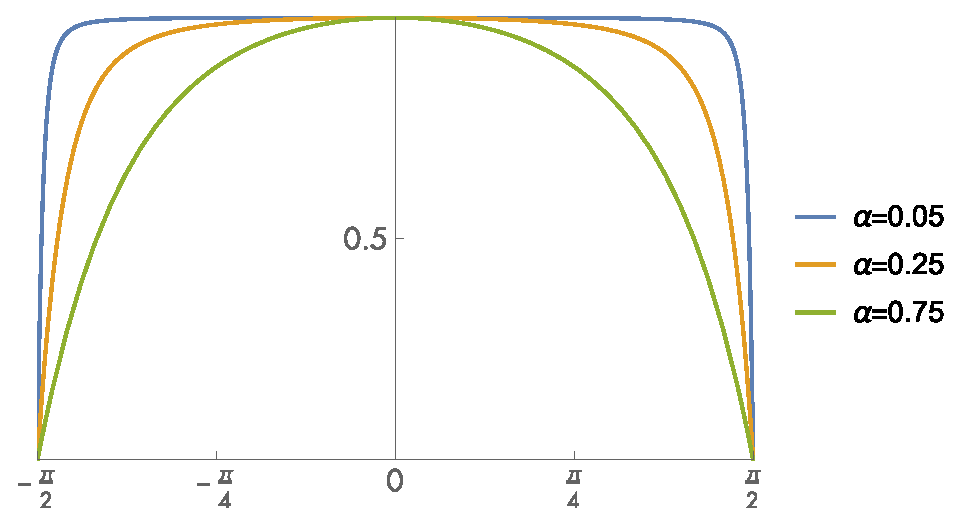
\includegraphics[width=0.75\linewidth]{Pictures/chap08/tr-g1-vs-alpha.eps}
    \caption{Trowbridge-Reitz分布的掩模遮挡函数$G_1({\bm\omega})$.
    增加曲面粗糙度(更高的$\alpha$值)让函数更快地降到零。}
    \label{fig:8.18}
\end{figure}

与微面分布的几何性质有关的最后一个很有用的函数是$G_1({\bm\omega}_{\mathrm{o}},{\bm\omega}_{\mathrm{i}})$,
它给出在微分区域中从方向${\bm\omega}_{\mathrm{o}}$和${\bm\omega}_{\mathrm{i}}$都可见的微面比例。
定义$G_1$需要一些额外假设\sidenote{译者注:原文中有时会简称$G$,为避免混淆,笔者改回为$G_1$,下同。}。
对于初学者,我们知道$G_1({\bm\omega}_{\mathrm{o}})$给出
从方向${\bm\omega}_{\mathrm{o}}$可见的微面比例,
而$G_1({\bm\omega}_{\mathrm{i}})$则给出从${\bm\omega}_{\mathrm{i}}$可见的比例就行。
如果我们假设微面从这两个方向均可见的概率就是独立地从每个方向可见的概率,则我们有
\begin{align*}
    G_1({\bm\omega}_{\mathrm{o}},{\bm\omega}_{\mathrm{i}})=G_1({\bm\omega}_{\mathrm{o}})G_1({\bm\omega}_{\mathrm{i}})\, .
\end{align*}
然而实践中,这些概率并不独立,该公式低估了$G_1$.
为了理解为什么这样,考虑${\bm\omega}_{\mathrm{o}}={\bm\omega}_{\mathrm{i}}$的情况;
该情况下任意从${\bm\omega}_{\mathrm{o}}$可见的微面也会从${\bm\omega}_{\mathrm{i}}$可见,
所以$G_1({\bm\omega}_{\mathrm{o}},{\bm\omega}_{\mathrm{i}})=G_1({\bm\omega}_{\mathrm{o}})=G_1({\bm\omega}_{\mathrm{i}})$.
因为$G_1({\bm\omega})\le 1$,所以该情况下它们的乘积会造成$G_1({\bm\omega}_{\mathrm{o}},{\bm\omega}_{\mathrm{i}})$太小
(除非$G_1({\bm\omega})=1$,但这通常只在${\bm\omega}=(0,0,1)$时成立)。
更普遍的是,两个方向越接近,$G_1({\bm\omega}_{\mathrm{o}})$和$G_1({\bm\omega}_{\mathrm{i}})$之间越相关。

假设微面上的给定点越高,微面就越可能可见,则可以推导出更精确的模型。该假设导出的模型是
\begin{align*}
    G_1({\bm\omega}_{\mathrm{o}},{\bm\omega}_{\mathrm{i}})=\frac{1}{1+\Lambda({\bm\omega}_{\mathrm{o}})+\Lambda({\bm\omega}_{\mathrm{i}})}\, .
\end{align*}
该近似在实践中相当准确,也是我们在pbrt中要用的。
详见本章末“扩展阅读”一节关于该函数的推导与更多定义
函数$G_1({\bm\omega}_{\mathrm{o}},{\bm\omega}_{\mathrm{i}})$的复杂方法的信息指南。
\begin{lstlisting}
`\refcode{MicrofacetDistribution Public Methods}{+=}\lastnext{MicrofacetDistributionPublicMethods}`
`\refvar{Float}{}` `\initvar[MicrofacetDistribution::G]{G}{}`(const `\refvar{Vector3f}{}` &wo, const `\refvar{Vector3f}{}` &wi) const {
    return 1 / (1 + `\refvar[MicrofacetDistribution::Lambda]{Lambda}{}`(wo) + `\refvar[MicrofacetDistribution::Lambda]{Lambda}{}`(wi));
}
\end{lstlisting}

\subsection{Torrance-Sparrow模型}\label{sub:Torrance-Sparrow模型}
\citet{Torrance:67}开发了一个早期微面模型来对金属曲面建模。
他们把曲面建模为完全光滑的镜像微面集合。
因为微面是完美镜面反射的,所以只有法线等于\keyindex{半角向量}{half-angle vector}{vector向量}
\sidenote{译者注:符号$\widehat{}$表示规范化为单位向量。}
\begin{align*}
    {\bm\omega}_{\mathrm{h}}=\widehat{{\bm\omega}_{\mathrm{i}}+{\bm\omega}_{\mathrm{o}}}
\end{align*}
的微面可以产生从${\bm\omega}_{\mathrm{i}}$到${\bm\omega}_{\mathrm{o}}$的
完美镜面反射(\reffig{8.19})。
\begin{figure}[htbp]
    \centering
    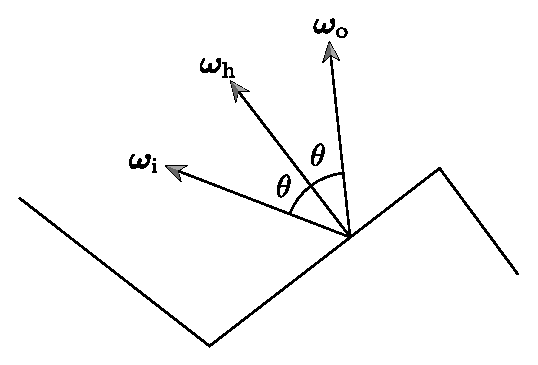
\includegraphics[width=0.5\linewidth]{Pictures/chap08/SpecularMicrofacetReflection.eps}
    \caption{对于完美镜面微面与给定的一对方向${\bm\omega}_{\mathrm{i}}$和${\bm\omega}_{\mathrm{o}}$,
    只有法线为${\bm\omega}_{\mathrm{h}}=\widehat{{\bm\omega}_{\mathrm{i}}+{\bm\omega}_{\mathrm{o}}}$的
    微面会把光线从${\bm\omega}_{\mathrm{i}}$反射到${\bm\omega}_{\mathrm{o}}$。}
    \label{fig:8.19}
\end{figure}

推导Torrance-Sparrow模型有许多有趣的步骤;我们将在这里详细介绍它。
首先,考虑微分通量$\mathrm{d}\varPhi_{\mathrm{h}}$入射到
朝向${\bm\omega}_{\mathrm{i}}$和${\bm\omega}_{\mathrm{o}}$的
半角${\bm\omega}_{\mathrm{h}}$方向的微面上。
根据辐射亮度的定义\refeq{5.2},它即
\sidenote{译者注:原文该式漏掉了${\bm\omega}_{\mathrm{i}}$的下标$\mathrm{i}$,此处已修正;
原文对通量的微分记作一阶,笔者改为了二阶。}
\begin{align*}
    \mathrm{d}^2\varPhi_{\mathrm{h}}=L_{\mathrm{i}}({\bm\omega}_{\mathrm{i}})
    \mathrm{d}{\bm\omega}_{\mathrm{i}}\mathrm{d}A^{\perp}({\bm\omega}_{\mathrm{h}})
    =L_{\mathrm{i}}({\bm\omega}_{\mathrm{i}})\mathrm{d}{\bm\omega}_{\mathrm{i}}
    \cos\theta_{\mathrm{h}}\mathrm{d}A({\bm\omega}_{\mathrm{h}})\, ,
\end{align*}
其中我们把朝向为${\bm\omega}_{\mathrm{h}}$的微面面积记作$\mathrm{d}A({\bm\omega}_{\mathrm{h}})$,
把${\bm\omega}_{\mathrm{i}}$和${\bm\omega}_{\mathrm{h}}$间夹角的余弦记作$\cos\theta_{\mathrm{h}}$(\reffig{8.20})。

\begin{figure}[htbp]
    \centering
    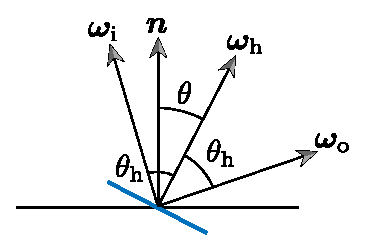
\includegraphics[width=0.35\linewidth]{Pictures/chap08/TorranceSparrowSetting.eps}
    \caption{推导Torrance-Sparrow模型的情形。
    对于方向${\bm\omega}_{\mathrm{i}}$和${\bm\omega}_{\mathrm{o}}$,
    只有法线为${\bm\omega}_{\mathrm{h}}$的微面会反射光线。
    ${\bm\omega}_{\mathrm{h}}$和$\bm n$之间的角度记作$\theta$,
    ${\bm\omega}_{\mathrm{h}}$和${\bm\omega}_{\mathrm{o}}$间的夹角记作$\theta_{\mathrm{h}}$
    (${\bm\omega}_{\mathrm{h}}$和${\bm\omega}_{\mathrm{i}}$间的夹角也必然是$\theta_{\mathrm{h}}$)。}
    \label{fig:8.20}
\end{figure}

朝向为${\bm\omega}_{\mathrm{h}}$的微面的微分面积为
\begin{align*}
    \mathrm{d}A({\bm\omega}_{\mathrm{h}})=D({\bm\omega}_{\mathrm{h}})\mathrm{d}{\bm\omega}_{\mathrm{h}}\mathrm{d}A\, .
\end{align*}
该乘积的前两项描述了每单位面积上具有正确朝向的微面的微分面积,
而$\mathrm{d}A$项将其转化为微分面积。因此
\sidenote{译者注:原文该式漏掉了${\bm\omega}_{\mathrm{i}}$的下标$\mathrm{i}$,此处已修正;
原文对通量的微分记作一阶,笔者改为了二阶。}
\begin{align}\label{eq:8.15}
    \mathrm{d}^2\varPhi_{\mathrm{h}}=L_{\mathrm{i}}({\bm\omega}_{\mathrm{i}})
    \mathrm{d}{\bm\omega}_{\mathrm{i}}\cos\theta_{\mathrm{h}}
    D({\bm\omega}_{\mathrm{h}})\mathrm{d}{\bm\omega}_{\mathrm{h}}\mathrm{d}A\, .
\end{align}
如果我们假设微面各自根据菲涅耳定律反射光线,则出射通量为
\begin{align}\label{eq:8.16}
    \mathrm{d}^2\varPhi_{\mathrm{o}}=F_{\mathrm{r}}({\bm\omega}_{\mathrm{o}})\mathrm{d}^2\varPhi_{\mathrm{h}}\, .
\end{align}
再次利用辐射亮度的定义,反射的出射亮度为
\begin{align*}
    L({\bm\omega}_{\mathrm{o}})=\frac{\mathrm{d}^2\varPhi_{\mathrm{o}}}
    {\cos\theta_{\mathrm{o}}\mathrm{d}{\bm\omega}_{\mathrm{o}}\mathrm{d}A}\, .
\end{align*}
如果我们把\refeq{8.16}代入上式,再把\refeq{8.15}代入其结果,则有
\begin{align*}
    L({\bm\omega}_{\mathrm{o}})=\frac{F_{\mathrm{r}}({\bm\omega}_{\mathrm{o}})
    L_{\mathrm{i}}({\bm\omega}_{\mathrm{i}})\mathrm{d}{\bm\omega}_{\mathrm{i}}\cos\theta_{\mathrm{h}}
    D({\bm\omega}_{\mathrm{h}})\mathrm{d}{\bm\omega}_{\mathrm{h}}\mathrm{d}A}
    {\cos\theta_{\mathrm{o}}\mathrm{d}{\bm\omega}_{\mathrm{o}}\mathrm{d}A}\, .
\end{align*}

在\refsub{微面BxDF}中,我们将在镜面反射条件下推导
出$\mathrm{d}{\bm\omega}_{\mathrm{h}}$与$\mathrm{d}{\bm\omega}_{\mathrm{o}}$的重要关系
\sidenote{译者注:尽管最后\refeq{8.18}是正确的,但笔者认为这里的推导可能包含了某些错误。
作者在\refsub{镜面反射}中专门强调了$f_\mathrm{r}({\bm p},{\bm \omega}_\mathrm{o},{\bm \omega}_\mathrm{i})$的形式
必须遵循该节第一个等式表达的约束,此时里面含有
项$\delta_{\mathrm{r}}({\bm\omega}_{\mathrm{i}}-{\bm\omega}_{\mathrm{r}})$,
该项在推导中必然导致需要处理$\mathrm{d}{\bm\omega}_{\mathrm{h}}$对$\mathrm{d}{\bm\omega}_{\mathrm{i}}$的变化关系,
而不是这里的$\mathrm{d}{\bm\omega}_{\mathrm{h}}$对$\mathrm{d}{\bm\omega}_{\mathrm{o}}$的关系。
此外这里的反射光比例用的记号也从之前的$F_{\mathrm{r}}({\bm\omega}_{\mathrm{i}})$改
为$F_{\mathrm{r}}({\bm\omega}_{\mathrm{o}})$,与前文不一致。
不过反射模型有很好的对称性,这种错误被抵消了。
同样的错误也出现在后文的BTDF推导中。详见\refeq{8.19}附近的旁注。
这种错误在这一段内容附近是系统性的,同时牵涉正文和代码,所以笔者不作修改,只做提示。}:
\begin{align}\label{eq:8.17}
    \mathrm{d}{\bm\omega}_{\mathrm{h}}=\frac{\mathrm{d}{\bm\omega}_{\mathrm{o}}}{4\cos\theta_{\mathrm{h}}}\, .
\end{align}
我们可以把该关系代入到之前的方程并化简,得到
\begin{align*}
    L({\bm\omega}_{\mathrm{o}})=\frac{F_{\mathrm{r}}({\bm\omega}_{\mathrm{o}})
    L_{\mathrm{i}}({\bm\omega}_{\mathrm{i}})D({\bm\omega}_{\mathrm{h}})\mathrm{d}{\bm\omega}_{\mathrm{i}}}
    {4\cos\theta_{\mathrm{o}}}\, .
\end{align*}
我们现在可以运用BRDF的定义\refeq{5.8}并添加几何衰减项$G({\bm\omega}_{\mathrm{o}},{\bm\omega}_{\mathrm{i}})$,
得到Torrance-Sparrow的BRDF:
\begin{align}\label{eq:8.18}
    f_{\mathrm{r}}({\bm\omega}_{\mathrm{o}},{\bm\omega}_{\mathrm{i}})=
    \frac{D({\bm\omega}_{\mathrm{h}})G({\bm\omega}_{\mathrm{o}},{\bm\omega}_{\mathrm{i}})
    F_{\mathrm{r}}({\bm\omega}_{\mathrm{o}})}{4\cos\theta_{\mathrm{o}}\cos\theta_{\mathrm{i}}}\, .
\end{align}

Torrance-Sparrow模型的一个优点是其推导不依赖于所用的特定微面分布。
此外,它也不依赖特定的菲涅耳函数,所以导体和介电质都可以它。
然而,推导中用的$\mathrm{d}{\bm\omega}_{\mathrm{h}}$与$\mathrm{d}{\bm\omega}_{\mathrm{o}}$的关系
要依赖微面的镜面反射假设。

\refvar{MicrofacetReflection}{}用Torrance-Sparrow模型实现通用的基于微面的BRDF。
\begin{lstlisting}
`\refcode{BxDF Declarations}{+=}\lastnext{BxDFDeclarations}`
class `\initvar{MicrofacetReflection}{}` : public `\refvar{BxDF}{}` {
public:
    `\refcode{MicrofacetReflection Public Methods}{}`
private:
    `\refcode{MicrofacetReflection Private Data}{}`
};
\end{lstlisting}
它的构造函数接收反射率,即指向一个\refvar{MicrofacetDistribution}{}实现的指针,以及一个菲涅耳函数。
\begin{lstlisting}
`\initcode{MicrofacetReflection Public Methods}{=}`
`\refvar{MicrofacetReflection}{}`(const `\refvar{Spectrum}{}` &R,
        `\refvar{MicrofacetDistribution}{}` *distribution, `\refvar{Fresnel}{}` *fresnel)
    : `\refvar{BxDF}{}`(`\refvar{BxDFType}{}`(`\refvar[BSDFREFLECTION]{BSDF\_REFLECTION}{}` | `\refvar{BSDFGLOSSY}{BSDF\_GLOSSY}`)), `\refvar[MicrofacetReflection::R]{R}{}`(R),
      `\refvar[MicrofacetReflection::distribution]{distribution}{}`(distribution), `\refvar[MicrofacetReflection::fresnel]{fresnel}{}`(fresnel) { }
\end{lstlisting}
\begin{lstlisting}
`\initcode{MicrofacetReflection Private Data}{=}`
const `\refvar{Spectrum}{}` `\initvar[MicrofacetReflection::R]{R}{}`;
const `\refvar{MicrofacetDistribution}{}` *`\initvar[MicrofacetReflection::distribution]{distribution}{}`;
const `\refvar{Fresnel}{}` *`\initvar[MicrofacetReflection::fresnel]{fresnel}{}`;
\end{lstlisting}

求Torrance-Sparrow的BRDF的各项值很简单。
对于菲涅耳项,回想在给定镜面反射下,${\bm\omega}_{\mathrm{h}}$与${\bm\omega}_{\mathrm{i}}$和${\bm\omega}_{\mathrm{o}}$之间的
角度均为$\theta_{\mathrm{h}}$,所以我们用哪个向量来计算$\theta_{\mathrm{h}}$的余弦都没关系。
我们就选${\bm\omega}_{\mathrm{i}}$.
\begin{lstlisting}
`\refcode{BxDF Method Definitions}{+=}\lastnext{BxDFMethodDefinitions}`
`\refvar{Spectrum}{}` `\refvar{MicrofacetReflection}{}`::`\initvar[MicrofacetReflection::f]{f}{}`(const `\refvar{Vector3f}{}` &wo,
        const `\refvar{Vector3f}{}` &wi) const {
    `\refvar{Float}{}` cosThetaO = `\refvar{AbsCosTheta}{}`(wo), cosThetaI = `\refvar{AbsCosTheta}{}`(wi);
    `\refvar{Vector3f}{}` wh = wi + wo;
    `\refcode{Handle degenerate cases for microfacet reflection}{}`
    wh = `\refvar{Normalize}{}`(wh);
    `\refvar{Spectrum}{}` F = `\refvar[MicrofacetReflection::fresnel]{fresnel}{}`->`\refvar[Fresnel::Evaluate]{Evaluate}{}`(`\refvar{Dot}{}`(wi, wh));
    return `\refvar[MicrofacetReflection::R]{R}{}` * `\refvar[MicrofacetReflection::distribution]{distribution}{}`->`\refvar[MicrofacetDistribution::D]{D}{}`(wh) * `\refvar[MicrofacetReflection::distribution]{distribution}{}`->`\refvar[MicrofacetDistribution::G]{G}{}`(wo, wi) * F /
           (4 * cosThetaI * cosThetaO);
}
\end{lstlisting}
还需要专门处理入射和出射方向处于掠角时的两种边界情况
以避免求BRDF值时生成NaN值。
\begin{lstlisting}
`\initcode{Handle degenerate cases for microfacet reflection}{=}`
if (cosThetaI == 0 || cosThetaO == 0) return `\refvar{Spectrum}{}`(0.);
if (wh.x == 0 && wh.y == 0 && wh.z == 0) return `\refvar{Spectrum}{}`(0.);
\end{lstlisting}

也可为表现为完美镜面透射的微面定义透射它时的BTDF。
该情形下,从折射率为$\eta_{\mathrm{i}}$的介质
透射到折射率为$\eta_{\mathrm{o}}$的介质
\sidenote{译者注:原文误写为$\eta_{\mathrm{t}}$,已修正。},
则$\mathrm{d}{\bm\omega}_{\mathrm{h}}$与$\mathrm{d}{\bm\omega}_{\mathrm{o}}$的关系为
\sidenote{译者注:前文透射时的出射方向${\bm\omega}_{\mathrm{t}}$在这里也用${\bm\omega}_{\mathrm{o}}$统一表示了。}:
\begin{align*}
    \mathrm{d}{\bm\omega}_{\mathrm{h}}=\frac{\eta^2_{\mathrm{o}}
    |{\bm\omega}_{\mathrm{o}}\cdot{\bm\omega}_{\mathrm{h}}|\mathrm{d}{\bm\omega}_{\mathrm{o}}}
    {(\eta_{\mathrm{i}}({\bm\omega}_{\mathrm{i}}\cdot{\bm\omega}_{\mathrm{h}})
    +\eta_{\mathrm{o}}({\bm\omega}_{\mathrm{o}}\cdot{\bm\omega}_{\mathrm{h}}))^2}\, .
\end{align*}

在推导Torrance-Sparrow的BRDF时可以用该关系替代\refeq{8.17}。结果为
\sidenote{译者注:和前面BRDF的情况类似,笔者认为\refeq{8.19}的推导存在错误,
应该是利用$\mathrm{d}{\bm\omega}_{\mathrm{h}}$对$\mathrm{d}{\bm\omega}_{\mathrm{i}}$的关系进行推导才对。
新书第4版9.7节中确实按这种方式改了,得到了与这里\refeq{8.19}不一样的结果,这可能意味着原作者也发现了这一错误。
笔者怀疑这些错误可能是原作者从\citet{10.5555/2383847.2383874}的论文继承来。
该论文的推导没有大问题,但唯独其中假设微面BSDF形式的第9式和本文\refsub{镜面反射}的说法冲突。
本文\refsub{镜面反射}已经说明了其中的$\delta$项关键变量应该包含${\bm\omega}_{\mathrm{i}}$,
但论文第9式却用的${\bm\omega}_{\mathrm{o}}$,意外对调了入射和出射关系。
原作者可能没有注意到这个细节,直接取用了论文最后的结果,引入了矛盾。
因为这些错误牵涉较多,笔者没有修正,仅作提示。
重新整理的推导可以参见笔者补充的\refsec{译者补充:微面模型相关推导}。}
\begin{align}\label{eq:8.19}
    f_{\mathrm{r}}({\bm\omega}_{\mathrm{o}},{\bm\omega}_{\mathrm{i}})=
    \frac{D({\bm\omega}_{\mathrm{h}})G({\bm\omega}_{\mathrm{o}},{\bm\omega}_{\mathrm{i}})
    (1-F_{\mathrm{r}}({\bm\omega}_{\mathrm{o}}))}{(({\bm\omega}_{\mathrm{o}}\cdot{\bm\omega}_{\mathrm{h}})
    +\eta({\bm\omega}_{\mathrm{i}}\cdot{\bm\omega}_{\mathrm{h}}))^2}
    \frac{|{\bm\omega}_{\mathrm{i}}\cdot{\bm\omega}_{\mathrm{h}}|
    |{\bm\omega}_{\mathrm{o}}\cdot{\bm\omega}_{\mathrm{h}}|}
    {\cos\theta_{\mathrm{o}}\cos\theta_{\mathrm{i}}}\, ,
\end{align}
其中$\displaystyle\eta=\frac{\eta_{\mathrm{i}}}{\eta_{\mathrm{o}}}$.
对于镜面透射,半角向量为
\begin{align*}
    {\bm\omega}_{\mathrm{h}}={\bm\omega}_{\mathrm{o}}+\eta{\bm\omega}_{\mathrm{i}}\, .
\end{align*}
(你可能想通过\refeq{8.8}验证该向量规范化后能让方向${\bm\omega}_{\mathrm{o}}$折射到${\bm\omega}_{\mathrm{i}}$.)

类\refvar{MicrofacetTransmission}{}实现该BTDF。
\begin{lstlisting}
`\refcode{BxDF Declarations}{+=}\lastnext{BxDFDeclarations}`
class `\initvar{MicrofacetTransmission}{}` : public `\refvar{BxDF}{}` {
public:
    `\refcode{MicrofacetTransmission Public Methods}{}`
private:
    `\refcode{MicrofacetTransmission Private Data}{}`
};
\end{lstlisting}
\begin{lstlisting}
`\initcode{MicrofacetTransmission Public Methods}{=}\initnext{MicrofacetTransmissionPublicMethods}`
`\refvar{MicrofacetTransmission}{}`(const `\refvar{Spectrum}{}` &T,
        `\refvar{MicrofacetDistribution}{}` *distribution, `\refvar{Float}{}` etaA, `\refvar{Float}{}` etaB,
        `\refvar{TransportMode}{}` mode)
    : `\refvar{BxDF}{}`(`\refvar{BxDFType}{}`(`\refvar[BSDFTRANSMISSION]{BSDF\_TRANSMISSION}{}` | `\refvar[BSDFGLOSSY]{BSDF\_GLOSSY}{}`)),
      `\refvar[MicrofacetTransmission::T]{T}{}`(T), `\refvar[MicrofacetTransmission::distribution]{distribution}{}`(distribution), `\refvar[MicrofacetTransmission::etaA]{etaA}{}`(etaA), `\refvar[MicrofacetTransmission::etaB]{etaB}{}`(etaB),
      `\refvar[MicrofacetTransmission::fresnel]{fresnel}{}`(etaA, etaB), `\refvar[MicrofacetTransmission::mode]{mode}{}`(mode) { }
\end{lstlisting}
\begin{lstlisting}
`\initcode{MicrofacetTransmission Private Data}{=}`
const `\refvar{Spectrum}{}` `\initvar[MicrofacetTransmission::T]{T}{}`;
const `\refvar{MicrofacetDistribution}{}` *`\initvar[MicrofacetTransmission::distribution]{distribution}{}`;
const `\refvar{Float}{}` `\initvar[MicrofacetTransmission::etaA]{etaA}{}`, `\initvar[MicrofacetTransmission::etaB]{etaB}{}`;
const `\refvar{FresnelDielectric}{}` `\initvar[MicrofacetTransmission::fresnel]{fresnel}{}`;
const `\refvar{TransportMode}{}` `\initvar[MicrofacetTransmission::mode]{mode}{}`;
\end{lstlisting}

它的方法\refvar[MicrofacetTransmission::f]{f}{()}直接誊写自\refeq{8.19}。
它的实现这里就不列出了\sidenote{译者注:笔者把它摘录回来了。}。
\begin{lstlisting}
`\refcode{MicrofacetTransmission Public Methods}{+=}\lastcode{MicrofacetTransmissionPublicMethods}`
`\refvar{Spectrum}{}` `\initvar[MicrofacetTransmission::f]{f}{}`(const `\refvar{Vector3f}{}` &wo, const `\refvar{Vector3f}{}` &wi) const {
    if (`\refvar{SameHemisphere}{}`(wo, wi)) return 0;  // transmission only

    `\refvar{Float}{}` cosThetaO = `\refvar{CosTheta}{}`(wo);
    `\refvar{Float}{}` cosThetaI = `\refvar{CosTheta}{}`(wi);
    if (cosThetaI == 0 || cosThetaO == 0) return `\refvar{Spectrum}{}`(0);

    // Compute ${\bm\omega}_{\mathrm{h}}$ from ${\bm\omega}_{\mathrm{o}}$ and ${\bm\omega}_{\mathrm{i}}$ for microfacet transmission
    `\refvar{Float}{}` eta = `\refvar{CosTheta}{}`(wo) > 0 ? (`\refvar[MicrofacetTransmission::etaB]{etaB}{}` / `\refvar[MicrofacetTransmission::etaA]{etaA}{}`) : (`\refvar[MicrofacetTransmission::etaA]{etaA}{}` / `\refvar[MicrofacetTransmission::etaB]{etaB}{}`);
    `\refvar{Vector3f}{}` wh = `\refvar{Normalize}{}`(wo + wi * eta);
    if (wh.z < 0) wh = -wh;

    // Same side?
    if (`\refvar{Dot}{}`(wo, wh) * `\refvar{Dot}{}`(wi, wh) > 0) return `\refvar{Spectrum}{}`(0);

    `\refvar{Spectrum}{}` F = `\refvar[MicrofacetTransmission::fresnel]{fresnel}{}`.`\refvar[Fresnel::Evaluate]{Evaluate}{}`(`\refvar{Dot}{}`(wo, wh));

    `\refvar{Float}{}` sqrtDenom = `\refvar{Dot}{}`(wo, wh) + eta * `\refvar{Dot}{}`(wi, wh);
    `\refvar{Float}{}` factor = (mode == `\refvar{TransportMode}{}`::`\refvar{Radiance}{}`) ? (1 / eta) : 1;

    return (`\refvar{Spectrum}{}`(1.f) - F) * `\refvar[MicrofacetTransmission::T]{T}{}` *
        std::abs(`\refvar[MicrofacetTransmission::distribution]{distribution}{}`->`\refvar[MicrofacetDistribution::D]{D}{}`(wh) * `\refvar[MicrofacetTransmission::distribution]{distribution}{}`->`\refvar[MicrofacetDistribution::G]{G}{}`(wo, wi) * eta * eta *
                    `\refvar{AbsDot}{}`(wi, wh) * `\refvar{AbsDot}{}`(wo, wh) * factor * factor /
                    (cosThetaI * cosThetaO * sqrtDenom * sqrtDenom));
}
\end{lstlisting}

\reffig{8.21}展示了用反射和透射Torrance-Sparrow模型渲染的龙。
\begin{figure}[htbp]
    \centering
    \subfloat[微面反射]{\includegraphics[width=0.75\linewidth]{chap08/dragon-mf-reflect.png}\label{fig:8.21.1}}\\
    \subfloat[微面折射]{\includegraphics[width=0.75\linewidth]{chap08/dragon-mf-transmit.png}\label{fig:8.21.2}}
    \caption{用(a)反射和(b)透射特化的Torrance-Sparrow微面模型渲染的龙模型(感谢Christian Schüller提供模型)。}
    \label{fig:8.21}
\end{figure}

\reffig{8.22}比较了被光源模拟的远处环境照亮的两个分别具有各向同性和各项异性微面模型的球体外观。
\begin{figure}[htbp]
    \centering
    \includegraphics[width=\linewidth]{chap08/spheres-aniso.png}
    \caption{用各向同性微面分布(左)和各向异性分布(右)渲染的球体。
    注意各向异性模型下不同的镜面高光形状。我们这里用球体代替龙是因为
    像这样的各向异性模型依赖于曲面上切向量全局一致的分布以便按合理方式确定各向异性朝向。}
    \label{fig:8.22}
\end{figure}


\section{菲涅耳入射效应}\label{sec:菲涅耳入射效应}
图形学中许多BRDF模型都没有考虑到菲涅耳反射会减少到达多层物体底层光量的事实。
考虑一张抛光的木桌或者涂了光泽油漆的墙面:如果你正对着看向它们的表面,
你主要看到的是木头或油漆颜料的颜色。随着你把你的视角移向掠角,
你会看到更少的底色,因为它被随菲涅耳效应而增加的光泽反射淹没了。

本节中,我们将实现由\citet{AshikhminPhong,Ashikhmin01012000}
\sidenote{译者注:原文文献年份标注可能有误,已修正。}
开发的BRDF模型,它刻画了覆盖有光泽镜面表面的漫反射表面。
在考虑了菲涅耳效应后,来自漫反射曲面的的反射效应会由剩余能量量值调制。
\reffig{8.23}展示了该想法:当入射方向接近法线时,大部分光会透射到
漫反射层,漫反射项占主要部分。而当入射方向接近掠角时,主要反射模式则是光泽反射。
\reffig{12.19}的汽车模型就给它的车漆用的本模型。
\begin{lstlisting}
`\refcode{BxDF Declarations}{+=}\lastnext{BxDFDeclarations}`
class `\initvar{FresnelBlend}{}` : public `\refvar{BxDF}{}` {
public:
    `\refcode{FresnelBlend Public Methods}{}`
private:
    `\refcode{FresnelBlend Private Data}{}`
};
\end{lstlisting}

\begin{figure}[htbp]
    \centering
    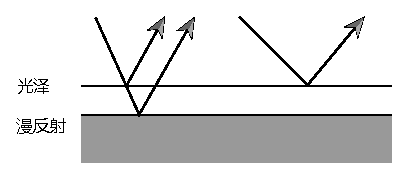
\includegraphics[width=0.65\linewidth]{Pictures/chap08/Fresnelincidence.eps}
    \caption{\refvar{FresnelBlend}{} BRDF刻画漫反射底层之上具有光泽层的曲面效果。
    随着向量${\bm\omega}_{\mathrm{i}}$和${\bm\omega}_{\mathrm{o}}$射入的角度移向掠角(右例),
    到达漫反射底层的光量因菲涅耳效应而减少,漫反射层变得更不明显了。}
    \label{fig:8.23}
\end{figure}

该模型接收两个光谱,一个表示漫反射和镜面反射,一个为光泽层的微面分布。
\begin{lstlisting}
`\refcode{BxDF Method Definitions}{+=}\lastnext{BxDFMethodDefinitions}`
`\refvar{FresnelBlend}{}`::`\refvar{FresnelBlend}{}`(const `\refvar{Spectrum}{}` &Rd, const `\refvar{Spectrum}{}` &Rs,
                           `\refvar{MicrofacetDistribution}{}` *distribution) 
    : `\refvar{BxDF}{}`(`\refvar{BxDFType}{}`(`\refvar[BSDFREFLECTION]{BSDF\_REFLECTION}{}` | `\refvar[BSDFGLOSSY]{BSDF\_GLOSSY}{}`)),
      `\refvar[FresnelBlend::Rd]{Rd}{}`(Rd), `\refvar[FresnelBlend::Rs]{Rs}{}`(Rs), `\refvar[FresnelBlend::distribution]{distribution}{}`(distribution) { }
\end{lstlisting}
\begin{lstlisting}
`\initcode{FresnelBlend Private Data}{=}`
const `\refvar{Spectrum}{}` `\initvar[FresnelBlend::Rd]{Rd}{}`, `\initvar[FresnelBlend::Rs]{Rs}{}`;
`\refvar{MicrofacetDistribution}{}` *`\initvar[FresnelBlend::distribution]{distribution}{}`;
\end{lstlisting}

该模型基于光泽镜面项和漫反射项的加权和。考虑到互易性和能量守恒,推导出光泽镜面项为
\sidenote{译者注:原文漏写了$F_{\mathrm{r}}$的下标,已修正。}
\begin{align*}
    f_{\mathrm{r}}({\bm p},{\bm\omega}_{\mathrm{o}},{\bm\omega}_{\mathrm{i}})
    =\frac{D({\bm\omega}_{\mathrm{h}})F_{\mathrm{r}}({\bm\omega}_{\mathrm{o}})}
    {4({\bm\omega}_{\mathrm{h}}\cdot{\bm\omega}_{\mathrm{i}})
    (\max(({\bm n}\cdot{\bm\omega}_{\mathrm{o}}),({\bm n}\cdot{\bm\omega}_{\mathrm{i}})))}\, ,
\end{align*}
其中$D({\bm\omega}_{\mathrm{h}})$是微面分布项,$F_{\mathrm{r}}({\bm\omega}_{\mathrm{o}})$表示
菲涅耳反射率。注意它和Torrance-Sparrow模型非常像。
\citeauthor{AshikhminPhong}的模型的关键是推导出仍然遵循互易性和
能量守恒的漫反射项。其推导依赖于\citet{Schlick1993}给出的对菲涅耳反射方程的近似,即
\begin{align*}
    F_{\mathrm{r}}(\cos\theta)=R+(1-R)(1-\cos\theta)^5\, ,
\end{align*}
其中$R$是按法线入射时的曲面反射率。

有了该菲涅耳项,下式的漫反射项就能以物理上较合理的方式成功刻画基于菲涅耳衰减的漫反射。
\begin{align*}
    f_{\mathrm{r}}({\bm p},{\bm\omega}_{\mathrm{o}},{\bm\omega}_{\mathrm{i}})
    =\frac{28R_{\mathrm{d}}}{23\pi}(1-R_{\mathrm{s}})
    \left(1-\left(1-\frac{1}{2}({\bm n}\cdot{\bm\omega}_{\mathrm{i}})\right)^5\right)
    \left(1-\left(1-\frac{1}{2}({\bm n}\cdot{\bm\omega}_{\mathrm{o}})\right)^5\right)\, .
\end{align*}

我们不会在这里引入对该结果的推导。
\begin{lstlisting}
`\initcode{FresnelBlend Public Methods}{=}`
`\refvar{Spectrum}{}` `\initvar{SchlickFresnel}{}`(`\refvar{Float}{}` cosTheta) const {
    auto pow5 = [](`\refvar{Float}{}` v) { return (v * v) * (v * v) * v; };
    return `\refvar[FresnelBlend::Rs]{Rs}{}` + pow5(1 - cosTheta) * (`\refvar{Spectrum}{}`(1.) - `\refvar[FresnelBlend::Rs]{Rs}{}`);
}
\end{lstlisting}
\begin{lstlisting}
`\refcode{BxDF Method Definitions}{+=}\lastnext{BxDFMethodDefinitions}`
`\refvar{Spectrum}{}` `\refvar{FresnelBlend}{}`::`\initvar[FresnelBlend::f]{f}{}`(const `\refvar{Vector3f}{}` &wo, const `\refvar{Vector3f}{}` &wi) const {
    auto pow5 = [](`\refvar{Float}{}` v) { return (v * v) * (v * v) * v; };
    `\refvar{Spectrum}{}` diffuse = (28.f/(23.f*`\refvar{Pi}{}`)) * `\refvar[FresnelBlend::Rd]{Rd}{}` *
        (`\refvar{Spectrum}{}`(1.f) - `\refvar[FresnelBlend::Rs]{Rs}{}`) * 
        (1 - pow5(1 - .5f * `\refvar{AbsCosTheta}{}`(wi))) *
        (1 - pow5(1 - .5f * `\refvar{AbsCosTheta}{}`(wo)));
    `\refvar{Vector3f}{}` wh = wi + wo;
    if (wh.x == 0 && wh.y == 0 && wh.z == 0) return `\refvar{Spectrum}{}`(0);
    wh = `\refvar{Normalize}{}`(wh);
    `\refvar{Spectrum}{}` specular = `\refvar[FresnelBlend::distribution]{distribution}{}`->`\refvar[MicrofacetDistribution::D]{D}{}`(wh) /
        (4 * `\refvar{AbsDot}{}`(wi, wh) *
         std::max(`\refvar{AbsCosTheta}{}`(wi), `\refvar{AbsCosTheta}{}`(wo))) *
         `\refvar{SchlickFresnel}{}`(`\refvar{Dot}{}`(wi, wh));
    return diffuse + specular;
}
\end{lstlisting}


\section{傅里叶基BSDF}\label{sec:傅里叶基BSDF}

{\noindent\hfil$=========$\hfil{\color{red}{施工分割线}}\hfil$=========$\

\section{扩展阅读}\label{sec:扩展阅读08}

\section{译者补充:微面模型相关推导}\label{sec:译者补充:微面模型相关推导}
\begin{remark}
    本节内容不是原书内容,而是译者根据\citet{heitz:hal-01024289}和\citet{10.5555/2383847.2383874}整理
    并推导后补充的,请酌情参考和斧正。
\end{remark}
\subsection{微面分布函数的定义与性质}\label{sub:微面分布函数的定义与性质}
如\reffig{08ex01-macrosurfaceMicrosurface},我们考虑一个足够小的宏曲面$\mathcal{G}$,设它是个绝对光滑的平面,具有法线$\bm n$.
微面模型中,真正粗糙起伏的曲面,即微曲面$\mathcal{M}$,是由许多偏离宏曲面的微面构成的。
或者说,微曲面$\mathcal{M}$上所有的点在方向$\bm n$上投影即得$\mathcal{G}$.
将宏曲面上的点记为${\bm p}_{\mathrm{g}}$,其周围的微分面元为$\mathrm{d}{\bm p}_{\mathrm{g}}$,
则宏曲面的面积为
\begin{align}
    S=\int\limits_{\mathcal{G}}\mathrm{d}{\bm p}_{\mathrm{g}}\, .
\end{align}

将$\mathcal{M}$上的点记作${\bm p}_{\mathrm{h}}$,该点处的法线记作${\bm\omega}_{\mathrm{h}}({\bm p}_{\mathrm{h}})$.
引入三维意义下的狄拉克$\delta$分布,
它满足$\displaystyle\int\limits_{\varOmega}\delta({\bm\omega})\mathrm{d}{\bm\omega}=1$.
并记$\delta_{\bm\omega}({\bm\omega}')=\delta({\bm\omega}'-{\bm\omega})$.
由此定义\keyindex{微面分布函数}{microfacet distribution function}{distribution分布}为
\sidenote{原论文全文假定$S=1$来讨论,不用除以面积,这里笔者的处理有所不同。}
\begin{align}\label{eq:08ex01-MicrosurfaceDistribution}
    D({\bm\omega})=\displaystyle\frac{1}{S}\int\limits_{\mathcal{M}}
    \delta_{\bm\omega}({\bm\omega}_{\mathrm{h}}({\bm p}_{\mathrm{h}}))
    \mathrm{d}{\bm p}_{\mathrm{h}}\, ,
\end{align}
其中狄拉克$\delta$分布和$D({\bm\omega}_{\mathrm{h}})$的量纲均为
球面度的倒数即$\displaystyle\frac{1}{\text{sr}}$,也相当于无量纲。

\begin{figure}[htbp]
    \centering
    \includegraphics[width=0.6\linewidth]{Pictures/chap08/macrosurfaceMicrosurface.eps}
    \caption{宏曲面(黑色)与微曲面(红色)。}
    \label{fig:08ex01-macrosurfaceMicrosurface}
\end{figure}

我们可以把${\bm\omega}_{\mathrm{h}}$视作从$\mathcal{M}$到整个方向空间$\varOmega$的映射。
注意$\varOmega$包含了球心到完整球面上任意一点的所有可能方向(总立体角为$4\pi$,尽管该映射不一定能覆盖全)。
现在考虑$\mathcal{M}$和$\varOmega$各自的子集$\mathcal{M'}$和$\varOmega'$,
并设它们满足以下条件:点${\bm p}_{\mathrm{h}}$属于$\mathcal{M'}$当且仅当
该点处的微面法线${\bm\omega}_{\mathrm{h}}({\bm p}_{\mathrm{h}})$属于$\varOmega'$,即
\begin{align}
    {\bm p}_{\mathrm{h}}\in\mathcal{M'}\Leftrightarrow
    {\bm\omega}_{\mathrm{h}}({\bm p}_{\mathrm{h}})\in\varOmega'\, .
\end{align}
由此利用积分换元可得微面分布函数具有计算指定微曲面面积的能力:
\begin{align}
    \label{eq:08ex01-microsurfaceArea}
    \int\limits_{\mathcal{M}'}\mathrm{d}{\bm p}_{\mathrm{h}}
    =S\int\limits_{\varOmega'}D({\bm\omega}_{\mathrm{h}})\mathrm{d}{\bm\omega}_{\mathrm{h}}\, .
\end{align}
而整个微曲面面积就是
\begin{align}
    \int\limits_{\mathcal{M}}\mathrm{d}{\bm p}_{\mathrm{h}}
    =S\int\limits_{\varOmega}D({\bm\omega}_{\mathrm{h}})\mathrm{d}{\bm\omega}_{\mathrm{h}}\, .
\end{align}

进一步地,对于任意关于微面法线的函数$f({\bm\omega}_{\mathrm{h}})$,
利用$D({\bm\omega}_{\mathrm{h}})$可将空间积分与统计积分相互转化:
\begin{align}
    \int\limits_{\mathcal{M}}f({\bm\omega}_{\mathrm{h}}({\bm p}_{\mathrm{h}}))\mathrm{d}{\bm p}_{\mathrm{h}}
    =S\int\limits_{\varOmega}f({\bm\omega}_{\mathrm{h}})
    D({\bm\omega}_{\mathrm{h}})\mathrm{d}{\bm\omega}_{\mathrm{h}}\, .
\end{align}

反之,对于任意定义在$\mathcal{M}$上的函数$g({\bm p}_{\mathrm{h}})$,
我们可以定义对应的统计函数$g({\bm\omega}_{\mathrm{h}})$为
\sidenote{这里原论文为了在记号上强调二者的联系,仍然使用了符号$g$,
    但读者应明白这是一个新的函数了。后面\refeq{08ex01-StaticMaskFunc}等的情况类似。}:
\begin{align}\label{eq:08ex01-StaticFunc}
    g({\bm\omega})=\frac{\displaystyle\int\limits_{\mathcal{M}}
    \delta_{\bm\omega}({\bm\omega}_{\mathrm{h}}({\bm p}_{\mathrm{h}}))
    g({\bm p}_{\mathrm{h}})\mathrm{d}{\bm p}_{\mathrm{h}}}
    {\displaystyle\int\limits_{\mathcal{M}}
    \delta_{\bm\omega}({\bm\omega}_{\mathrm{h}}({\bm p}_{\mathrm{h}}))
    \mathrm{d}{\bm p}_{\mathrm{h}}}\, .
\end{align}
该函数也可以实现空间积分与统计积分的相互转化:
\begin{align}\label{eq:08ex01-TransferSpaceStatic}
    \int\limits_{\mathcal{M}}g({\bm p}_{\mathrm{h}})\mathrm{d}{\bm p}_{\mathrm{h}}
    =S\int\limits_{\varOmega}g({\bm\omega}_{\mathrm{h}})
    D({\bm\omega}_{\mathrm{h}})\mathrm{d}{\bm\omega}_{\mathrm{h}}\, .
\end{align}

如\reffig{08ex01-ProjectionsMicrofacetArea},理解以上推导后,我们可以计算以下面积。
\begin{figure}[htbp]
    \centering
    \includegraphics[width=0.5\linewidth]{Pictures/chap08/ProjectionsMicrofacet.eps}
    \caption{微面可见部分在${\bm\omega}_{\mathrm{o}}$上的投影面积。}
    \label{fig:08ex01-ProjectionsMicrofacetArea}
\end{figure}

首先,微曲面在宏曲面法线方向${\bm\omega}_{\mathrm{g}}$上的
投影面积(不论是否遮挡,且背向时记负值)为
\begin{align}
    \int\limits_{\mathcal{M}}({\bm\omega}_{\mathrm{h}}({\bm p}_{\mathrm{h}})
    \cdot{\bm\omega}_{\mathrm{g}})\mathrm{d}{\bm p}_{\mathrm{h}}
    =S\int\limits_{\varOmega}({\bm\omega}_{\mathrm{h}}\cdot{\bm\omega}_{\mathrm{g}})
    D({\bm\omega}_{\mathrm{h}})\mathrm{d}{\bm\omega}_{\mathrm{h}}
    =\int\limits_{\mathcal{G}}\mathrm{d}{\bm p}_{\mathrm{g}}=S\, .
\end{align}
注意上式同时给出了一个$D({\bm\omega}_{\mathrm{h}})$应满足的重要约束:
\begin{align}\label{eq:08ex01-McrofacetDistributionNormalization}
    \int\limits_{\varOmega}({\bm\omega}_{\mathrm{h}}\cdot{\bm\omega}_{\mathrm{g}})
    D({\bm\omega}_{\mathrm{h}})\mathrm{d}{\bm\omega}_{\mathrm{h}}=1\, .
\end{align}

接着我们从出射方向${\bm\omega}_{\mathrm{o}}$来观察曲面。此时宏曲面在${\bm\omega}_{\mathrm{o}}$上的投影面积为
\begin{align}
    \label{eq:08ex01-AreaMacrosurface}
    ({\bm\omega}_{\mathrm{o}}\cdot{\bm\omega}_{\mathrm{g}})S=S\cos\theta_{\mathrm{o}}\, ,
\end{align}
其中$\theta_{\mathrm{o}}$为${\bm\omega}_{\mathrm{o}}$与${\bm\omega}_{\mathrm{g}}$的夹角。

最后我们算得微面可见部分在${\bm\omega}_{\mathrm{o}}$上的投影面积为
\begin{align}\label{eq:08ex01-AreaProjectionsMicrofacetVisible}
    \int\limits_{\mathcal{M}}G_1({\bm p}_{\mathrm{h}},{\bm\omega}_{\mathrm{o}})
    \max({\bm\omega}_{\mathrm{h}}({\bm p}_{\mathrm{h}})\cdot{\bm\omega}_{\mathrm{o}},0)
    \mathrm{d}{\bm p}_{\mathrm{h}}\, ,
\end{align}
其中\keyindex{空间掩模函数}{spatial masking function}{masking function掩模函数}
$G_1({\bm p}_{\mathrm{h}},{\bm\omega}_{\mathrm{o}})$在${\bm p}_{\mathrm{h}}$被
遮挡时取0,否则取1. 而$\max$项则过滤了背向不可见的微面。
其对应的\keyindex{统计掩模函数}{statistical masking function}{masking function掩模函数}
$G_1({\bm\omega}_{\mathrm{h}},{\bm\omega}_{\mathrm{o}})$的值域为$[0,1]$,
它给出了从方向${\bm\omega}_{\mathrm{o}}$观察时,法线为${\bm\omega}_{\mathrm{h}}$的微面中可见的比例:
\begin{align}\label{eq:08ex01-StaticMaskFunc}
    G_1({\bm\omega},{\bm\omega}_{\mathrm{o}})
    =\frac{\displaystyle\int\limits_{\mathcal{M}}
    \delta_{\bm\omega}({\bm\omega}_{\mathrm{h}}({\bm p}_{\mathrm{h}}))
    G_1({\bm p}_{\mathrm{h}},{\bm\omega}_{\mathrm{o}})\mathrm{d}{\bm p}_{\mathrm{h}}}
    {\displaystyle\int\limits_{\mathcal{M}}
    \delta_{\bm\omega}({\bm\omega}_{\mathrm{h}}({\bm p}_{\mathrm{h}}))
    \mathrm{d}{\bm p}_{\mathrm{h}}}\, .
\end{align}
由此得到投影面积的另一计算方式:
\begin{align}
    \label{eq:08ex01-AreaMicrosurface}
    S\int\limits_{\varOmega}G_1({\bm\omega}_{\mathrm{h}},{\bm\omega}_{\mathrm{o}})
    \max({\bm\omega}_{\mathrm{h}}\cdot{\bm\omega}_{\mathrm{o}},0)
    D({\bm\omega}_{\mathrm{h}})\mathrm{d}{\bm\omega}_{\mathrm{h}}\, .
\end{align}

由于可见微面投影面积等于宏曲面投影面积,所以
结合\refeq{08ex01-AreaMacrosurface}和\refeq{08ex01-AreaMicrosurface}可得
基于物理的掩模函数$G_1$总是满足如下约束:
\begin{align}\label{eq:08ex01-CosThetaO}
    \cos\theta_{\mathrm{o}}=\int\limits_{\varOmega}
    G_1({\bm\omega}_{\mathrm{h}},{\bm\omega}_{\mathrm{o}})
    \max({\bm\omega}_{\mathrm{h}}\cdot{\bm\omega}_{\mathrm{o}},0)
    D({\bm\omega}_{\mathrm{h}})\mathrm{d}{\bm\omega}_{\mathrm{h}}\, .
\end{align}
注意这并不意味着该约束唯一确定了$G_1$,它常常有无数个解。
还需引入其他约束或假设才能限定为唯一解。
\reffig{08ex01-SameDistributionOfNormalsDifferentBRDFs}给出了这种不唯一性的例子。
\begin{figure}[htbp]
    \centering
    \includegraphics[width=0.75\linewidth]{Pictures/chap08/SameDistributionOfNormalsDifferentBRDFs.eps}
    \caption{具有相同微面分布函数$D({\bm\omega}_{\mathrm{h}})$但BRDF却不同的两种微面。}
    \label{fig:08ex01-SameDistributionOfNormalsDifferentBRDFs}
\end{figure}

此外,译者再补充两个\refeq{08ex01-StaticMaskFunc}可能让人感到困惑的地方:

第一个是记号的问题。$G_1({\bm\omega}_{\mathrm{h}},{\bm\omega}_{\mathrm{o}})$中
第一个自变量是${\bm\omega}_{\mathrm{h}}$,该变量应出现在其定义式中狄拉克$\delta$分布的下标,
但狄拉克$\delta$分布后面的括号内还有一个记号相同的函数${\bm\omega}_{\mathrm{h}}({\bm p}_{\mathrm{h}})$,
所以为了区分它们,\refeq{08ex01-StaticMaskFunc}中临时把第一个自变量改写为${\bm\omega}$.
笔者保留了原论文的这个做法,请读者注意区分。\refeq{08ex01-MicrosurfaceDistribution}、
\refeq{08ex01-StaticFunc}、\refeq{08ex01-AnotherStaticFunc}、\refeq{08-ex01-masking-g1-int}和
\refeq{08ex01-VCavityScatteringNormalDistribution}等也用了类似的临时记号。

第二个是定义的问题。细心的读者可能注意到,
比对\refeq{08ex01-AreaProjectionsMicrofacetVisible}和\refeq{08ex01-TransferSpaceStatic},
我们本该设
\begin{align}\label{eq:08ex01-AnotherSpaceFunc}
    g({\bm p}_{\mathrm{h}})=G_1({\bm p}_{\mathrm{h}},{\bm\omega}_{\mathrm{o}})
    \max({\bm\omega}_{\mathrm{h}}({\bm p}_{\mathrm{h}})\cdot{\bm\omega}_{\mathrm{o}},0)\, ,
\end{align}
此时使得\refeq{08ex01-TransferSpaceStatic}成立的$g({\bm\omega}_{\mathrm{h}})$应该是
把\refeq{08ex01-AnotherSpaceFunc}带入\refeq{08ex01-StaticFunc}得到的
\begin{align}\label{eq:08ex01-AnotherStaticFunc}
    g({\bm\omega})=\frac{\displaystyle\int\limits_{\mathcal{M}}
    \delta_{\bm\omega}({\bm\omega}_{\mathrm{h}}({\bm p}_{\mathrm{h}}))
    G_1({\bm p}_{\mathrm{h}},{\bm\omega}_{\mathrm{o}})
    \max({\bm\omega}_{\mathrm{h}}({\bm p}_{\mathrm{h}})\cdot{\bm\omega}_{\mathrm{o}},0)
    \mathrm{d}{\bm p}_{\mathrm{h}}}
    {\displaystyle\int\limits_{\mathcal{M}}
    \delta_{\bm\omega}({\bm\omega}_{\mathrm{h}}({\bm p}_{\mathrm{h}}))
    \mathrm{d}{\bm p}_{\mathrm{h}}}\, .
\end{align}
将上式回代\refeq{08ex01-TransferSpaceStatic}的右边后,
读者会发现它和\refeq{08ex01-AreaMicrosurface}并不是完全一样的——
后者相当于把前者内层积分中的项$\max({\bm\omega}_{\mathrm{h}}({\bm p}_{\mathrm{h}})\cdot{\bm\omega}_{\mathrm{o}},0)$
(里面的${\bm\omega}_{\mathrm{h}}$是函数)提到外层积分中
变成了$\max({\bm\omega}_{\mathrm{h}}\cdot{\bm\omega}_{\mathrm{o}},0)$
(里面的${\bm\omega}_{\mathrm{h}}$是变量)。
一般来说积分变量并不能随便外提,但因为这里内层积分中含有狄拉克$\delta$分布,
它使得此处外提$\max$项的做法恰好没有改变整个式子的值。
所以原论文中作出简化处理,相当于令$g({\bm p}_{\mathrm{h}})=G_1({\bm p}_{\mathrm{h}},{\bm\omega}_{\mathrm{o}})$,
此时对应的$g({\bm\omega}_{\mathrm{h}})$即为\refeq{08ex01-StaticMaskFunc}中
的$G_1({\bm\omega}_{\mathrm{h}},{\bm\omega}_{\mathrm{o}})$.
不过原作者并未交代这样的细节。后面\refeq{08ex01-RadianceMicrofacet}也用了类似技巧。

\subsection{基于微面模型的BRDF}\label{sub:基于微面模型的BRDF}
本节继承上节的记号。在微面尺度上,我们设微面上一点朝出射方向${\bm\omega}_{\mathrm{o}}$的辐亮度
为$L_{\mathcal{M}}({\bm\omega}_{\mathrm{h}}({\bm p}_{\mathrm{h}}),{\bm\omega}_{\mathrm{o}})$.
则从宏观尺度看,该微面整体朝${\bm\omega}_{\mathrm{o}}$等价的出射
辐亮度$L_{\mathrm{o}}({\bm\omega}_{\mathrm{o}})$即为
微面尺度的辐亮度按出射方向可见投影面积比例的加权:
\begin{align}\label{eq:08ex01-RadianceMicrofacetAverageSum}
    L_{\mathrm{o}}({\bm\omega}_{\mathrm{o}})
    =\frac{\displaystyle\int\limits_{\mathcal{M}}
    {L_{\mathcal{M}}({\bm\omega}_{\mathrm{h}}({\bm p}_{\mathrm{h}}),{\bm\omega}_{\mathrm{o}})
    G_1({\bm p}_{\mathrm{h}},{\bm\omega}_{\mathrm{o}})
    \max({\bm\omega}_{\mathrm{h}}({\bm p}_{\mathrm{h}})\cdot{\bm\omega}_{\mathrm{o}},0)
    \mathrm{d}{\bm p}_{\mathrm{h}}}}
    {\displaystyle\int\limits_{\mathcal{M}}
    {G_1({\bm p}_{\mathrm{h}},{\bm\omega}_{\mathrm{o}})
    \max({\bm\omega}_{\mathrm{h}}({\bm p}_{\mathrm{h}})\cdot{\bm\omega}_{\mathrm{o}},0)
    \mathrm{d}{\bm p}_{\mathrm{h}}}}\, .
\end{align}
上式利用空间掩模函数\refeq{08ex01-StaticMaskFunc}转化为统计积分形式,
并将\refeq{08ex01-AreaProjectionsMicrofacetVisible}带入分母可得:
\begin{align}\label{eq:08ex01-RadianceMicrofacet}
    L_{\mathrm{o}}({\bm\omega}_{\mathrm{o}})
    =\frac{1}{\cos\theta_{\mathrm{o}}}\int\limits_{\varOmega}
    L_{\mathcal{M}}({\bm\omega}_{\mathrm{h}},{\bm\omega}_{\mathrm{o}})
    G_1({\bm\omega}_{\mathrm{h}},{\bm\omega}_{\mathrm{o}})
    \max({\bm\omega}_{\mathrm{h}}\cdot{\bm\omega}_{\mathrm{o}},0)
    D({\bm\omega}_{\mathrm{h}})\mathrm{d}{\bm\omega}_{\mathrm{h}}\, .
\end{align}
观察上式,我们把被积分项中对$L_{\mathcal{M}}({\bm\omega}_{\mathrm{h}},{\bm\omega}_{\mathrm{o}})$加权的系数
定义为\keyindex{可见法线分布}{distribution of visible normals}{distribution分布}:
\begin{align}\label{eq:08ex01-DistributionOfVisibleNormals}
    D_{{\bm\omega}_{\mathrm{o}}}({\bm\omega}_{\mathrm{h}})
    =\frac{G_1({\bm\omega}_{\mathrm{h}},{\bm\omega}_{\mathrm{o}})
        \max({\bm\omega}_{\mathrm{h}}\cdot{\bm\omega}_{\mathrm{o}},0)
        D({\bm\omega}_{\mathrm{h}})}{\cos\theta_{\mathrm{o}}}\, .
\end{align}
其中$\cos\theta_{\mathrm{o}}$如\refeq{08ex01-AreaMacrosurface}所述
即${\bm\omega}_{\mathrm{o}}\cdot{\bm\omega}_{\mathrm{g}}$,
于是\refeq{08ex01-RadianceMicrofacet}可以表示为:
\begin{align}\label{eq:08ex01-RadianceMacroOut}
    L_{\mathrm{o}}({\bm\omega}_{\mathrm{o}})
    =\int\limits_{\varOmega}L_{\mathcal{M}}({\bm\omega}_{\mathrm{h}},{\bm\omega}_{\mathrm{o}})
    D_{{\bm\omega}_{\mathrm{o}}}({\bm\omega}_{\mathrm{h}})\mathrm{d}{\bm\omega}_{\mathrm{h}}\, .
\end{align}
同时应注意到该定义下$D_{{\bm\omega}_{\mathrm{o}}}({\bm\omega}_{\mathrm{h}})$满足规范化性质:
\begin{align}\label{eq:08ex01-VisibleDistributionNormalization}
    \int\limits_{\varOmega}D_{{\bm\omega}_{\mathrm{o}}}({\bm\omega}_{\mathrm{h}})
    \mathrm{d}{\bm\omega}_{\mathrm{h}}=1\, .
\end{align}
若再结合\refeq{08ex01-CosThetaO},则$L_{\mathrm{o}}({\bm\omega}_{\mathrm{o}})$还可以表示为以下形式:
\begin{align}\label{eq:08ex01-RadianceMacroOutV2}
    L_{\mathrm{o}}({\bm\omega}_{\mathrm{o}})
    =\frac{\displaystyle\int\limits_{\varOmega}L_{\mathcal{M}}({\bm\omega}_{\mathrm{h}},{\bm\omega}_{\mathrm{o}})
    G_1({\bm\omega}_{\mathrm{h}},{\bm\omega}_{\mathrm{o}})
    \max({\bm\omega}_{\mathrm{h}}\cdot{\bm\omega}_{\mathrm{o}},0)
    D({\bm\omega}_{\mathrm{h}})\mathrm{d}{\bm\omega}_{\mathrm{h}}}
    {\displaystyle\int\limits_{\varOmega}G_1({\bm\omega}_{\mathrm{h}},{\bm\omega}_{\mathrm{o}})
    \max({\bm\omega}_{\mathrm{h}}\cdot{\bm\omega}_{\mathrm{o}},0)
    D({\bm\omega}_{\mathrm{h}})\mathrm{d}{\bm\omega}_{\mathrm{h}}}\, .
\end{align}

接下来我们利用微面尺度上的BRDF推导微面模型在宏观尺度下的BRDF。
把微面尺度上的BRDF记作$f_{\mathcal{M}}({\bm\omega}_{\mathrm{h}},{\bm\omega}_{\mathrm{o}},{\bm\omega}_{\mathrm{i}})$,
考虑到有效的角度范围,则根据\refeq{5.8}中BRDF的定义有
\begin{align}\label{eq:08ex01-MicrosurfaceBRDF}
    f_{\mathcal{M}}({\bm\omega}_{\mathrm{h}},{\bm\omega}_{\mathrm{o}},{\bm\omega}_{\mathrm{i}})
    =\frac{\mathrm{d} L_{\mathcal{M}}({\bm\omega}_{\mathrm{h}},{\bm\omega}_{\mathrm{o}})}
    {\max({\bm\omega}_{\mathrm{h}}\cdot{\bm\omega}_{\mathrm{i}},0)
    L_{\mathrm{i}}({\bm\omega}_{\mathrm{i}})\mathrm{d}{\bm\omega}_{\mathrm{i}}}\, ,
\end{align}
其中$L_{\mathrm{i}}({\bm\omega}_{\mathrm{i}})$是来自入射方向${\bm\omega}_{\mathrm{i}}$的辐亮度。
由此我们根据定义并结合\refeq{08ex01-RadianceMacroOut}、\refeq{08ex01-MicrosurfaceBRDF}、
\refeq{08ex01-DistributionOfVisibleNormals}得到宏观尺度下的BRDF为:
\begin{align}\label{eq:08ex01-MacroBRDFG1}
    f_{\mathrm{r}}({\bm\omega}_{\mathrm{o}},{\bm\omega}_{\mathrm{i}})
     & = \frac{\mathrm{d} L_{\mathrm{o}}({\bm\omega}_{\mathrm{o}})}
    {|{\bm\omega}_{\mathrm{g}}\cdot{\bm\omega}_{\mathrm{i}}|
    L_{\mathrm{i}}({\bm\omega}_{\mathrm{i}})\mathrm{d}{\bm\omega}_{\mathrm{i}}}
    = \frac{1}{|{\bm\omega}_{\mathrm{g}}\cdot{\bm\omega}_{\mathrm{i}}|}
    \int\limits_{\varOmega}\frac{\mathrm{d}L_{\mathcal{M}}({\bm\omega}_{\mathrm{h}},{\bm\omega}_{\mathrm{o}})}
    {L_{\mathrm{i}}({\bm\omega}_{\mathrm{i}})\mathrm{d}{\bm\omega}_{\mathrm{i}}}
    D_{{\bm\omega}_{\mathrm{o}}}({\bm\omega}_{\mathrm{h}})\mathrm{d}{\bm\omega}_{\mathrm{h}}\nonumber \\
     & = \frac{1}{|{\bm\omega}_{\mathrm{g}}\cdot{\bm\omega}_{\mathrm{i}}|}
    \int\limits_{\varOmega}f_{\mathcal{M}}({\bm\omega}_{\mathrm{h}},{\bm\omega}_{\mathrm{o}},{\bm\omega}_{\mathrm{i}})
    \max({\bm\omega}_{\mathrm{h}}\cdot{\bm\omega}_{\mathrm{i}},0)
    D_{{\bm\omega}_{\mathrm{o}}}({\bm\omega}_{\mathrm{h}})\mathrm{d}{\bm\omega}_{\mathrm{h}}\nonumber \\
     & = \frac{1}{|{\bm\omega}_{\mathrm{g}}\cdot{\bm\omega}_{\mathrm{i}}|
    |{\bm\omega}_{\mathrm{g}}\cdot{\bm\omega}_{\mathrm{o}}|}
    \int\limits_{\varOmega}f_{\mathcal{M}}({\bm\omega}_{\mathrm{h}},{\bm\omega}_{\mathrm{o}},{\bm\omega}_{\mathrm{i}})
    \max({\bm\omega}_{\mathrm{h}}\cdot{\bm\omega}_{\mathrm{i}},0)\nonumber                            \\
     & \qquad\qquad\max({\bm\omega}_{\mathrm{h}}\cdot{\bm\omega}_{\mathrm{o}},0)
    G_1({\bm\omega}_{\mathrm{h}},{\bm\omega}_{\mathrm{o}})
    D({\bm\omega}_{\mathrm{h}})\mathrm{d}{\bm\omega}_{\mathrm{h}}\, .
\end{align}

我们应注意到,上式考虑的其实是入射光在曲面上经历第一次反射后刚刚离开的情形,
并未考虑到反射的光线可能还会再命中曲面一次甚至多次然后从其他方向射出的情况。
然而我们在宏观尺度下的BRDF是定义在单次反射的情形下的,所以应排除掉这些光线。
为此,我们引入\keyindex{遮挡函数}{shadowing function}{}来到达这一效果。
实际中,我们通常直接使用联合的\keyindex{掩模遮挡函数}{masking-shadowing function}{}$G_2$来代替$G_1$,
它计入的微面比例要求在${\bm\omega}_{\mathrm{o}}$和${\bm\omega}_{\mathrm{i}}$上双向可见,此时
\begin{align}\label{eq:08ex01-MacroBRDFG2}
    f_{\mathrm{r}}({\bm\omega}_{\mathrm{o}},{\bm\omega}_{\mathrm{i}})
     & =\frac{1}{|{\bm\omega}_{\mathrm{g}}\cdot{\bm\omega}_{\mathrm{i}}||{\bm\omega}_{\mathrm{g}}\cdot{\bm\omega}_{\mathrm{o}}|}
    \int\limits_{\varOmega}f_{\mathcal{M}}({\bm\omega}_{\mathrm{h}},{\bm\omega}_{\mathrm{o}},{\bm\omega}_{\mathrm{i}})
    \max({\bm\omega}_{\mathrm{h}}\cdot{\bm\omega}_{\mathrm{i}},0)\nonumber                                                       \\
     & \qquad\qquad\max({\bm\omega}_{\mathrm{h}}\cdot{\bm\omega}_{\mathrm{o}},0)
    G_2({\bm\omega}_{\mathrm{h}},{\bm\omega}_{\mathrm{o}},{\bm\omega}_{\mathrm{i}})
    D({\bm\omega}_{\mathrm{h}})\mathrm{d}{\bm\omega}_{\mathrm{h}}\, .
\end{align}

最后,笔者认为对于透射的情况,将\refeq{08ex01-RadianceMicrofacetAverageSum}、
\refeq{08ex01-RadianceMicrofacet}、
\refeq{08ex01-DistributionOfVisibleNormals}、
\refeq{08ex01-RadianceMacroOutV2}、\refeq{08ex01-MicrosurfaceBRDF}、
\refeq{08ex01-MacroBRDFG1}、\refeq{08ex01-MacroBRDFG2}
中的$\max(\cdot,0)$项均改为对应的绝对值$|\cdot|$即可。

\subsection{镜面微面模型的BRDF}\label{sub:镜面微面模型的BRDF}
本节继承上节的记号。为了算出微面模型在宏观尺度下的BRDF,
即\refeq{08ex01-MacroBRDFG1}或\refeq{08ex01-MacroBRDFG2},
我们需要知道微面尺度下的BRDF即$f_{\mathcal{M}}({\bm\omega}_{\mathrm{h}},{\bm\omega}_{\mathrm{o}},{\bm\omega}_{\mathrm{i}})$的具体形式。
本小节假设微面都遵循完美镜面反射,由此给出具体推导。
设微面镜面的菲涅尔反射率为$F_{\mathcal{M}}({\bm\omega}_{\mathrm{h}},{\bm\omega}_{\mathrm{o}})$,
这意味着微面的入射和出射辐亮度满足约束
\begin{align}\label{eq:08ex01-FresnelMicrofacet}
    L_{\mathcal{M}}({\bm\omega}_{\mathrm{h}},{\bm\omega}_{\mathrm{o}})=F_{\mathcal{M}}({\bm\omega}_{\mathrm{h}},{\bm\omega}_{\mathrm{o}})L_{\mathrm{i}}({\bm\omega}_{\mathrm{i}})\, .
\end{align}
考虑到微面遵循完美镜面反射,只有当入射方向、出射方向、法线三者满足
反射定律\ref{theorem:0607-LawOfReflection}描述的情形时,
反射才实际成立,也即上式才成立,其余情况则不成立。
所以$f_{\mathcal{M}}({\bm\omega}_{\mathrm{h}},{\bm\omega}_{\mathrm{o}},{\bm\omega}_{\mathrm{i}})$应
含有狄拉克$\delta$分布来区分这两种情况。因此我们构造出
\begin{align}\label{eq:08ex01-FresnelBRDFMicrofacet}
    f_{\mathcal{M}}({\bm\omega}_{\mathrm{h}},{\bm\omega}_{\mathrm{o}},{\bm\omega}_{\mathrm{i}})
    =F_{\mathcal{M}}({\bm\omega}_{\mathrm{h}},{\bm\omega}_{\mathrm{o}})\frac{\delta_{{\bm\omega}_{\mathrm{r}}}({\bm\omega}_{\mathrm{i}})}{|{\bm\omega}_{\mathrm{h}}\cdot{\bm\omega}_{\mathrm{i}}|}\, ,
\end{align}
其中${\bm\omega}_{\mathrm{r}}$是由${\bm\omega}_{\mathrm{h}}$和${\bm\omega}_{\mathrm{o}}$确定的
满足完美镜面反射的规范化入射方向,即意味着它是
关于${\bm\omega}_{\mathrm{h}}$和${\bm\omega}_{\mathrm{o}}$的函数。
我们可以验证这个构造在完美镜面反射成立
(即${\bm\omega}_{\mathrm{r}}={\bm\omega}_{\mathrm{i}}$)时是符合\refeq{08ex01-FresnelMicrofacet}的:
联立\refeq{08ex01-MicrosurfaceBRDF},在有效的入射方向范围${\varOmega}_{\mathrm{i}}$内积分可得
\begin{align}\label{eq:08ex01-FresnelBRDFValid}
    L_{\mathcal{M}}({\bm\omega}_{\mathrm{h}},{\bm\omega}_{\mathrm{o}})
     & =\int\limits_{{\varOmega}_{\mathrm{i}}}f_{\mathcal{M}}({\bm\omega}_{\mathrm{h}},{\bm\omega}_{\mathrm{o}},{\bm\omega}'_{\mathrm{i}})
    \max({\bm\omega}_{\mathrm{h}}\cdot{\bm\omega}'_{\mathrm{i}},0)
    L_{\mathrm{i}}({\bm\omega}'_{\mathrm{i}})\mathrm{d}{\bm\omega}'_{\mathrm{i}}\nonumber                                                  \\
     & =\int\limits_{{\varOmega}_{\mathrm{i}}}F_{\mathcal{M}}({\bm\omega}_{\mathrm{h}},{\bm\omega}_{\mathrm{o}})
    \delta_{{\bm\omega}_{\mathrm{r}}}({\bm\omega}'_{\mathrm{i}})
    L_{\mathrm{i}}({\bm\omega}'_{\mathrm{i}})\mathrm{d}{\bm\omega}'_{\mathrm{i}}\nonumber                                                  \\
     & =F_{\mathcal{M}}({\bm\omega}_{\mathrm{h}},{\bm\omega}_{\mathrm{o}})L_{\mathrm{i}}({\bm\omega}_{\mathrm{r}})\nonumber                \\
     & =F_{\mathcal{M}}({\bm\omega}_{\mathrm{h}},{\bm\omega}_{\mathrm{o}})L_{\mathrm{i}}({\bm\omega}_{\mathrm{i}})\, .
\end{align}
其他情况下,则等价于$L_{\mathrm{i}}({\bm\omega}_{\mathrm{r}})=0$,
使得$L_{\mathcal{M}}({\bm\omega}_{\mathrm{h}},{\bm\omega}_{\mathrm{o}})=0$,即无反射。

然而\refeq{08ex01-FresnelBRDFMicrofacet}仍然不方便我们推导微面模型的BRDF,
因为\refeq{08ex01-MacroBRDFG1}、\refeq{08ex01-MacroBRDFG2}都需要
对${\bm\omega}_{\mathrm{h}}$积分,但\refeq{08ex01-FresnelBRDFMicrofacet}中
狄拉克$\delta$分布的角标${\bm\omega}_{\mathrm{r}}$是
代入了${\bm\omega}_{\mathrm{h}}$的函数,${\bm\omega}_{\mathrm{h}}$处在这个位置并不便于计算积分。
因此我们需要在保证前面关于积分的推导(尤其是\refeq{08ex01-FresnelBRDFValid})仍然成立的条件下进行换元。
我们设${\bm\omega}_{\mathrm{m}}$是由${\bm\omega}_{\mathrm{i}}$和${\bm\omega}_{\mathrm{o}}$确定的
满足完美镜面反射的规范化微面法线方向,并设满足完美镜面反射的入射方向与微面法线的映射关系为$\bm P$,即:
\begin{align}
    {\bm P}({\bm\omega}_{\mathrm{m}})={\bm\omega}_{\mathrm{i}}\, , \\
    {\bm P}({\bm\omega}_{\mathrm{h}})={\bm\omega}_{\mathrm{r}}\, .
\end{align}
对$\bm P$作一阶近似并利用定理\ref{theorem:7.ex01.symmetry}的结论,可得
\begin{align}\label{eq:08ex01-DeltaChangeVar}
    \delta_{{\bm\omega}_{\mathrm{r}}}({\bm\omega}_{\mathrm{i}})
     & =\delta({\bm\omega}_{\mathrm{i}}-{\bm\omega}_{\mathrm{r}})
    =\delta({\bm P}({\bm\omega}_{\mathrm{m}})-{\bm P}({\bm\omega}_{\mathrm{h}}))
    =\displaystyle\delta\left(({\bm\omega}_{\mathrm{m}}-{\bm\omega}_{\mathrm{h}})
    \frac{\partial{\bm P}({\bm\omega}_{\mathrm{m}})}{\partial{\bm\omega}_{\mathrm{m}}}\right)\nonumber \\
     & =\displaystyle\delta\left(({\bm\omega}_{\mathrm{m}}-{\bm\omega}_{\mathrm{h}})
    \frac{\partial{\bm\omega}_{\mathrm{i}}}{\partial{\bm\omega}_{\mathrm{m}}}\right)
    =\delta({\bm\omega}_{\mathrm{m}}-{\bm\omega}_{\mathrm{h}})
    \left\lVert\frac{\partial{\bm\omega}_{\mathrm{m}}}{\partial{\bm\omega}_{\mathrm{i}}}\right\rVert
    =\delta_{{\bm\omega}_{\mathrm{m}}}({\bm\omega}_{\mathrm{h}})
    \left\lVert\frac{\partial{\bm\omega}_{\mathrm{m}}}{\partial{\bm\omega}_{\mathrm{i}}}\right\rVert\, .
\end{align}
其中$\displaystyle\frac{\partial{\bm\omega}_{\mathrm{m}}}{\partial{\bm\omega}_{\mathrm{i}}}$是
${\bm\omega}_{\mathrm{m}}$对${\bm\omega}_{\mathrm{i}}$的\keyindex{雅可比矩阵}{Jacobian matrix}{matrix矩阵}。
将其套在里面的两层$|\cdot|$表示先求矩阵的\keyindex{行列式}{determinant}{}再取绝对值。
几何意义上,它表示${\bm\omega}_{\mathrm{m}}$和${\bm\omega}_{\mathrm{i}}$发生扰动时
两者各自扰动范围对应的立体角大小之比。
我们在\reffig{08ex01-JacobianRefraction}中推导求解该比值的方法:
\begin{figure}[htbp]
    \centering
    \includegraphics[width=0.6\linewidth]{Pictures/chap08/JacobianRefraction.eps}
    \caption{镜面反射中的角度扰动关系和相应雅可比矩阵行列式绝对值的计算。}
    \label{fig:08ex01-JacobianRefraction}
\end{figure}

将表示入射方向${\bm\omega}_{\mathrm{i}}$和出射方向${\bm\omega}_{\mathrm{o}}$的向量首尾相接。
在完美镜面反射布局下,两者之和必与曲面法线${\bm\omega}_{\mathrm{m}}$共线,因此我们记
\begin{align}
    {\bm\omega}_{\mathrm{M}}=\mathrm{sign}({\bm\omega}_{\mathrm{i}}\cdot{\bm\omega}_{\mathrm{m}})
    \cdot({\bm\omega}_{\mathrm{i}}+{\bm\omega}_{\mathrm{o}})\, ,
\end{align}
其中sign一项是为了将其调整到曲面朝外的方向(和${\bm\omega}_{\mathrm{m}}$同向)
(sign对正数取1,对负数取-1,对零取0);
于是规范化的${\bm\omega}_{\mathrm{m}}$满足
\begin{align}
    {\bm\omega}_{\mathrm{m}}=\frac{{\bm\omega}_{\mathrm{M}}}{|{\bm\omega}_{\mathrm{M}}|}\, .
\end{align}
当${\bm\omega}_{\mathrm{i}}$存在立体角大小为$\Delta{\bm\omega}_{\mathrm{i}}$的微小扰动范围时,
其末端扰动范围的面积是在以${\bm\omega}_{\mathrm{i}}$起点
为球心的单位球表面计算的,大小也为$\Delta{\bm\omega}_{\mathrm{i}}$.
同时它也引发了${\bm\omega}_{\mathrm{m}}$的扰动,
我们即需要计算这块扰动区域对于${\bm\omega}_{\mathrm{m}}$而言是多大的立体角。
回顾定义\ref{definition:SolidAngle},考虑到扰动区域法线
(即${\bm\omega}_{\mathrm{i}}$)和${\bm\omega}_{\mathrm{m}}$存在夹角,
因此它对${\bm\omega}_{\mathrm{m}}$的起点所成的立体角大小$\Delta{\bm\omega}_{\mathrm{m}}$为
\begin{align}
    \Delta{\bm\omega}_{\mathrm{m}}=\frac{|{\bm\omega}_{\mathrm{m}}\cdot{\bm\omega}_{\mathrm{i}}|}
    {|{\bm\omega}_{\mathrm{M}}|^2}\Delta{\bm\omega}_{\mathrm{i}}\, .
\end{align}
同时注意到$|{\bm\omega}_{\mathrm{i}}|=|{\bm\omega}_{\mathrm{o}}|=1$,所以
\begin{align}\label{eq:08ex01-SimpleSymmetry}
    |{\bm\omega}_{\mathrm{M}}|=2|{\bm\omega}_{\mathrm{m}}\cdot{\bm\omega}_{\mathrm{i}}|\, .
\end{align}
于是
\begin{align}\label{eq:08ex01-JacobianRefraction}
    \left\lVert\frac{\partial{\bm\omega}_{\mathrm{m}}}{\partial{\bm\omega}_{\mathrm{i}}}\right\rVert
    =\lim\limits_{\Delta{\bm\omega}_{\mathrm{i}}\to0}\frac{|\Delta{\bm\omega}_{\mathrm{m}}|}{|\Delta{\bm\omega}_{\mathrm{i}}|}
    =\frac{|{\bm\omega}_{\mathrm{m}}\cdot{\bm\omega}_{\mathrm{i}}|}{|{\bm\omega}_{\mathrm{M}}|^2}
    =\frac{1}{4|{\bm\omega}_{\mathrm{m}}\cdot{\bm\omega}_{\mathrm{i}}|}\, .
\end{align}
将\refeq{08ex01-DeltaChangeVar}和\refeq{08ex01-JacobianRefraction}代入\refeq{08ex01-FresnelBRDFMicrofacet},即得
\begin{align}
    f_{\mathcal{M}}({\bm\omega}_{\mathrm{h}},{\bm\omega}_{\mathrm{o}},{\bm\omega}_{\mathrm{i}})
    =\frac{F_{\mathcal{M}}({\bm\omega}_{\mathrm{h}},{\bm\omega}_{\mathrm{o}})
    \delta_{{\bm\omega}_{\mathrm{m}}}({\bm\omega}_{\mathrm{h}})}
    {4|{\bm\omega}_{\mathrm{h}}\cdot{\bm\omega}_{\mathrm{i}}|
    |{\bm\omega}_{\mathrm{m}}\cdot{\bm\omega}_{\mathrm{i}}|}
    =\frac{F_{\mathcal{M}}({\bm\omega}_{\mathrm{h}},{\bm\omega}_{\mathrm{o}})
    \delta_{{\bm\omega}_{\mathrm{m}}}({\bm\omega}_{\mathrm{h}})}
    {4|{\bm\omega}_{\mathrm{m}}\cdot{\bm\omega}_{\mathrm{i}}|^2}\, .
\end{align}
将上式代入\refeq{08ex01-MacroBRDFG2},并注意被积项中因为存在狄拉克$\delta$分布,
所以其只在完美镜面反射成立时,即${\bm\omega}_{\mathrm{h}}={\bm\omega}_{\mathrm{m}}$时才可能取非零值,
且此时必有${\bm\omega}_{\mathrm{h}}\cdot{\bm\omega}_{\mathrm{i}}={\bm\omega}_{\mathrm{h}}\cdot{\bm\omega}_{\mathrm{o}}$,
所以我们最终算出镜面微面模型的BRDF是
\begin{align}\label{eq:08ex01-BRDFMicrofacetFinal}
    f_{\mathrm{r}}({\bm\omega}_{\mathrm{o}},{\bm\omega}_{\mathrm{i}})
     & =\frac{1}{|{\bm\omega}_{\mathrm{g}}\cdot{\bm\omega}_{\mathrm{i}}||{\bm\omega}_{\mathrm{g}}\cdot{\bm\omega}_{\mathrm{o}}|}
    \int\limits_{\varOmega}\frac{F_{\mathcal{M}}({\bm\omega}_{\mathrm{h}},{\bm\omega}_{\mathrm{o}})
    \delta_{{\bm\omega}_{\mathrm{m}}}({\bm\omega}_{\mathrm{h}})}
    {4|{\bm\omega}_{\mathrm{m}}\cdot{\bm\omega}_{\mathrm{i}}|^2}
    \max({\bm\omega}_{\mathrm{h}}\cdot{\bm\omega}_{\mathrm{i}},0)\nonumber                                                       \\
     & \qquad\qquad\max({\bm\omega}_{\mathrm{h}}\cdot{\bm\omega}_{\mathrm{o}},0)
    G_2({\bm\omega}_{\mathrm{h}},{\bm\omega}_{\mathrm{o}},{\bm\omega}_{\mathrm{i}})
    D({\bm\omega}_{\mathrm{h}})\mathrm{d}{\bm\omega}_{\mathrm{h}}\nonumber                                                       \\
     & =\frac{F_{\mathcal{M}}({\bm\omega}_{\mathrm{m}},{\bm\omega}_{\mathrm{o}})
    G_2({\bm\omega}_{\mathrm{m}},{\bm\omega}_{\mathrm{o}},{\bm\omega}_{\mathrm{i}})D({\bm\omega}_{\mathrm{m}})}
    {4|{\bm\omega}_{\mathrm{g}}\cdot{\bm\omega}_{\mathrm{i}}||{\bm\omega}_{\mathrm{g}}\cdot{\bm\omega}_{\mathrm{o}}|}\, .
\end{align}

\subsection{微面模型BRDF的规范化测试}\label{sub:微面模型BRDF的规范化测试}
本节继承上节的记号。假设某材质不吸收任何入射辐射能量,
且菲涅尔反射率$F_{\mathcal{M}}({\bm\omega}_{\mathrm{m}},{\bm\omega}_{\mathrm{o}})$恒为1,
也即完全不透射任何光线,则入射的能量会被无损地反射回去。
此时对应的BRDF应该满足以下规范化约束:
\begin{align}\label{eq:08ex-01-WhiteFurnaceTest}
    \forall {\bm\omega}_{\mathrm{o}}: \quad\int\limits_{{\varOmega}_{\mathrm{i}}}
    f_{\mathrm{r}}({\bm\omega}_{\mathrm{o}},{\bm\omega}_{\mathrm{i}})
    |{\bm\omega}_{\mathrm{g}}\cdot{\bm\omega}_{\mathrm{i}}|\mathrm{d}{\bm\omega}_{\mathrm{i}}=1\, ,
\end{align}
上式称作\keyindex{白炉测试}{White Furnace Test}{}等式。
该式意味着,对于这样的材质,由出射光线反推回去的入射光线,
会在表面上反射一次或多次,最终全部离开表面,且无能量损失。

然而常见的可解析表达的BRDF都没有考虑多次反射的情况,
这些多次反射的光线都被遮挡函数滤除了,
所以此类BRDF在完美镜面微面模型上作参数化时都不满足白炉测试等式。
因此我们换个角度来分析——我们考虑光线刚发生第一次反射之后、离开曲面之前的情况,
即把掩模遮挡函数替换为只有掩模函数函数
(令$G_2({\bm\omega}_{\mathrm{m}},{\bm\omega}_{\mathrm{o}},{\bm\omega}_{\mathrm{i}})
    =G_1({\bm\omega}_{\mathrm{m}},{\bm\omega}_{\mathrm{o}})$),
则规范化约束应重新成立。此时来自\refeq{08ex01-BRDFMicrofacetFinal}的BRDF变为
\begin{align}
    f_{\mathrm{r}}({\bm\omega}_{\mathrm{o}},{\bm\omega}_{\mathrm{i}})
    =\frac{G_1({\bm\omega}_{\mathrm{m}},{\bm\omega}_{\mathrm{o}})D({\bm\omega}_{\mathrm{m}})}
    {4|{\bm\omega}_{\mathrm{g}}\cdot{\bm\omega}_{\mathrm{i}}||{\bm\omega}_{\mathrm{g}}\cdot{\bm\omega}_{\mathrm{o}}|}\, .
\end{align}
将其代入白炉测试\refeq{08ex-01-WhiteFurnaceTest},
便得到\keyindex{弱白炉测试}{Weak White Furnace Test}{White Furnace Test白炉测试}等式:
\begin{align}\label{eq:08ex01-WeakWhiteFurnaceTest}
    \forall {\bm\omega}_{\mathrm{o}}: \quad\int\limits_{{\varOmega}_{\mathrm{i}}}
    \frac{G_1({\bm\omega}_{\mathrm{m}},{\bm\omega}_{\mathrm{o}})D({\bm\omega}_{\mathrm{m}})}
    {4|{\bm\omega}_{\mathrm{g}}\cdot{\bm\omega}_{\mathrm{o}}|}\mathrm{d}{\bm\omega}_{\mathrm{i}}=1\, .
\end{align}
容易看出,上式的成立其实并不依赖菲涅尔反射率恒为1。
它给出了镜面微面模型对$G_1$的又一重要约束。
需要说明的是,弱白炉测试丢弃遮挡函数只是为了
提供一个便捷的方法来验证BRDF的物理合理性,
并不是说BRDF在实际使用中也应丢弃遮挡函数。

在实践中,我们经常会面临这样一个问题:
某个基于镜面微面模型的BRDF是“基于物理的”吗?
回顾这四个小节的内容,我们虽然不能正面给出答案,
但却可以给出一些有效的验证方法——
如果这个BRDF没有同时满足以下四个规范化约束,那它必然不是“基于物理的”:
\begin{enumerate}
    \item 微面分布函数$D({\bm\omega}_{\mathrm{h}})$满足\refeq{08ex01-McrofacetDistributionNormalization};
    \item 掩模函数$G_1$满足\refeq{08ex01-CosThetaO};
    \item 可见法线分布$D_{{\bm\omega}_{\mathrm{o}}}({\bm\omega}_{\mathrm{h}})$满足\refeq{08ex01-VisibleDistributionNormalization};
    \item 弱白炉测试\refeq{08ex01-WeakWhiteFurnaceTest}成立。
\end{enumerate}
不过这并不意味着那些不能同时满足上述约束的没有“基于物理的”的BRDF就不能使用,
完全可以根据实际需要做出相应选择,何况以上结论考虑的还是最简单的情况。
多次反射、多层材料、存在衍射等更复杂的情况还需要进一步探索。

\subsection{常见掩模函数的分析}\label{sub:常见掩模函数的分析}
本节继承上节的记号。本节将分析Smith和V形槽两种微面结构,推导它们的掩模函数并讨论其性质。
其他没有相应微面结构因而并非基于物理的常见掩模函数也会有所讨论。

\subsubsection*{Smith微面}
在Smith微面的构造中,它假设微面是非\keyindex{自相关的}{autocorrelated}{}——
不论微面上的一点和它的临近点有多近,它们的高度(或法线)之间是没有相关性的。
这意味着微面上一点的高度和法线是随机变量,整个曲面是微面的随机集合,而不是通常的连续曲面。
另一方面,法线${\bm\omega}_{\mathrm{h}}$某种意义上是微面的\emph{局部}属性,
而对该点产生遮挡的别处微面则是一种\emph{远距}属性(但仍是微观尺度上的)。
在非自相关假设下,局部属性和远距属性应是独立的,所以掩模函数$G_1$可以拆分为两部分:
\begin{align}\label{eq:08ex01-SeparableMaskingFunction}
    G_1({\bm\omega}_{\mathrm{h}},{\bm\omega}_{\mathrm{o}})
    =G_1^{\mathrm{l}}({\bm\omega}_{\mathrm{h}},{\bm\omega}_{\mathrm{o}})
    G_1^{\mathrm{d}}({\bm\omega}_{\mathrm{o}})\, ,
\end{align}
其中局部掩模函数$G_1^{\mathrm{l}}$就简单地滤除背向的微面:
\begin{align}\label{eq:08ex01-LocalMaskFunction}
    G_1^{\mathrm{l}}({\bm\omega}_{\mathrm{h}},{\bm\omega}_{\mathrm{o}})
    =\chi({\bm\omega}_{\mathrm{h}}\cdot{\bm\omega}_{\mathrm{o}})\, .
\end{align}
这里示性函数$\chi$的定义为
\begin{align}
    \chi(a)=\left\{\begin{array}{l}
        1,\quad\text{若}a>0, \\
        0,\quad\text{其他}.
    \end{array}\right.
\end{align}
而远距掩模函数$G_1^{\mathrm{d}}({\bm\omega}_{\mathrm{o}})$表示
被远处微面遮挡的概率,它独立于局部法线${\bm\omega}_{\mathrm{h}}$.

将\refeq{08ex01-SeparableMaskingFunction}和\refeq{08ex01-LocalMaskFunction}
代入\refeq{08ex01-CosThetaO},可得
\begin{align}
    \cos\theta_{\mathrm{o}}
     & =\int\limits_{\varOmega}G_1({\bm\omega}_{\mathrm{h}},{\bm\omega}_{\mathrm{o}})
    \max({\bm\omega}_{\mathrm{h}}\cdot{\bm\omega}_{\mathrm{o}},0)
    D({\bm\omega}_{\mathrm{h}})\mathrm{d}{\bm\omega}_{\mathrm{h}}\nonumber                         \\
     & =\int\limits_{\varOmega}G_1^{\mathrm{l}}({\bm\omega}_{\mathrm{h}},{\bm\omega}_{\mathrm{o}})
    G_1^{\mathrm{d}}({\bm\omega}_{\mathrm{o}})
    \max({\bm\omega}_{\mathrm{h}}\cdot{\bm\omega}_{\mathrm{o}},0)
    D({\bm\omega}_{\mathrm{h}})\mathrm{d}{\bm\omega}_{\mathrm{h}}\nonumber                         \\
     & =\int\limits_{\varOmega}\chi({\bm\omega}_{\mathrm{h}}\cdot{\bm\omega}_{\mathrm{o}})
    G_1^{\mathrm{d}}({\bm\omega}_{\mathrm{o}})
    \max({\bm\omega}_{\mathrm{h}}\cdot{\bm\omega}_{\mathrm{o}},0)
    D({\bm\omega}_{\mathrm{h}})\mathrm{d}{\bm\omega}_{\mathrm{h}}\nonumber                         \\
     & =G_1^{\mathrm{d}}({\bm\omega}_{\mathrm{o}})\int\limits_{\varOmega}
    \max({\bm\omega}_{\mathrm{h}}\cdot{\bm\omega}_{\mathrm{o}},0)
    D({\bm\omega}_{\mathrm{h}})\mathrm{d}{\bm\omega}_{\mathrm{h}}\, .
\end{align}
于是
\begin{align}\label{eq:08-ex01-g1_distance}
    G_1^{\mathrm{d}}({\bm\omega}_{\mathrm{o}})
    =\frac{\cos\theta_{\mathrm{o}}}
    {\displaystyle\int\limits_{\varOmega}\max({\bm\omega}_{\mathrm{h}}\cdot{\bm\omega}_{\mathrm{o}},0)
    D({\bm\omega}_{\mathrm{h}})\mathrm{d}{\bm\omega}_{\mathrm{h}}}\, .
\end{align}
所以完整的掩模函数为
\begin{align}\label{eq:08-ex01-masking-g1-int}
    G_1({\bm\omega}_{\mathrm{h}},{\bm\omega}_{\mathrm{o}})
    =\frac{\chi({\bm\omega}_{\mathrm{h}}\cdot{\bm\omega}_{\mathrm{o}})\cos\theta_{\mathrm{o}}}
    {\displaystyle\int\limits_{\varOmega}\max({\bm\omega}\cdot{\bm\omega}_{\mathrm{o}},0)
        D({\bm\omega})\mathrm{d}{\bm\omega}}\, .
\end{align}
这恰是\citet{10.1145/344779.344814}在法线和遮挡独立性假设下
得到的掩模函数的精确积分形式。然而其中的积分是在法线分布空间中进行的,
计算起来并不方便。我们可以将其积分域转化到斜率分布空间以简化它,下面给出具体推导。

对于曲面上某处的法线${\bm\omega}_{\mathrm{h}}$,
设它在直角坐标系下和球面坐标系下具体的分量为
\begin{align}
    {\bm\omega}_{\mathrm{h}}=(x_{\mathrm{h}},y_{\mathrm{h}},z_{\mathrm{h}})
    =(\sin\theta\cos\varphi,\sin\theta\sin\varphi,\cos\theta)\, ,
\end{align}
其中$\theta$为天顶角(即${\bm\omega}_{\mathrm{h}}\cdot{\bm\omega}_{\mathrm{g}}=\cos\theta$),
$\varphi$为方位角
\sidenote{参见\reffig{5.ex01}。};则该处附近的面元可以近似为以下平面
\begin{align}
    x_{\mathrm{h}}x+y_{\mathrm{h}}y+z_{\mathrm{h}}z=C\, .
\end{align}
其中$C$为某个常量,于是有
\begin{align}
    z=\left(-\frac{x_{\mathrm{h}}}{z_{\mathrm{h}}},
    -\frac{y_{\mathrm{h}}}{z_{\mathrm{h}}}\right)\cdot(x,y)+C\, ,
\end{align}
我们由此定义
\begin{align}\label{eq:08-ex01-slope-of-surface}
    {\bm s}({\bm\omega}_{\mathrm{h}})=(x_s,y_s)
    =\left(-\frac{x_{\mathrm{h}}}{z_{\mathrm{h}}},
    -\frac{y_{\mathrm{h}}}{z_{\mathrm{h}}}\right)
    =-\tan\theta(\cos\varphi,\sin\varphi)
\end{align}
为曲面在该处的斜率
\sidenote{原文slope,这里作者想表达的是$z$对$x$和$y$的偏导数,
    它和二维直角坐标系下直线斜率的形式很像,所以借用这个称呼。}。
反之,也可以根据斜率求出相应法线为
\sidenote{注意到${\bm s}({\bm\omega}_{\mathrm{h}})={\bm s}(-{\bm\omega}_{\mathrm{h}})$,
所以这里也可以是反向的结果,我们只是取其中一个。}
\begin{align}\label{eq:08-ex01-normals-by-slope}
    {\bm\omega}_{\mathrm{h}}=\frac{1}{\sqrt{x_s^2+y_s^2+1}}(-x_s,-y_s,1)\, .
\end{align}

接下来我们考虑斜率分布$P_{xy}({\bm s})$与法线分布
(即微面分布函数)$D({\bm\omega}_{\mathrm{h}})$之间的关系。
法线分布方面,根据三维球面坐标转换
公式\sidenote{见第\refsec{球体}。},有
\begin{align}\label{eq:08-ex01-D_sphere}
    D({\bm\omega}_{\mathrm{h}})\mathrm{d}{\bm\omega}_{\mathrm{h}}
    =D({\bm\omega}_{\mathrm{h}})\sin\theta\mathrm{d}\theta\mathrm{d}\varphi\, .
\end{align}
斜率分布方面,其积分也有换元关系
\sidenote{这是微积分中常用的换元方法,此处我们不探究其使用条件,读者可参考相关教材。}
\begin{align}\label{eq:08-ex01-Pxy-Jacobian}
    P_{xy}(x_s,y_s)\mathrm{d}x_s\mathrm{d}y_s
    =P_{xy}(x_s,y_s)|J|\mathrm{d}\theta\mathrm{d}\varphi\, ,
\end{align}
其中$J$为$(x_s,y_s)$对参数$(\theta,\varphi)$的雅可比矩阵
\begin{align}
    J=\displaystyle\frac{\partial(x_s,y_s)}{\partial(\theta,\varphi)}
    =\displaystyle\left[\begin{array}{cc}
            \displaystyle\frac{\partial x_s}{\partial \theta} &
            \displaystyle\frac{\partial x_s}{\partial \varphi}  \\
            \displaystyle\frac{\partial y_s}{\partial \theta} &
            \displaystyle\frac{\partial y_s}{\partial \varphi}
        \end{array}\right]
    =\displaystyle\left[\begin{array}{rr}
            \displaystyle -\frac{\cos\varphi}{\cos^2\theta} &
            \displaystyle \tan\theta\sin\varphi               \\
            \displaystyle -\frac{\sin\varphi}{\cos^2\theta} &
            \displaystyle -\tan\theta\cos\varphi
        \end{array}\right]\, ,
\end{align}
于是雅可比行列式为
\begin{align}\label{eq:08-ex01-Jacobian-slope-normals}
    |J|=\left(\frac{\partial x_s}{\partial \theta}\frac{\partial y_s}{\partial \varphi}
    -\frac{\partial x_s}{\partial \varphi}\frac{\partial y_s}{\partial \theta}\right)
    =\frac{\tan\theta}{\cos^2\theta}\, .
\end{align}
注意到$P_{xy}({\bm s})$应满足规范化约束,
即它在$x_s\in(-\infty,+\infty),y_s\in(-\infty,+\infty)$范围内非负,且有
\begin{align}\label{eq:08-ex01-normal-of-P2D}
    \int_{-\infty}^{+\infty}\int_{-\infty}^{+\infty}
    P_{xy}(x_s,y_s)\mathrm{d}x_s\mathrm{d}y_s=1\, .
\end{align}
将上式和\refeq{08ex01-McrofacetDistributionNormalization}比对,可得
\begin{align}\label{eq:08-ex01-P2D}
    P_{xy}(x_s,y_s)\mathrm{d}x_s\mathrm{d}y_s=
    D({\bm\omega}_{\mathrm{h}})\cos\theta\mathrm{d}{\bm\omega}_{\mathrm{h}}\, .
\end{align}
联立\refeq{08-ex01-D_sphere}、\refeq{08-ex01-Pxy-Jacobian}和\refeq{08-ex01-P2D}可得
\begin{align}
    P_{xy}(x_s,y_s)|J|\mathrm{d}\theta\mathrm{d}\varphi
    =D({\bm\omega}_{\mathrm{h}})\sin\theta\cos\theta\mathrm{d}\theta\mathrm{d}\varphi\, ,
\end{align}
代入\refeq{08-ex01-Jacobian-slope-normals}后可知斜率分布与法线分布的关系为
\begin{align}\label{eq:08-ex01-relation-P2D-McrofacetDistribution}
    P_{xy}(x_s,y_s)=\frac{1}{|J|}D({\bm\omega}_{\mathrm{h}})\sin\theta\cos\theta
    =D({\bm\omega}_{\mathrm{h}})\cos^4\theta\, .
\end{align}

利用前面的结果,我们尝试将积分域从法线分布空间转化到斜率分布空间。
首先注意到,因为${\bm\omega}_{\mathrm{g}}=(0,0,1)$,
所以结合\refeq{08-ex01-normals-by-slope}有
\begin{align}
    {\bm\omega}_{\mathrm{h}}\cdot{\bm\omega}_{\mathrm{g}}
    =\frac{1}{\sqrt{x_s^2+y_s^2+1}}\, .
\end{align}
类似地,对于出射方向${\bm\omega}_{\mathrm{o}}=(x_{\mathrm{o}},y_{\mathrm{o}},z_{\mathrm{o}})$,则有
\begin{align}
    \max({\bm\omega}_{\mathrm{h}}\cdot{\bm\omega}_{\mathrm{o}},0)
    =\frac{(-x_{\mathrm{o}}x_s-y_{\mathrm{o}}y_s+z_{\mathrm{o}})
    \chi(-x_{\mathrm{o}}x_s-y_{\mathrm{o}}y_s+z_{\mathrm{o}})}{\sqrt{x_s^2+y_s^2+1}}\, .
\end{align}
将上述两式与\refeq{08-ex01-P2D}结合可知
\begin{align}\label{eq:08-ex01-trans-normal-slope}
      & \int\limits_{\varOmega}\max({\bm\omega}_{\mathrm{h}}\cdot{\bm\omega}_{\mathrm{o}},0)
    D({\bm\omega}_{\mathrm{h}})\mathrm{d}{\bm\omega}_{\mathrm{h}}\nonumber                          \\
    = & \int\limits_{\varOmega}\frac{\max({\bm\omega}_{\mathrm{h}}\cdot{\bm\omega}_{\mathrm{o}},0)}
    {\cos\theta}D({\bm\omega}_{\mathrm{h}})\cos\theta\mathrm{d}{\bm\omega}_{\mathrm{h}}\nonumber    \\
    = & \int_{-\infty}^{+\infty}\int_{-\infty}^{+\infty}
    \frac{\max({\bm\omega}_{\mathrm{h}}\cdot{\bm\omega}_{\mathrm{o}},0)}
    {{\bm\omega}_{\mathrm{h}}\cdot{\bm\omega}_{\mathrm{g}}}
    P_{xy}(x_s,y_s)\mathrm{d}x_s\mathrm{d}y_s\nonumber                                              \\
    = & \int_{-\infty}^{+\infty}\int_{-\infty}^{+\infty}
    (-x_sx_{\mathrm{o}}-y_sy_{\mathrm{o}}+z_{\mathrm{o}})
    \chi(-x_sx_{\mathrm{o}}-y_sy_{\mathrm{o}}+z_{\mathrm{o}})
    P_{xy}(x_s,y_s)\mathrm{d}x_s\mathrm{d}y_s\, .
\end{align}
为了简化后续推导,这里我们不妨设出射方向${\bm\omega}_{\mathrm{o}}$的方位角$\varphi=0$,于是
\begin{align}
    {\bm\omega}_{\mathrm{o}}=(\sin\theta_{\mathrm{o}},0,\cos\theta_{\mathrm{o}})\, .
\end{align}
将其代入\refeq{08-ex01-trans-normal-slope}得
\begin{align}\label{eq:08-ex01-trans-1d-slope}
      & \int\limits_{\varOmega}\max({\bm\omega}_{\mathrm{h}}\cdot{\bm\omega}_{\mathrm{o}},0)
    D({\bm\omega}_{\mathrm{h}})\mathrm{d}{\bm\omega}_{\mathrm{h}}\nonumber                   \\
    = & \int_{-\infty}^{+\infty}\int_{-\infty}^{+\infty}
    (-x_s\sin\theta_{\mathrm{o}}+\cos\theta_{\mathrm{o}})
    \chi(-x_s\sin\theta_{\mathrm{o}}+\cos\theta_{\mathrm{o}})
    P_{xy}(x_s,y_s)\mathrm{d}x_s\mathrm{d}y_s\nonumber                                       \\
    = & \displaystyle\int_{-\infty}^{+\infty}
    (-x_s\sin\theta_{\mathrm{o}}+\cos\theta_{\mathrm{o}})
    \chi(-x_s\sin\theta_{\mathrm{o}}+\cos\theta_{\mathrm{o}})
    \left(\int_{-\infty}^{+\infty}P_{xy}(x_s,y_s)\mathrm{d}y_s\right)\mathrm{d}x_s\nonumber  \\
    = & \displaystyle\int_{-\infty}^{+\infty}
    (-x_s\sin\theta_{\mathrm{o}}+\cos\theta_{\mathrm{o}})
    \chi(-x_s\sin\theta_{\mathrm{o}}+\cos\theta_{\mathrm{o}})P_x(x_s)\mathrm{d}x_s\, ,
\end{align}
其中
\begin{align}
    P_x(x_s)=\int_{-\infty}^{+\infty}P_{xy}(x_s,y_s)\mathrm{d}y_s
\end{align}
是斜率沿着出射方向(这里假设其方位角为零)的条件分布。
注意到\refeq{08-ex01-trans-1d-slope}中的示性函数把积分域限定在
\begin{align}
    -x_s\sin\theta_{\mathrm{o}}+\cos\theta_{\mathrm{o}}>0\, ,
\end{align}
也即
\begin{align}
    x_s<\cot\theta_{\mathrm{o}}\, .
\end{align}
于是\refeq{08-ex01-trans-1d-slope}可进一步化简为
\begin{align}
    \int\limits_{\varOmega}\max({\bm\omega}_{\mathrm{h}}\cdot{\bm\omega}_{\mathrm{o}},0)
    D({\bm\omega}_{\mathrm{h}})\mathrm{d}{\bm\omega}_{\mathrm{h}}
    =\int_{-\infty}^{\cot\theta_{\mathrm{o}}}
    (-x_s\sin\theta_{\mathrm{o}}+\cos\theta_{\mathrm{o}})P_x(x_s)\mathrm{d}x_s\, .
\end{align}
将上式代入\refeq{08-ex01-g1_distance},可得
\begin{align}
    \cos\theta_{\mathrm{o}}
    = & G_1^{\mathrm{d}}({\bm\omega}_{\mathrm{o}})
    \int\limits_{\varOmega}\max({\bm\omega}_{\mathrm{h}}\cdot{\bm\omega}_{\mathrm{o}},0)
    D({\bm\omega}_{\mathrm{h}})\mathrm{d}{\bm\omega}_{\mathrm{h}}\nonumber \\
    = & G_1^{\mathrm{d}}({\bm\omega}_{\mathrm{o}})
    \int_{-\infty}^{\cot\theta_{\mathrm{o}}}
    (-x_s\sin\theta_{\mathrm{o}}+\cos\theta_{\mathrm{o}})P_x(x_s)\mathrm{d}x_s\, .
\end{align}
将上式两边同除以$\sin\theta_{\mathrm{o}}$,得到
\begin{align}\label{eq:08-ex01-cot-theta0-g1-distant}
    \cot\theta_{\mathrm{o}}=G_1^{\mathrm{d}}({\bm\omega}_{\mathrm{o}})
    \int_{-\infty}^{\cot\theta_{\mathrm{o}}}
    (-x_s+\cot\theta_{\mathrm{o}})P_x(x_s)\mathrm{d}x_s\, .
\end{align}
我们接着要从上式中\sidenote{笔者认为这里将积分式移项即可,
    但原文作者似乎还希望调整里面的正负号,所以有了下面的推导。}
解出$G_1^{\mathrm{d}}({\bm\omega}_{\mathrm{o}})$.
假设微面法线的分布是中心对称的,即
\begin{align}
    P_{xy}(x_s,y_s)=P_{xy}(-x_s,-y_s)
\end{align}
对任意$x_s$和$y_s$恒成立,则易知条件分布$P_{x}(x_s)$是个偶函数,即
\begin{align}
    P_{x}(x_s)=P_{x}(-x_s)
\end{align}
对任意$x_s$恒成立,于是任意出射方向上斜率$x_s$的均值都为零:
\begin{align}\label{eq:08-ex01-mean-slope-conditional}
    \int_{-\infty}^{+\infty}x_sP_{x}(x_s)\mathrm{d}x_s=0\, .
\end{align}
同时我们注意到斜率的条件分布$P_x(x_s)$满足规范化性质
\begin{align}\label{eq:08-ex01-normal-slope-int}
    \int_{-\infty}^{+\infty}P_{x}(x_s)\mathrm{d}x_s=1\, .
\end{align}
利用\refeq{08-ex01-mean-slope-conditional}和\refeq{08-ex01-normal-slope-int}可以
代替常数0和1的特点,我们将\refeq{08-ex01-cot-theta0-g1-distant}两边
同时减去$G_1^{\mathrm{d}}({\bm\omega}_{\mathrm{o}})\cot\theta_{\mathrm{o}}$可得
\begin{align}
    (1-G_1^{\mathrm{d}}({\bm\omega}_{\mathrm{o}}))\cot\theta_{\mathrm{o}}
     & =G_1^{\mathrm{d}}({\bm\omega}_{\mathrm{o}})
    \int_{-\infty}^{\cot\theta_{\mathrm{o}}}
    (-x_s+\cot\theta_{\mathrm{o}})P_x(x_s)\mathrm{d}x_s\nonumber                          \\
     & \qquad -G_1^{\mathrm{d}}({\bm\omega}_{\mathrm{o}})\cot\theta_{\mathrm{o}}
    \int_{-\infty}^{+\infty}P_{x}(x_s)\mathrm{d}x_s\nonumber                              \\
     & \qquad +G_1^{\mathrm{d}}({\bm\omega}_{\mathrm{o}})
    \int_{-\infty}^{+\infty}x_sP_{x}(x_s)\mathrm{d}x_s\nonumber                           \\
     & \displaystyle =G_1^{\mathrm{d}}({\bm\omega}_{\mathrm{o}})
    \left(\int_{-\infty}^{+\infty}x_sP_{x}(x_s)\mathrm{d}x_s
    -\int_{-\infty}^{\cot\theta_{\mathrm{o}}}x_sP_{x}(x_s)\mathrm{d}x_s\right)\nonumber   \\
     & \qquad\displaystyle +G_1^{\mathrm{d}}({\bm\omega}_{\mathrm{o}})
    \left(\int_{-\infty}^{\cot\theta_{\mathrm{o}}}P_x(x_s)\cot\theta_{\mathrm{o}}\mathrm{d}x_s
    -\int_{-\infty}^{+\infty}P_x(x_s)\cot\theta_{\mathrm{o}}\mathrm{d}x_s\right)\nonumber \\
     & =G_1^{\mathrm{d}}({\bm\omega}_{\mathrm{o}})
    \int_{\cot\theta_{\mathrm{o}}}^{+\infty}(x_s-\cot\theta_{\mathrm{o}})P_x(x_s)\mathrm{d}x_s\, .
\end{align}
整理上式,我们最终得到$G_1^{\mathrm{d}}({\bm\omega}_{\mathrm{o}})$的解析解为
\begin{align}\label{eq:08-ex01-g1-d-solution}
    G_1^{\mathrm{d}}({\bm\omega}_{\mathrm{o}})=\frac{1}{1+\Lambda({\bm\omega}_{\mathrm{o}})}\, ,
\end{align}
其中
\begin{align}
    \Lambda({\bm\omega}_{\mathrm{o}})=\frac{1}{\cot\theta_{\mathrm{o}}}
    \int_{\cot\theta_{\mathrm{o}}}^{+\infty}(x_s-\cot\theta_{\mathrm{o}})P_x(x_s)\mathrm{d}x_s\, .
\end{align}
将\refeq{08-ex01-g1-d-solution}代回\refeq{08ex01-SeparableMaskingFunction}即得
\begin{align}\label{eq:08-ex01-Smith-masking-function}
    G_1({\bm\omega}_{\mathrm{h}},{\bm\omega}_{\mathrm{o}})
    =\frac{\chi({\bm\omega}_{\mathrm{h}}\cdot{\bm\omega}_{\mathrm{o}})}
    {1+\Lambda({\bm\omega}_{\mathrm{o}})}\, .
\end{align}
它是对Smith掩模函数的推广,适用于许多随机曲面。

由于前面的推导都不包含近似处理,这说明在非自相关的假设下,Smith掩模函数是准确的。
在实践中,该模型预测的结果和实测数据非常接近,但仍有偏差,
这是由描述曲面的统计模型和非自相关假设引起的。
现实中的连续曲面往往都有范围很宽的自相关函数。
但\citet{841905}表明忽略自相关性引发的误差仅在观察角度
满足$\tan\theta>\frac{\sqrt{2}}{2}\sigma$时
才足够明显($\sigma^2$为斜率的方差),所以通常可以认为
Smith掩模函数可以较为准确地适用于自相关的曲面,
但具有重复性或结构化纹理的材料(例如布料)则不应在建模时忽视这种自相关性。

\citet{1138991}还在微面的不同量(例如高度和法线)上作平均来推导掩模函数。
\refeq{08-ex01-Smith-masking-function}中的掩模函数
就是在微面的高度上作平均的版本,且BRDF必须用到它。
因为高度独立于BRDF中的法线,所以我们可以这样作平均。
但法线就不能以同样的方式处理了,因为背向法线是不予考虑的。
在该BRDF模型中,只有能被观察者观测到的辐射才有意义,即对于观察者可见的部分才有意义。
如果曲面上的某部分不可见,则它不会被包含在BRDF中。
Smith推导了其掩模函数的法线平均版,但并未直接解决该问题。
他想回答“有多少比例的法线被遮挡了”,
这个问题对于研究其他一些情况(例如波动光学模型)下曲面的固有属性很重要。
但它对于本文基于几何光学的BRDF来说无关紧要。
在基于几何微面的BRDF问题中,我们实际上感兴趣的是稍有不同的问题:
有多少比例的\emph{非背向}法线被遮挡了?

\subsubsection*{V形槽微面}
如\reffig{08ex01-V-cavityScatteringModel},V形槽微面模型也是常用模型之一。
它不再是对具有特定法线分布的微面的散射情况进行建模,
而是计算每个独立镜面微面的散射再作平均。每块V形槽都有两个具备对称性的法线,
即${\bm\omega}_{\mathrm{h}}=(x_{\mathrm{h}},y_{\mathrm{h}},z_{\mathrm{h}})$和
${\bm\omega}'_{\mathrm{h}}=(-x_{\mathrm{h}},-y_{\mathrm{h}},z_{\mathrm{h}})$,
它们最后以$\max({\bm\omega}_{\mathrm{h}}\cdot{\bm\omega}_{\mathrm{g}},0)D({\bm\omega}_{\mathrm{h}})$
作为权重合成最终的BRDF。
根据这些特性,我们构造出相应的微面分布函数
\begin{align}\label{eq:08ex01-VCavityScatteringNormalDistribution}
    D({\bm\omega})=\frac{1}{2}\left(
    \frac{\delta_{{\bm\omega}_{\mathrm{h}}}({\bm\omega})}
    {{\bm\omega}_{\mathrm{h}}\cdot{\bm\omega}_{\mathrm{g}}}
    +\frac{\delta_{{\bm\omega}'_{\mathrm{h}}}({\bm\omega})}
    {{\bm\omega}'_{\mathrm{h}}\cdot{\bm\omega}_{\mathrm{g}}}\right)\, .
\end{align}
可以验证\refeq{08ex01-VCavityScatteringNormalDistribution}满足
规范化条件\refeq{08ex01-McrofacetDistributionNormalization}。

\begin{figure}[htbp]
    \centering
    \includegraphics[width=0.8\linewidth]{Pictures/chap08/VCavityScatteringModel.eps}
    \caption{V形槽微面模型。}
    \label{fig:08ex01-V-cavityScatteringModel}
\end{figure}

将\refeq{08ex01-VCavityScatteringNormalDistribution}代入约束条件\refeq{08ex01-CosThetaO},可得
\begin{align}\label{eq:08ex01-V-Cavity-configurations}
    \cos\theta_{\mathrm{o}}=\frac{1}{2}\left(
    G_1({\bm\omega}_{\mathrm{h}},{\bm\omega}_{\mathrm{o}})
    \frac{\max({\bm\omega}_{\mathrm{h}}\cdot{\bm\omega}_{\mathrm{o}},0)}
    {{\bm\omega}_{\mathrm{h}}\cdot{\bm\omega}_{\mathrm{g}}}
    +G_1({\bm\omega}'_{\mathrm{h}},{\bm\omega}_{\mathrm{o}})
    \frac{\max({\bm\omega}'_{\mathrm{h}}\cdot{\bm\omega}_{\mathrm{o}},0)}
    {{\bm\omega}'_{\mathrm{h}}\cdot{\bm\omega}_{\mathrm{g}}}\right)\, .
\end{align}

如\reffig{08ex01-V-cavityScattering-Mask},微面的可见性有两种情况。
一种是其中一个${\bm\omega}'_{\mathrm{h}}$因背向而不可见,
即$G_1({\bm\omega}'_{\mathrm{h}},{\bm\omega}_{\mathrm{o}})=0$,
此时\refeq{08ex01-V-Cavity-configurations}可以简化为
\begin{align}
    \cos\theta_{\mathrm{o}}=\frac{1}{2}G_1({\bm\omega}_{\mathrm{h}},{\bm\omega}_{\mathrm{o}})
    \frac{\max({\bm\omega}_{\mathrm{h}}\cdot{\bm\omega}_{\mathrm{o}},0)}
    {{\bm\omega}_{\mathrm{h}}\cdot{\bm\omega}_{\mathrm{g}}}\, .
\end{align}
由此得到
\begin{align}
    G_1({\bm\omega}_{\mathrm{h}},{\bm\omega}_{\mathrm{o}})
    =\frac{2({\bm\omega}_{\mathrm{h}}\cdot{\bm\omega}_{\mathrm{g}})\cos\theta_{\mathrm{o}}}
    {\max({\bm\omega}_{\mathrm{h}}\cdot{\bm\omega}_{\mathrm{o}},0)}
    =\frac{2({\bm\omega}_{\mathrm{h}}\cdot{\bm\omega}_{\mathrm{g}})
    ({\bm\omega}_{\mathrm{o}}\cdot{\bm\omega}_{\mathrm{g}})}
    {\max({\bm\omega}_{\mathrm{h}}\cdot{\bm\omega}_{\mathrm{o}},0)}\, .
\end{align}

\begin{figure}[htbp]
    \centering
    \includegraphics[width=0.9\linewidth]{Pictures/chap08/VCavityMicrosurfaceMask.eps}
    \caption{V形槽微面模型的掩模。(a)一个面完全不可见,另一个被部分遮挡;
        (b)两个面都完全可见,此时掩模函数值为1.}
    \label{fig:08ex01-V-cavityScattering-Mask}
\end{figure}

另一种情况是${\bm\omega}_{\mathrm{h}}$和${\bm\omega}'_{\mathrm{h}}$均完全可见,
即$G_1({\bm\omega}_{\mathrm{h}},{\bm\omega}_{\mathrm{o}})=G_1({\bm\omega}'_{\mathrm{h}},{\bm\omega}_{\mathrm{o}})=1$.
我们以单个表达式概括上述两种情况:
\begin{align}\label{eq:08ex01-V-Cavity-MaskingFunction}
    G_1({\bm\omega}_{\mathrm{h}},{\bm\omega}_{\mathrm{o}})
    =\min\left(1, \frac{2({\bm\omega}_{\mathrm{h}}\cdot{\bm\omega}_{\mathrm{g}})
    ({\bm\omega}_{\mathrm{o}}\cdot{\bm\omega}_{\mathrm{g}})}
    {\max({\bm\omega}_{\mathrm{h}}\cdot{\bm\omega}_{\mathrm{o}},0)}\right)\, .
\end{align}
这便是\citet{10.1145/357290.357293}所用的著名的V形槽掩模函数。

现在我们验证下\refeq{08ex01-V-Cavity-MaskingFunction}是否满足
可见法线分布的规范化约束即\refeq{08ex01-VisibleDistributionNormalization}。
先将$G_1({\bm\omega}_{\mathrm{h}},{\bm\omega}_{\mathrm{o}})$代入\refeq{08ex01-DistributionOfVisibleNormals}得
\begin{align}
    D_{{\bm\omega}_{\mathrm{o}}}({\bm\omega}_{\mathrm{h}})
    =\min\left(1, \frac{2({\bm\omega}_{\mathrm{h}}\cdot{\bm\omega}_{\mathrm{g}})
    ({\bm\omega}_{\mathrm{o}}\cdot{\bm\omega}_{\mathrm{g}})}
    {\max({\bm\omega}_{\mathrm{h}}\cdot{\bm\omega}_{\mathrm{o}},0)}\right)
    \frac{\max({\bm\omega}_{\mathrm{h}}\cdot{\bm\omega}_{\mathrm{o}},0)
        D({\bm\omega}_{\mathrm{h}})}{\cos\theta_{\mathrm{o}}}\, .
\end{align}

上式中因为含有$\min(1,\cdot)$项,不方便处理,我们分开讨论。
先考虑V形槽和Smith微面模型的主要差别之处——
即$\displaystyle\theta_{\mathrm{o}}\approx\frac{\pi}{2}$时的掠角情况。
此时如\reffig{08ex01-V-cavityScattering-Mask}(a)中所示,V形槽的一个面是背向的,
如前所述,它对应于$\min(1,\cdot)$项取后者:
\begin{align}
    D_{{\bm\omega}_{\mathrm{o}}}({\bm\omega}_{\mathrm{h}})
    = & \frac{2({\bm\omega}_{\mathrm{h}}\cdot{\bm\omega}_{\mathrm{g}})
    ({\bm\omega}_{\mathrm{o}}\cdot{\bm\omega}_{\mathrm{g}})}
    {\max({\bm\omega}_{\mathrm{h}}\cdot{\bm\omega}_{\mathrm{o}},0)}
    \frac{\max({\bm\omega}_{\mathrm{h}}\cdot{\bm\omega}_{\mathrm{o}},0)
        D({\bm\omega}_{\mathrm{h}})}{\cos\theta_{\mathrm{o}}}\nonumber \\
    = & 2\chi({\bm\omega}_{\mathrm{h}}\cdot{\bm\omega}_{\mathrm{o}})
    ({\bm\omega}_{\mathrm{h}}\cdot{\bm\omega}_{\mathrm{g}})
    D({\bm\omega}_{\mathrm{h}})\, .
\end{align}
注意到$\displaystyle\theta_{\mathrm{o}}\approx\frac{\pi}{2}$时,
$\chi({\bm\omega}_{\mathrm{h}}\cdot{\bm\omega}_{\mathrm{o}})$项在规范化约束积分中
取1(微面正向)和取0(微面背向)的情况是各占一半的。而如果没有$\chi$项,
考虑到V形槽微面的对称性即$D({\bm\omega}_{\mathrm{h}})=D({\bm\omega}'_{\mathrm{h}})$,
正向微面和背向微面各自的积分值会是相等的。
于是$\chi$项最终的效果相当于让剩余项原本的积分值减半。
再结合$D({\bm\omega}_{\mathrm{h}})$的规范化性质\refeq{08ex01-McrofacetDistributionNormalization},
我们有
\begin{align}
      & \int\limits_{\varOmega}D_{{\bm\omega}_{\mathrm{o}}}({\bm\omega}_{\mathrm{h}})
    \mathrm{d}{\bm\omega}_{\mathrm{h}}\nonumber                                                         \\
    = & \int\limits_{\varOmega}2\chi({\bm\omega}_{\mathrm{h}}\cdot{\bm\omega}_{\mathrm{o}})
    ({\bm\omega}_{\mathrm{h}}\cdot{\bm\omega}_{\mathrm{g}})
    D({\bm\omega}_{\mathrm{h}})\mathrm{d}{\bm\omega}_{\mathrm{h}}\nonumber                              \\
    = & 2\int\limits_{\varOmega}\chi({\bm\omega}_{\mathrm{h}}\cdot{\bm\omega}_{\mathrm{o}})
    ({\bm\omega}_{\mathrm{h}}\cdot{\bm\omega}_{\mathrm{g}})
    D({\bm\omega}_{\mathrm{h}})\mathrm{d}{\bm\omega}_{\mathrm{h}}\nonumber                              \\
    = & 2\cdot\frac{1}{2}\int\limits_{\varOmega}({\bm\omega}_{\mathrm{h}}\cdot{\bm\omega}_{\mathrm{g}})
    D({\bm\omega}_{\mathrm{h}})\mathrm{d}{\bm\omega}_{\mathrm{h}}\nonumber                              \\
    = & 2\cdot\frac{1}{2}\cdot1=1\, .
\end{align}

第二种情况是\refeq{08ex01-V-Cavity-MaskingFunction}中$\min(1,\cdot)$项取前者,
对应于\reffig{08ex01-V-cavityScattering-Mask}(b)中所示,此时V形槽两个微面均可见。
原论文略过了该情况的证明,笔者这里补充如下。
利用${\bm\omega}_{\mathrm{h}}$和${\bm\omega}'_{\mathrm{h}}$的对称性,
类似于\refeq{08ex01-SimpleSymmetry},我们可以发现
\begin{align}
    {\bm\omega}_{\mathrm{h}}+{\bm\omega}'_{\mathrm{h}}
    =2({\bm\omega}_{\mathrm{h}}\cdot{\bm\omega}_{\mathrm{g}}){\bm\omega}_{\mathrm{g}}\, .
\end{align}
且${\bm\omega}_{\mathrm{h}}\cdot{\bm\omega}_{\mathrm{o}}$和
${\bm\omega}'_{\mathrm{h}}\cdot{\bm\omega}_{\mathrm{o}}$均大于零。于是有
\begin{align}
      & \int\limits_{\varOmega}D_{{\bm\omega}_{\mathrm{o}}}({\bm\omega}_{\mathrm{h}})
    \mathrm{d}{\bm\omega}_{\mathrm{h}}\nonumber                                                                                     \\
    = & \int\limits_{\varOmega}\frac{\max({\bm\omega}_{\mathrm{h}}\cdot{\bm\omega}_{\mathrm{o}},0)
        D({\bm\omega}_{\mathrm{h}})}{\cos\theta_{\mathrm{o}}}\mathrm{d}{\bm\omega}_{\mathrm{h}}\nonumber                            \\
    = & \int\limits_{\varOmega}\frac{({\bm\omega}_{\mathrm{h}}\cdot{\bm\omega}_{\mathrm{o}})
    D({\bm\omega}_{\mathrm{h}})}{{\bm\omega}_{\mathrm{o}}\cdot{\bm\omega}_{\mathrm{g}}}\mathrm{d}{\bm\omega}_{\mathrm{h}}\nonumber  \\
    = & \frac{1}{2}\int\limits_{\varOmega}\frac{(({\bm\omega}_{\mathrm{h}}+{\bm\omega}'_{\mathrm{h}})\cdot{\bm\omega}_{\mathrm{o}})
    D({\bm\omega}_{\mathrm{h}})}{{\bm\omega}_{\mathrm{o}}\cdot{\bm\omega}_{\mathrm{g}}}\mathrm{d}{\bm\omega}_{\mathrm{h}}\nonumber  \\
    = & \frac{1}{2}\cdot2\int\limits_{\varOmega}\frac{({\bm\omega}_{\mathrm{h}}\cdot{\bm\omega}_{\mathrm{g}})
    ({\bm\omega}_{\mathrm{g}}\cdot{\bm\omega}_{\mathrm{o}})
    D({\bm\omega}_{\mathrm{h}})}{{\bm\omega}_{\mathrm{o}}\cdot{\bm\omega}_{\mathrm{g}}}\mathrm{d}{\bm\omega}_{\mathrm{h}}\nonumber  \\
    = & \int\limits_{\varOmega}({\bm\omega}_{\mathrm{h}}\cdot{\bm\omega}_{\mathrm{g}})
    D({\bm\omega}_{\mathrm{h}})\mathrm{d}{\bm\omega}_{\mathrm{h}}\nonumber                                                          \\
    = & 1\, .
\end{align}

由此我们验证了V形槽微面模型对于两种情况都满足可见微面法线分布的规范性要求,满足能量守恒。

然而,该分布在物理上是无法实现的,而且尤其在掠角情况下显得不真实。
这是因为,模型中有两类法线,一类是背向的被$\chi$项消掉了,另一类是正向的,
其辐射贡献值由$({\bm\omega}_{\mathrm{h}}\cdot{\bm\omega}_{\mathrm{g}})D({\bm\omega}_{\mathrm{h}})$加权。
注意$({\bm\omega}_{\mathrm{h}}\cdot{\bm\omega}_{\mathrm{g}})$恰是
微面面积投影到宏曲面上所用的权重系数。
该系数让微面仿佛是先被投影到宏曲面上,然后再考虑投影到出射方向的事。
于是我们等于是在一个微平面上进行模拟,它在几何上不存在,但又能扰乱光的反射。
如\reffig{08ex01-VCavitySurfacesVSSmithSurfaces}所示,
这样的模型会显得不够真实——它更像个法线贴图\sidenote{原文:normal map.}而
不是置换贴图\sidenote{原文:displacement map.}。
\begin{figure}[htbp]
    \centering
    \includegraphics[width=0.85\linewidth]{Pictures/chap08/VCavitySurfacesVSSmithSurfaces.eps}
    \caption{两种微面模型的比较:第一行中,V形槽微面在掠角时表现得像个法线贴图,
        正向法线的部分和宏曲面有一样的视觉表现。第二行中,当掠角${\bm\omega}_{\mathrm{o}}$相同时,
        V形槽微面给出的反射方向${\bm\omega}_{\mathrm{i}}$平均上比物理曲面给出的要低得多。}
    \label{fig:08ex01-VCavitySurfacesVSSmithSurfaces}
\end{figure}

这种效应是意料之中的。对于单个微面,可见度高的法线按理应该比
可见度低的法线占据更多投影面积并具有更大贡献。
但V形槽微面并不是这样的,它不是模拟一整个微面,
而是将不同法线分开,模拟微面的每一对法线并按照法线分布作加权。
除了滤除背向法线外,权重就和视角再无关系了。
这就是它没结合好可见性效应而显得像法线贴图的原因,
而且在入射角越接近掠角时显得越严重,其结果是BRDF的峰值容易偏低。
对于现实中的微面,法线朝向出射方向的部分会因其具有更大投影面积而对BRDF有更大贡献,
因此反射方向会被集束到出射方向。但V形槽微面没有这种效应——
各处的投影面积都视为一样,显现不出微面的几何特性。

\reftab{08ex01-Beckmann-V-cavity-Smith-Table}展示了
各向同性的Beckmann分布分别结合V形槽和Smith掩模遮挡函数所得的BRDF,
以及使用与高斯分布匹配的程序化随机微面模型做散射的数值模拟所算出的结果。
可以看出,用Smith掩模函数时,随着粗糙度增加,分布被集束到出射方向。
对于极高的粗糙度,BRDF甚至能大部分反向散射。
这种在实测数据中也存在的效应是我们所期望的,
因为此时朝向出射方向的法线是最容易看见的。
相反,V形槽模型不会出现该效应。

\begin{table}[htbp]
    \centering
    \begin{tabular}{ccccc}
        \toprule
        粗糙度 &                                                                                               & V形槽BRDF & Smith微面 & 参考BRDF \\
        \midrule
        $\alpha=0.1$
               & \includegraphics[width=0.07\linewidth]{Pictures/chap08/Beckmann-V-cavity-Smith-Table/wo.eps}
               & \includegraphics[width=0.21\linewidth]{Pictures/chap08/Beckmann-V-cavity-Smith-Table/v01.png}
               & \includegraphics[width=0.21\linewidth]{Pictures/chap08/Beckmann-V-cavity-Smith-Table/s01.png}
               & \includegraphics[width=0.21\linewidth]{Pictures/chap08/Beckmann-V-cavity-Smith-Table/r01.png}                                    \\
        $\alpha=0.4$
               & \includegraphics[width=0.07\linewidth]{Pictures/chap08/Beckmann-V-cavity-Smith-Table/wo.eps}
               & \includegraphics[width=0.21\linewidth]{Pictures/chap08/Beckmann-V-cavity-Smith-Table/v04.png}
               & \includegraphics[width=0.21\linewidth]{Pictures/chap08/Beckmann-V-cavity-Smith-Table/s04.png}
               & \includegraphics[width=0.21\linewidth]{Pictures/chap08/Beckmann-V-cavity-Smith-Table/r04.png}                                    \\
        $\alpha=0.7$
               & \includegraphics[width=0.07\linewidth]{Pictures/chap08/Beckmann-V-cavity-Smith-Table/wo.eps}
               & \includegraphics[width=0.21\linewidth]{Pictures/chap08/Beckmann-V-cavity-Smith-Table/v07.png}
               & \includegraphics[width=0.21\linewidth]{Pictures/chap08/Beckmann-V-cavity-Smith-Table/s07.png}
               & \includegraphics[width=0.21\linewidth]{Pictures/chap08/Beckmann-V-cavity-Smith-Table/r07.png}                                    \\
        $\alpha=1.0$
               & \includegraphics[width=0.07\linewidth]{Pictures/chap08/Beckmann-V-cavity-Smith-Table/wo.eps}
               & \includegraphics[width=0.21\linewidth]{Pictures/chap08/Beckmann-V-cavity-Smith-Table/v10.png}
               & \includegraphics[width=0.21\linewidth]{Pictures/chap08/Beckmann-V-cavity-Smith-Table/s10.png}
               & \includegraphics[width=0.21\linewidth]{Pictures/chap08/Beckmann-V-cavity-Smith-Table/r10.png}                                    \\
        $\alpha=1.3$
               & \includegraphics[width=0.07\linewidth]{Pictures/chap08/Beckmann-V-cavity-Smith-Table/wo.eps}
               & \includegraphics[width=0.21\linewidth]{Pictures/chap08/Beckmann-V-cavity-Smith-Table/v13.png}
               & \includegraphics[width=0.21\linewidth]{Pictures/chap08/Beckmann-V-cavity-Smith-Table/s13.png}
               & \includegraphics[width=0.21\linewidth]{Pictures/chap08/Beckmann-V-cavity-Smith-Table/r13.png}                                    \\
        \bottomrule
    \end{tabular}
    \caption{当掠角入射($\theta_{\mathrm{o}}=1.5$)时,各向同性的Beckmann分布搭配不同掩模函数所得的BRDF。
        其中参考图是在一程序曲面上用蒙特卡罗光线追踪算得的,该曲面的高斯分布用粗糙度参数$\alpha$来参数化。}
    \label{tab:08ex01-Beckmann-V-cavity-Smith-Table}
\end{table}

\subsubsection*{非基于物理的掩模函数}
前面我们已经介绍了基于物理的掩模函数。
它可以从微面模型推导出来或在现实微面上实测出来,
并总是满足\refsub{微面模型BRDF的规范化测试}所述的规范化约束。
相反,非基于物理的掩模函数则不能同时满足这些约束,
也即不能从任何微面模型推导出来或被实测到。

为了简化镜面微面模型的BRDF\refeq{08ex01-BRDFMicrofacetFinal},许多模型假设掩模遮挡函数和分母
中的$|{\bm\omega}_{\mathrm{g}}\cdot{\bm\omega}_{\mathrm{i}}||{\bm\omega}_{\mathrm{g}}\cdot{\bm\omega}_{\mathrm{o}}|$约掉了。
因此其隐式掩模遮挡函数定义为
\begin{align}
    G_2({\bm\omega}_{\mathrm{h}},{\bm\omega}_{\mathrm{o}},{\bm\omega}_{\mathrm{i}})
    =G_1({\bm\omega}_{\mathrm{h}},{\bm\omega}_{\mathrm{o}})G_1({\bm\omega}_{\mathrm{h}},{\bm\omega}_{\mathrm{i}})\, ,
\end{align}
其中互相独立的掩模函数和遮挡函数分别为
\begin{align}
    G_1({\bm\omega}_{\mathrm{h}},{\bm\omega}_{\mathrm{o}})
    = & \chi({\bm\omega}_{\mathrm{h}}\cdot{\bm\omega}_{\mathrm{o}})
    \max({\bm\omega}_{\mathrm{g}}\cdot{\bm\omega}_{\mathrm{o}},0)\, , \\
    G_1({\bm\omega}_{\mathrm{h}},{\bm\omega}_{\mathrm{i}})
    = & \chi({\bm\omega}_{\mathrm{h}}\cdot{\bm\omega}_{\mathrm{i}})
    \max({\bm\omega}_{\mathrm{g}}\cdot{\bm\omega}_{\mathrm{i}},0)\, .
\end{align}

该掩模函数是部分合理的,因为当${\bm\omega}_{\mathrm{o}}={\bm\omega}_{\mathrm{g}}$时,
它满足$G_1({\bm\omega}_{\mathrm{h}},{\bm\omega}_{\mathrm{o}})=1$,
并随入射角增至$\displaystyle\frac{\pi}{2}$而
降到$G_1({\bm\omega}_{\mathrm{h}},{\bm\omega}_{\mathrm{o}})=0$.
然而它并不满足投影面积的规范化约束\refeq{08ex01-CosThetaO}。

\citet{10.1111/1467-8659.1330233}也提出了一种Smith掩模函数的近似,
常称作“Schlick-Smith”掩模函数。但它有三个问题:
第一,原文在掩模函数和法线分布中所用的粗糙度记号$m$的含义不一致;
第二,尽管这种不一致性很容易解决,但更重要的问题是,
他对Smith掩模函数的重新公式化沿用了其参考文献的笔误;
第三,我们此前已在“Smith微面”一节中说明了在本文的几何光学BRDF模型中
用的Smith掩模函数是在微面高度上作平均的;
然而\citeauthor{10.1111/1467-8659.1330233}沿用了其参考文献中
对高度和法线一起作平均的Smith掩模函数版本,这适用于他们的波动光学模型。
因为这些错误,无论是\citeauthor{10.1111/1467-8659.1330233}的原始公式
还是近似拟合都不能匹配正确的Smith掩模函数。
这意味着“Schlick-Smith”掩模函数是非基于物理的。

\citet{10.2312/egs.20011003}提出了一种简便方法
替代V形槽模型的掩模遮挡函数和\refeq{08ex01-BRDFMicrofacetFinal}的分母,即作近似
\begin{align}
    \frac{G_2({\bm\omega}_{\mathrm{m}},{\bm\omega}_{\mathrm{o}},{\bm\omega}_{\mathrm{i}})}
    {|{\bm\omega}_{\mathrm{g}}\cdot{\bm\omega}_{\mathrm{i}}|
    |{\bm\omega}_{\mathrm{g}}\cdot{\bm\omega}_{\mathrm{o}}|}
    =\frac{1}{|{\bm\omega}_{\mathrm{m}}\cdot{\bm\omega}_{\mathrm{i}}|
    |{\bm\omega}_{\mathrm{m}}\cdot{\bm\omega}_{\mathrm{o}}|}\, ,
\end{align}
它等价于把掩模函数和遮挡函数近似为
\begin{align}
    G_1({\bm\omega}_{\mathrm{m}},{\bm\omega}_{\mathrm{o}}) & =
    \frac{|{\bm\omega}_{\mathrm{g}}\cdot{\bm\omega}_{\mathrm{o}}|}
    {|{\bm\omega}_{\mathrm{m}}\cdot{\bm\omega}_{\mathrm{o}}|}\, , \\
    G_1({\bm\omega}_{\mathrm{m}},{\bm\omega}_{\mathrm{i}}) & =
    \frac{|{\bm\omega}_{\mathrm{g}}\cdot{\bm\omega}_{\mathrm{i}}|}
    {|{\bm\omega}_{\mathrm{m}}\cdot{\bm\omega}_{\mathrm{i}}|}\, .
\end{align}
该掩模函数很逼近V形槽,分子$|{\bm\omega}_{\mathrm{g}}\cdot{\bm\omega}_{\mathrm{o}}|$对应于几何宏曲面的投影面积,
分母$|{\bm\omega}_{\mathrm{m}}\cdot{\bm\omega}_{\mathrm{o}}|$对应去掉了微面的投影面积,
也即意味着微面的投影面积被替换为几何宏曲面的投影面积,
所以容易把微曲面模拟得仿佛具有很平坦的微面,就像法线贴图那样。
Kelemen掩模函数虽然对V形槽掩模函数近似得很好,
但却不满足规范化约束\refeq{08ex01-CosThetaO},
所以它并不是基于物理的。

实践中,到底选择Smith微面还是V形槽微面(或是其他)并没有对错之分。
例如V形槽微面的计算量通常比Smith微面更低,但逼真度也会逊于后者。
所以这更多是在性能与逼真度之间如何抉择的问题。

\subsection{掩模函数的拉伸不变性}\label{sub:掩模函数的拉伸不变性}
本节继承上节记号,分析拉伸微面结构时掩模函数和斜率分布的不变性。

如\reffig{08ex01-Stretch1D}所示,为了简化,我们在一维情形下考虑\keyindex{拉伸}{stretch}{}的问题。
均匀拉伸微面结构(即把微面各处的斜率和出射方向的斜率同时乘以相同常数)后,
仿佛就是普通地拉伸图片那样,其中的拓扑结构没有本质上的变化,原本的光线遮挡关系也没变。
这意味掩模函数对这样的拉伸操作具有不变性。斜率分布的宽度则均匀拉伸为倒数倍。

\begin{figure}[htbp]
    \centering
    \includegraphics[width=0.95\linewidth]{Pictures/chap08/Stretch1D.eps}
    \caption{一维微面结构的拉伸}
    \label{fig:08ex01-Stretch1D}
\end{figure}

现在,我们显式地把粗糙度参数$\alpha$(或分别在$x$和$y$方向上的$\alpha_x$、$\alpha_y$)
引入微面分布函数和斜率分布(实际上它已提前出现在\reftab{08ex01-Beckmann-V-cavity-Smith-Table}中了)。
回顾上节内容,尤其是\refeq{08-ex01-slope-of-surface}、\refeq{08-ex01-normals-by-slope}、
\refeq{08-ex01-normal-of-P2D}和\refeq{08-ex01-relation-P2D-McrofacetDistribution},我们拓展两者的记号:
对于各向同性分布,分别重新记作$D({\bm\omega}_{\mathrm{h}},\alpha)$和$P_{xy}(x_s,y_s,\alpha)$;
对于各向异性分布,分别重新记作$D({\bm\omega}_{\mathrm{h}},\alpha_x,\alpha_y)$和$P_{xy}(x_s,y_s,\alpha_x,\alpha_y)$.

\subsubsection*{各向同性斜率分布的形状不变性}
典型的各向同性参数化斜率分布依赖粗糙度参数$\alpha$,改变$\alpha$等价于拉伸分布而不改变其形状。
这种情形下,斜率分布只决定于斜率大小$\displaystyle\tan\theta=\sqrt{x_s^2+y_s^2}$(也即
法线天顶角正切值)与$\alpha$的比例$\displaystyle\frac{\tan\theta}{\alpha}$:
\begin{align}
    P_{xy}(x_s,y_s,\alpha)=\frac{1}{\alpha^2}f\left(\frac{\sqrt{x_s^2+y_s^2}}{\alpha}\right)=\frac{1}{\alpha^2}f\left(\frac{\tan\theta}{\alpha}\right)\, ,
\end{align}
其中$f$是定义分布形状的一维函数。这样的斜率分布具有\keyindex{形状不变性}{shape invariant}{},

\subsection{典型微面分布函数的规范性证明}\label{sub:典型微面分布函数的规范性证明}
本节补充了\refeq{8.10}和\refeq{8.11}所给的
微面分布函数$D({\bm\omega}_{\mathrm{h}})$满足规范性要求的证明,即证明
\begin{align}\label{eq:8.ex-01}
    \int\limits_{H^2({\bm n})}D({\bm\omega}_{\mathrm{h}})\cos\theta_{\mathrm{h}}\mathrm{d}{\bm\omega}_{\mathrm{h}}=1\, .
\end{align}

为了简化证明过程,我们先证明以下积分式(其中$\alpha_x,\alpha_y>0$):
\begin{align}\label{eq:8.ex-02}
    \int_{\varphi_{\mathrm{h}}=0}^{2\pi}\frac{1}{2\pi\alpha_x\alpha_y\left(\frac{\cos^2\varphi_{\mathrm{h}}}{\alpha_x^2}+\frac{\sin^2\varphi_{\mathrm{h}}}{\alpha_y^2}\right)}\mathrm{d}\varphi_{\mathrm{h}}=1\, .
\end{align}
\begin{prove}
    \begin{align}
                                                         & \int_{\varphi_{\mathrm{h}}=0}^{2\pi}\frac{1}{2\pi\alpha_x\alpha_y\left(\frac{\cos^2\varphi_{\mathrm{h}}}{\alpha_x^2}+\frac{\sin^2\varphi_{\mathrm{h}}}{\alpha_y^2}\right)}\mathrm{d}\varphi_{\mathrm{h}}\nonumber \\
        =                                                & \int_{\varphi_{\mathrm{h}}=0}^{2\pi}\frac{\alpha_x\alpha_y}{2\pi(\alpha_x^2\sin^2\varphi_{\mathrm{h}}+\alpha_y^2\cos^2\varphi_{\mathrm{h}})}\mathrm{d}\varphi_{\mathrm{h}}\nonumber                               \\
        =                                                & \frac{\alpha_x\alpha_y}{2\pi}\int_{\varphi_{\mathrm{h}}=0}^{2\pi}\frac{1}{(\alpha_x^2\tan^2\varphi_{\mathrm{h}}+\alpha_y^2)\cos^2\varphi_{\mathrm{h}}}\mathrm{d}\varphi_{\mathrm{h}}\nonumber                     \\
        =                                                & \frac{\alpha_x\alpha_y}{\pi}\int_{\varphi_{\mathrm{h}}=0}^{\pi}\frac{1}{\alpha_x^2\tan^2\varphi_{\mathrm{h}}+\alpha_y^2}\mathrm{d}\tan\varphi_{\mathrm{h}}\nonumber                                               \\
        =                                                & \frac{\alpha_x\alpha_y}{\pi}\int_{\varphi_{\mathrm{h}}=-\frac{\pi}{2}}^{\frac{\pi}{2}}\frac{1}{\alpha_x^2\tan^2\varphi_{\mathrm{h}}+\alpha_y^2}\mathrm{d}\tan\varphi_{\mathrm{h}}\nonumber                        \\
        \xlongequal{\text{令}t=\tan\varphi_{\mathrm{h}}} & \frac{\alpha_x\alpha_y}{\pi}\int_{t=-\infty}^{+\infty}\frac{1}{\alpha_x^2t^2+\alpha_y^2}\mathrm{d}t\nonumber                                                                                                      \\
        =                                                & \frac{1}{\pi}\int_{t=-\infty}^{+\infty}\frac{1}{\left(\frac{\alpha_xt}{\alpha_y}\right)^2+1}\mathrm{d}\frac{\alpha_xt}{\alpha_y}\nonumber                                                                         \\
        =                                                & \frac{1}{\pi}\arctan\frac{\alpha_xt}{\alpha_y}\bigg|_{t=-\infty}^{+\infty}\nonumber                                                                                                                               \\
        =                                                & 1\, .
    \end{align}
\end{prove}

接下来证明各向异性的Beckmann-Spizzichino模型即\refeq{8.10}满足规范性。
\begin{prove}
    设
    \begin{align}\label{eq:8.ex-03}
        \beta=\frac{\cos^2\varphi_{\mathrm{h}}}{\alpha_x^2}+\frac{\sin^2\varphi_{\mathrm{h}}}{\alpha_y^2}>0\quad(\alpha_x,\alpha_y>0)\, .
    \end{align}
    利用上述变量简化积分并结合\refeq{8.ex-02},可得
    \begin{align}
          & \int\limits_{H^2({\bm n})}D({\bm\omega}_{\mathrm{h}})\cos\theta_{\mathrm{h}}\mathrm{d}{\bm\omega}_{\mathrm{h}}\nonumber                                                                                                                                                                                                                                                         \\
        = & \int\limits_{H^2({\bm n})}\frac{\mathrm{e}^{-\left(\frac{\cos^2\varphi_{\mathrm{h}}}{\alpha_x^2}+\frac{\sin^2\varphi_{\mathrm{h}}}{\alpha_y^2}\right)\tan^2\theta_{\mathrm{h}}}}{\pi\alpha_x\alpha_y\cos^4\theta_{\mathrm{h}}}\cos\theta_{\mathrm{h}}\mathrm{d}{\bm\omega}_{\mathrm{h}}\nonumber                                                                                \\
        = & \int_{\varphi_{\mathrm{h}}=0}^{2\pi}\int_{\theta_{\mathrm{h}}=0}^{\frac{\pi}{2}}\frac{\mathrm{e}^{-\left(\frac{\cos^2\varphi_{\mathrm{h}}}{\alpha_x^2}+\frac{\sin^2\varphi_{\mathrm{h}}}{\alpha_y^2}\right)\tan^2\theta_{\mathrm{h}}}}{\pi\alpha_x\alpha_y\cos^3\theta_{\mathrm{h}}}\sin\theta_{\mathrm{h}}\mathrm{d}\theta_{\mathrm{h}}\mathrm{d}\varphi_{\mathrm{h}}\nonumber \\
        = & \int_{\varphi_{\mathrm{h}}=0}^{2\pi}\int_{\theta_{\mathrm{h}}=0}^{\frac{\pi}{2}}\frac{\tan\theta_{\mathrm{h}}}{\pi\alpha_x\alpha_y\cos^2\theta_{\mathrm{h}}}\mathrm{e}^{-\beta \tan^2\theta_{\mathrm{h}}}\mathrm{d}\theta_{\mathrm{h}}\mathrm{d}\varphi_{\mathrm{h}}\nonumber                                                                                                   \\
        = & \int_{\varphi_{\mathrm{h}}=0}^{2\pi}\int_{\theta_{\mathrm{h}}=0}^{\frac{\pi}{2}}\frac{-1}{2\pi\alpha_x\alpha_y\beta}\mathrm{d}\mathrm{e}^{-\beta \tan^2\theta_{\mathrm{h}}}\mathrm{d}\varphi_{\mathrm{h}}\nonumber                                                                                                                                                              \\
        = & \int_{\varphi_{\mathrm{h}}=0}^{2\pi}\frac{-1}{2\pi\alpha_x\alpha_y\beta}\left(\mathrm{e}^{-\beta \tan^2\theta_{\mathrm{h}}}\bigg|_{\theta_{\mathrm{h}}=0}^{\frac{\pi}{2}}\right)\mathrm{d}\varphi_{\mathrm{h}}\nonumber                                                                                                                                                         \\
        = & \int_{\varphi_{\mathrm{h}}=0}^{2\pi}\frac{1}{2\pi\alpha_x\alpha_y\beta}\mathrm{d}\varphi_{\mathrm{h}}\nonumber                                                                                                                                                                                                                                                                  \\
        = & 1\, .
    \end{align}
\end{prove}

Trowbridge-Reitz模型即\refeq{8.11}的证明是类似的。
\begin{prove}
    同样按\refeq{8.ex-03}设好$\beta$,结合\refeq{8.ex-02},可得
    \begin{align}
                                                                 & \int\limits_{H^2({\bm n})}D({\bm\omega}_{\mathrm{h}})\cos\theta_{\mathrm{h}}\mathrm{d}{\bm\omega}_{\mathrm{h}}\nonumber                                                                                                                                                                                                                                                            \\
        =                                                        & \int\limits_{H^2({\bm n})}\frac{1}{\pi\alpha_x\alpha_y\left(1+\left(\frac{\cos^2\varphi_{\mathrm{h}}}{\alpha_x^2}+\frac{\sin^2\varphi_{\mathrm{h}}}{\alpha_y^2}\right)\tan^2\theta_{\mathrm{h}}\right)^2\cos^4\theta_{\mathrm{h}}}\cos\theta_{\mathrm{h}}\mathrm{d}{\bm\omega}_{\mathrm{h}}\nonumber                                                                               \\
        =                                                        & \int_{\varphi_{\mathrm{h}}=0}^{2\pi}\int_{\theta_{\mathrm{h}}=0}^{\frac{\pi}{2}}\frac{\sin\theta_{\mathrm{h}}}{\pi\alpha_x\alpha_y\left(1+\left(\frac{\cos^2\varphi_{\mathrm{h}}}{\alpha_x^2}+\frac{\sin^2\varphi_{\mathrm{h}}}{\alpha_y^2}\right)\tan^2\theta_{\mathrm{h}}\right)^2\cos^3\theta_{\mathrm{h}}}\mathrm{d}\theta_{\mathrm{h}}\mathrm{d}\varphi_{\mathrm{h}}\nonumber \\
        =                                                        & \int_{\varphi_{\mathrm{h}}=0}^{2\pi}\int_{\theta_{\mathrm{h}}=0}^{\frac{\pi}{2}}\frac{\tan\theta_{\mathrm{h}}}{\pi\alpha_x\alpha_y(1+\beta\tan^2\theta_{\mathrm{h}})^2\cos^2\theta_{\mathrm{h}}}\mathrm{d}\theta_{\mathrm{h}}\mathrm{d}\varphi_{\mathrm{h}}\nonumber                                                                                                               \\
        =                                                        & \int_{\varphi_{\mathrm{h}}=0}^{2\pi}\int_{\theta_{\mathrm{h}}=0}^{\frac{\pi}{2}}\frac{1}{2\pi\alpha_x\alpha_y\beta(1+\beta\tan^2\theta_{\mathrm{h}})^2}\mathrm{d}(\beta\tan^2\theta_{\mathrm{h}})\mathrm{d}\varphi_{\mathrm{h}}\nonumber                                                                                                                                           \\
        \xlongequal{\text{令}u=1+\beta\tan^2\theta_{\mathrm{h}}} & \int_{\varphi_{\mathrm{h}}=0}^{2\pi}\int_{u=1}^{+\infty}\frac{1}{2\pi\alpha_x\alpha_y\beta u^2}\mathrm{d}u\mathrm{d}\varphi_{\mathrm{h}}\nonumber                                                                                                                                                                                                                                  \\
        =                                                        & \int_{\varphi_{\mathrm{h}}=0}^{2\pi}\int_{u=1}^{+\infty}\frac{-1}{2\pi\alpha_x\alpha_y\beta}\mathrm{d}u^{-1}\mathrm{d}\varphi_{\mathrm{h}}\nonumber                                                                                                                                                                                                                                \\
        =                                                        & \int_{\varphi_{\mathrm{h}}=0}^{2\pi}\frac{-1}{2\pi\alpha_x\alpha_y\beta}\left(\frac{1}{u}\bigg|_{u=1}^{+\infty}\right)\mathrm{d}\varphi_{\mathrm{h}}\nonumber                                                                                                                                                                                                                      \\
        =                                                        & \int_{\varphi_{\mathrm{h}}=0}^{2\pi}\frac{1}{2\pi\alpha_x\alpha_y\beta}\mathrm{d}\varphi_{\mathrm{h}}\nonumber                                                                                                                                                                                                                                                                     \\
        =                                                        & 1\, .
    \end{align}
\end{prove}

{\noindent\hfil$=========$\hfil{\color{red}{施工分割线}}\hfil$=========$\
